% Optimally you should use XeLaTeX to typeset it, using system fonts. If you use pdflatex, standard LaTeX sans fonts will be used instead.
%
% This makes use of some stock MultiMarkdown LaTeX boilerplate. Thanks go to Fletcher Penney for creating a useful and simple system to extend from.

\documentclass[oneside,article,14pt,dvipsnames]{memoir}

\usepackage{layouts}[2001/04/29]
\usepackage[svgnames]{xcolor}
\definecolor{coolgrey}{Hsb}{293, 0.0, 0.5}
\definecolor{plumbgrey}{Hsb}{314, 0.3, 0.5}
\definecolor{redgrey}{Hsb}{337, 0.31, 0.6}
\usepackage{verse}
\usepackage{wrapfig}
\usepackage{sectionbreak}
\usepackage{perpage} %the perpage package
\MakePerPage{footnote} %the perpage package command
\usepackage{xpatch}
\usepackage{fancyvrb}
\usepackage{graphicx}
\usepackage{booktabs}
\usepackage{tabulary}
%\usepackage{listings}
\usepackage[sort&compress]{natbib}
\usepackage[normalem]{ulem}
\usepackage{adjustbox}
\usepackage[esperanto]{babel}
\usepackage{amssymb}
\usepackage[acronym]{glossaries}
\usepackage[utf8]{inputenc}
\usepackage[labelformat=empty]{caption}
\usepackage{calligra}
\usepackage{tikz}
\usetikzlibrary{matrix,fit,chains,calc,scopes}            
\usepackage{tcolorbox}
\tcbuselibrary{skins}
\usepackage{auto-pst-pdf} %To compile psvectorian directly
\usepackage{psvectorian}
\usepackage[all]{nowidow}

\glstoctrue
\makeglossaries
\makeindex

\usepackage{pdfpages}
\usepackage[T1]{fontenc}
\usepackage{fontenc,unicode-math}
%\usepackage{fontspec}
\setmainfont[Ligatures=TeX]{TeX Gyre Schola}
%\usepackage{beton}
%\renewcommand{\bfdefault}{sbc}
\usepackage[scale=0.89]{tgheros} % Helvetica is too big


%	\renewcommand{\familydefault}{\sfdefault}
	\newcommand{\helvetican}{}
	\newcommand{\helveticanl}{}

% Body Text Formatting
\linespread{1.2}
\setlength{\abnormalparskip}{0em}
\setlength{\parindent}{1.5em}


% Footnotes
\setlength{\footmarkwidth}{1.8em}
\setlength{\footmarksep}{0em}
\footmarkstyle{\footnotesize{#1}.\hfill}
\setfootins{16pt}{16pt}
\setlength{\footnotesep}{16pt}


%
%	8.5 x 11 layout for memoir-based documents
%   As defined in the stock MultiMarkdown system
%
%%% need more space for ToC page numbers
\setpnumwidth{2.55em}
\setrmarg{3.55em}

%%% need more space for ToC section numbers
\cftsetindents{part}{0em}{3em}
\cftsetindents{chapter}{0em}{3em}
\cftsetindents{section}{3em}{3em}
\cftsetindents{subsection}{4.5em}{3.9em}
\cftsetindents{subsubsection}{8.4em}{4.8em}
\cftsetindents{paragraph}{10.7em}{5.7em}
\cftsetindents{subparagraph}{12.7em}{6.7em}

%%% need more space for LoF numbers
\cftsetindents{figure}{0em}{3.0em}

%%% and do the same for the LoT
\cftsetindents{table}{0em}{3.0em}

%%% set up the page layout
\settrimmedsize{\stockheight}{\stockwidth}{*}	% Use entire page
\settrims{0pt}{0pt}

% Comment out the following command and replace it with the second, below it, if you intend to use CriticMarkup's margin notes, or marginalia of any sort.
\setlrmarginsandblock{1in}{1in}{*}
% \setlrmarginsandblock{1in}{2.5in}{*}
\setulmarginsandblock{1in}{1in}{*}

\setmarginnotes{17pt}{1.5in}{\onelineskip}
\setheadfoot{\onelineskip}{2\onelineskip}
\setheaderspaces{*}{2\onelineskip}{*}
\checkandfixthelayout

\VerbatimFootnotes

% Section Headings
\setsecheadstyle{\helveticanl\LARGE\raggedright\textcolor{ForestGreen}}
\setsubsecheadstyle{\helveticanl\large\raggedright\textcolor{ForestGreen}}
\setsubsubsecheadstyle{\helveticanl\normalsize\raggedright\textcolor{ForestGreen}}

\maxsecnumdepth{chapter}
\setsecnumdepth{chapter}
\settocdepth{section}

% Spacing Model
% Use "negative" values for the beforeXskip settings; this indicates the following paragraph should have its indent suppressed.
\setbeforesecskip{-14pt}
\setaftersecskip{12pt}
\setbeforesubsecskip{-14pt}
\setaftersubsecskip{12pt}
\setbeforesubsubsecskip{-14pt}
\setaftersubsubsecskip{6pt}

% Chapter heading style
\makechapterstyle{modern-style}{
    \renewcommand*{\chaptitlefont}{\Huge\centering\normalfont}
    \renewcommand*{\chapnumfont}{\Huge\raggedright\mdseries}
	\renewcommand*{\chapnamefont}{\chapnumfont}
	\renewcommand*{\printchaptername}{\chapnamefont\color{ForestGreen}}
	\renewcommand*{\printchapternonum}{\chapnamefont\color{ForestGreen}}
	\renewcommand*{\printchapternum}{}
	\renewcommand*{\chapterheadstart}{\newpage \vspace*{4em}}

}
\chapterstyle{modern-style}

%\renewcommand*{\chapnumfont}{\Huge\raggedright\centering\color{ForestGreen}}
%\renewcommand*{\chapnamefont}{\chapnumfont}

% Part Breaks


\renewcommand{\partnamefont}{}
\renewcommand{\printpartname}{}
\renewcommand{\printpartnum}{}
\renewcommand{\partnumfont}{\partnamefont}
\renewcommand{\beforepartskip}{\null\vfil\thispagestyle{empty}}
\renewcommand{\midpartskip}{\par\vspace{6pt}}
% Comment the following line if you wish to print the name of the part
\renewcommand{\printparttitle}{\chapnamefont\centering\color{ForestGreen}}
\renewcommand{\afterpartskip}{\par\vspace{0pt}}


\renewcommand{\cftpartleader}{\cftdotfill{\cftdotsep}}
\renewcommand{\cftchapterleader}{\cftdotfill{\cftdotsep}}

\pagestyle{plain}
               
\renewcommand{\sectionbreak}{\fancybreak{\color{ForestGreen}\textbf{\star}}}
\def\mytitle{Kometo en Muminvalo}
\def\myauthor{Tove Jansson}
\def\description{Kiam Mumintrolo lernis ke kometo preterpasos, li kaj lia amiko Snif vojaĝis al la Observatorio sur la Soleca Montaro por konsulti la profesorojn. Laŭ la vojo, ili havis multajn aventurojn, sed la plej granda aventuro de ĉiuj atendis ilin kiam ili lernis ke la kometo rekte celis ilian amatan Muminvalo.}
% Set up PDF
\usepackage[
	plainpages=false,
	colorlinks=true,
	urlcolor=ForestGreen,
	linkcolor=ForestGreen,
	citecolor=ForestGreen,
	filecolor=ForestGreen,
	pdfpagelabels,
	pdftitle={\mytitle},
	pagebackref,
	pdfauthor={\myauthor},
	bookmarksnumbered=true,
	bookmarksopen=true
	]{hyperref}
\hypersetup{bookmarksdepth=3}
\usepackage{memhfixc}

%
%	Configure information from metadata for use in title
%   Using default MultiMarkdown methods

\ifx\latexauthor\undefined
\else
	\def\myauthor{\latexauthor}
\fi

\ifx\subtitle\undefined
\else
%	\addtodef{\mytitle}{}{ \\ \subtitle}
	\expandafter\def\expandafter\mytitle\expandafter{\mytitle \\ \subtitle}
\fi

\ifx\affiliation\undefined
\else
%	\addtodef{\myauthor}{}{ \\ \affiliation}
	\expandafter\def\expandafter\myauthor\expandafter{\myauthor \\ \affiliation}
\fi

\ifx\address\undefined
\else
%	\addtodef{\myauthor}{}{ \\ \address}
	\expandafter\def\expandafter\myauthor\expandafter{\myauthor \\ \address}
\fi

\ifx\phone\undefined
\else
%	\addtodef{\myauthor}{}{ \\ \phone}
	\expandafter\def\expandafter\myauthor\expandafter{\myauthor \\ \phone}
\fi

\ifx\email\undefined
\else
%	\addtodef{\myauthor}{}{ \\ \email}
	\expandafter\def\expandafter\myauthor\expandafter{\myauthor \\ \email}
\fi

\ifx\event\undefined
\else
	\date[\mydate]{\today}
\fi

\ifx\latextitle\undefined
	\def\latextitle{\mytitle}
\else
\fi
 %   remove figure captions

% http://tex.stackexchange.com/a/58638/5764
\makeatletter
\def\ifemptyarg#1{%
	\if\relax\detokenize{#1}\relax % H. Oberdiek
	\expandafter\@firstoftwo
	\else
	\expandafter\@secondoftwo
	\fi}
\makeatother

\let\oldcaption\caption
\AtBeginDocument{%
	\renewcommand{\caption}[2][]{%
		\ifemptyarg{#2}{}{\oldcaption[#1]{#2}}%
	}%
}
\date{}

\renewcommand*{\psvectorianDefaultColor}{ForestGreen}%

\tcbset{
	Baystyle/.style={
		sharp corners,
		enhanced,
		boxrule=6pt,
		colframe=ForestGreen,
		height=0.9\textheight,
		width=0.9\textwidth,
		borderline={8pt}{-11pt}{},
	}
}


\title{\mytitle}
\author{\myauthor}

\begin{document}


cover.jpg

\begin{figure}[htbp]
\centering
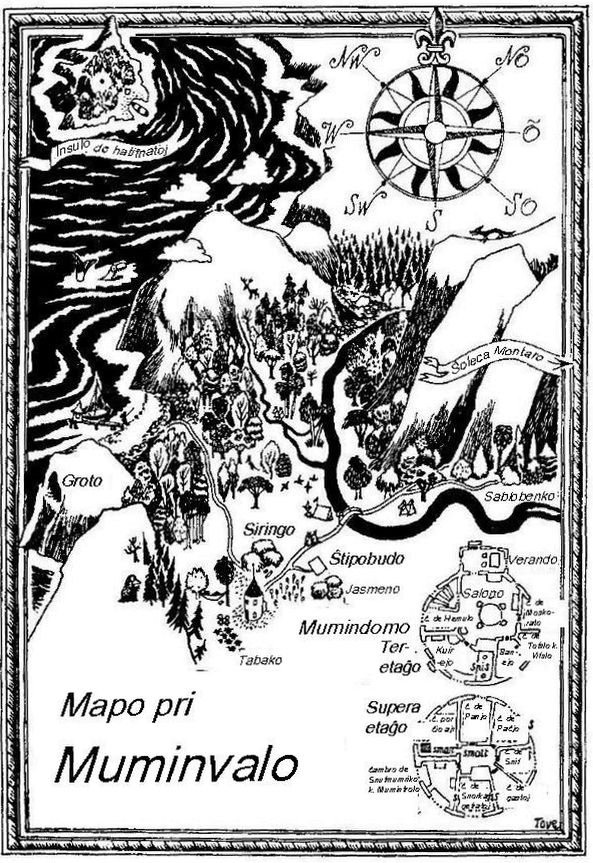
\includegraphics[width=394pt,height=580pt]{map-bildo.png}
\caption{}
\label{map-bildo}
\end{figure}

\chapter*[Ĉapitro 1]{Ĉapitro 1}
\addcontentsline{toc}{chapter}{Ĉapitro 1}


\begin{figure}[htbp]
\centering
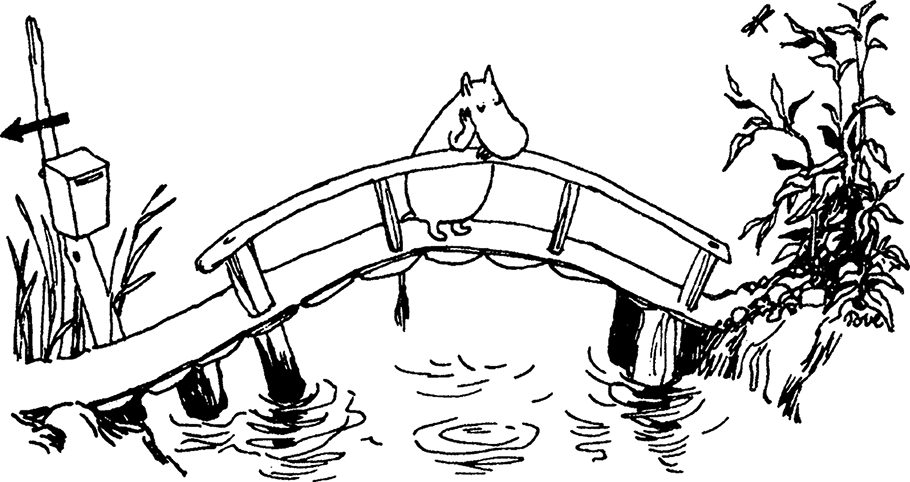
\includegraphics[width=450pt,height=237pt]{1-1.png}
\caption{}
\label{1-1}
\end{figure}

En la sama mateno, kiam la patro de Mumintrolo pretigis ponton trans la riveron, la besteto Snif faris eltrovon. Li trovis tute novan vojon. Ĝi enŝteliĝis en la arbaron en malluma loko, kaj Snif longe rigardis al ĝi.

`Ĉi tion mi rakontos al Mumintrolo,' li pensis. `Ni devos kune esplori tiun vojon, ĉar mi ne riskos tion sola.'

Poste li metis du branĉetojn kruce por retrovi la lokon kaj salte kuris hejmen plejeble rapide.

La valo kie ili loĝis estis tre bela. Ĝi estis plena de feliĉaj bestetoj kaj verdaj arbegoj. Tra la herbejoj fluis la rivero, ĝi faris kurbon ĉirkaŭ la blua mumindomo kaj malaperis al aliaj lokoj kun aliaj bestetoj, kiuj demandis sin de kie ĝi venas.

`Estas io stranga pri vojoj kaj riveroj,' Snif pensis, `oni vidas ilin preterpasi kaj ekhavas teruran emon esti aliloke. Akompani por vidi kie ili finiĝas{\ldots}'
\sectionbreak
Mumintrolo estis okupita fiksi pendolilon, kiam Snif revenis hejmen.

``Saluton,'' Snif diris. ``Mi trovis tute propran vojon. Ĝi aspektas danĝera.''

``Kiom danĝera?'' Mumintrolo demandis.

``Mi prefere dirus \emph{enorme} danĝera,'' la besteto Snif serioze respondis.

``Do ni devas kunporti buterpanojn,'' Mumintrolo diris.

\begin{figure}[htbp]
\centering
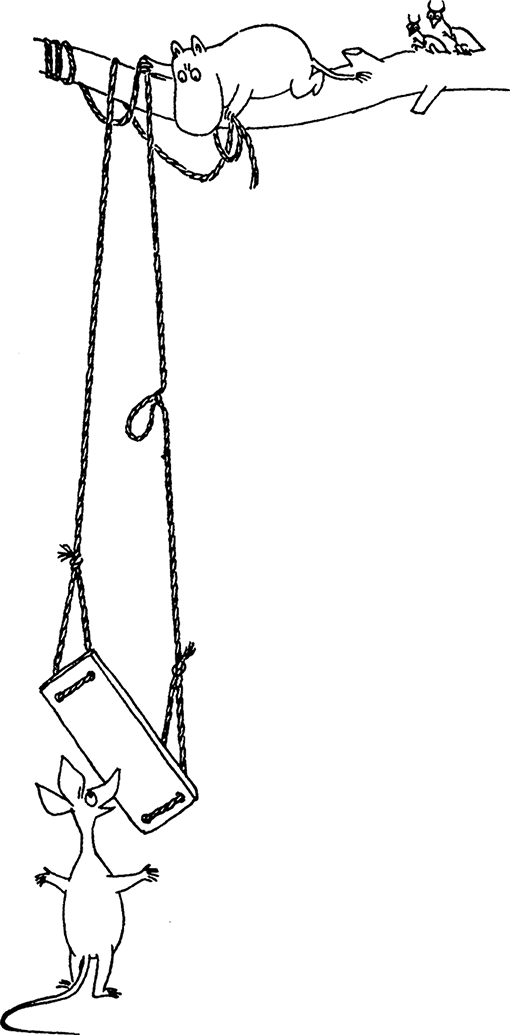
\includegraphics[width=150pt,height=305pt]{1-2.png}
\caption{}
\label{1-2}
\end{figure}

``Kaj fruktsukon.'' Li iris ĝis la kuireja fenestro kaj diris: ``Hej, Panjo. Hodiaŭ ni manĝos eksterdome.''

``Bone,'' la patrino diris. ``Tion vi ja povas fari.'' Ŝi metis buterpanojn en la korbon, kiu staris apud la lavtablo. Poste ŝi prenis muminmanplenon da bombonoj el unu skatolo kaj du pomojn el alia, kvar kolbasetojn de hieraŭ kaj botelon da preta fruktsuko, kiu kutime staris sur la forna breto.

``Tre bone,'' Mumintrolo diris. ``Ĝis baldaŭ. Ni do revenos kiam ni venos.''

``Ĝis la,'' respondis la patrino.

Mumintrolo kaj Snif iris tra la ĝardeno, trans la herbejojn kaj supren laŭ la deklivo, ĝis la malluma arbaro en kiun ili neniam eniris. Tie ili metis la korbon surteren kaj rigardis malsupren al la valo. La mumindomo estis malgranda kiel punkto, kaj la rivero aspektis kiel mallarĝa verda rubando. La pendolilo tute ne videblis de ĉi-supre.

``Vi neniam antaŭe estis tiel malproksime de via panjo,'' diris la besteto Snif. ``Nur mi estis ĉi tie, tute sola. Kaj nun vi vidos mian novan vojon kiun mi mem trovis.''

Li kuradis tien-reen, flaris kaj nazumis kaj rigardis la sunan altecon kaj ĉiel kondutis kaj finfine li kriis: ``Jen! Mi trovis ĝin! Nu? Kion vi diras? Ĉu ĝi ne aspektas danĝera? Vi iru la unua.''

Mumintrolo eniris la verdan mallumon, tre singarde. Ĉirkaŭ ili iĝis tute silente.

``Vi devas atenti danĝerojn el ĉiuj flankoj,'' Snif flustris.

``Mi ne povas samtempe rigardi ĉien,'' Mumintrolo kontraŭis. ``Vi rigardu malantaŭen, ĉar por tio mi ne havas tempon.''

``Ne, ne, malantaŭen ne,'' Snif timeme diris. ``Estas multe pli terure se iu postsekvas, ol se oni renkontas iun! Ĉi tio estos je via risko!''

\begin{figure}[htbp]
\centering
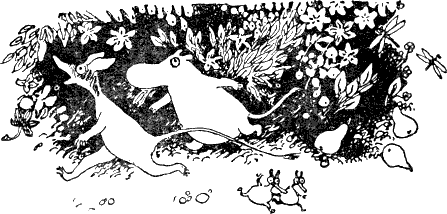
\includegraphics[width=450pt,height=214pt]{1-3.png}
\caption{}
\label{1-3}
\end{figure}

``Nu, do iru antaŭe,'' diris Mumintrolo.

``Ankaŭ tion mi ne volas!'' kriis Snif. ``Ĉu ni ne povas iri unu apud la alia?''

Do ili iris unu proksime apud la alia pluen kaj pluen en la arbaron. Ĝi iĝis pli kaj pli verda kaj malluma, kaj unue la vojo iris supren kaj poste malsupren kaj ĝi pli kaj pli mallarĝiĝis kaj fine restis entute neniu vojo, nur muskoj kaj filikoj.

``Vojo devas konduki ien,'' diris Mumintrolo. ``Ĉi tio estas malĝusta. Ĝi ne rajtas tiel finiĝi, tutsimple.'' Li faris kelkajn paŝojn sur la muskoj.

``Sed eble ni neniam retrovos la vojon hejmen,'' flustris Snif.

``Silentu iomete,'' diris Mumintrolo. ``Ĉu vi aŭdas ion?''

Fore trans la arboj aŭdiĝis mallaŭta susuro. Denove li faris kelkajn paŝojn, levis la nazon flarante. La vento estis humida kaj agrable odoris.

``Jen la maro,'' Mumintrolo kriis kaj ekkuris, ĉar se li amis ion entute, tio estis bani sin.

``Atendu!'' kriis Snif. ``Ne lasu min sola!''

Sed Mumintrolo haltis nur vidante la maron antaŭ si. Tiam li solene sidiĝis sur la sablon kaj rigardis la ondojn kiuj ruliĝadis, unu post alia, ĉiuj kun rando el blanka ŝaŭmo sur la pinto. Post kelka tempo Snif elvenis el la arbaro kaj sidiĝis apud li dirante: ``Vi forkuris de mi. Vi lasis min en la danĝero!''

\begin{figure}[htbp]
\centering
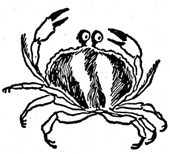
\includegraphics[width=100pt,height=90pt]{1-4.png}
\caption{}
\label{1-4}
\end{figure}

``Mi tiel ekĝojis,'' Mumintrolo klarigis. ``Mi konis la valon kaj la riveron kaj la montojn, sed ne ke ni krome havas maron. Rigardu kiaj ondoj!''

``Ili aspektas malvarmaj kaj koleraj,'' diris Snif. ``Ene de ili oni malsekiĝas, kaj sur ili oni vomemas.''

``Ĉu vi ne ŝatas plonĝi?'' Mumintrolo surprizite demandis. ``Ĉu vi povas plonĝi kun malfermitaj okuloj?''

``Mi povas, sed mi ne volas,'' diris Snif. Mumintrolo stariĝis kaj iris rekte kontraŭ la maron.

``Tio okazos je via risko!'' kriis Snif. ``Ne eblas antaŭe scii, kion oni ekvidos tie sube!''

Sed Mumintrolo plonĝis en grandan ondon tra kiu la suno klare brilis.

\begin{figure}[htbp]
\centering
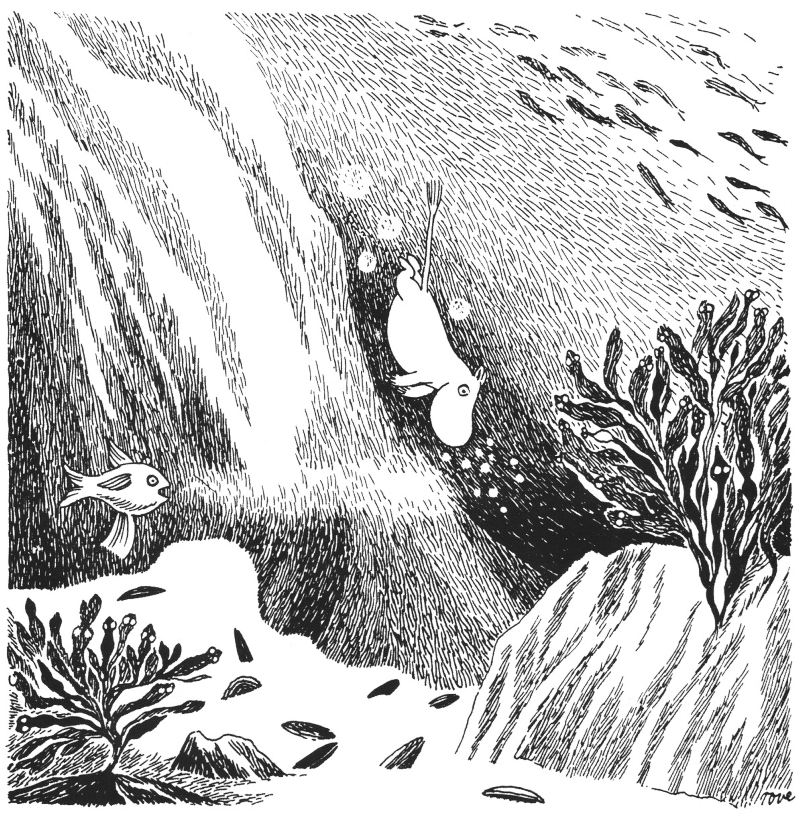
\includegraphics[width=450pt,height=459pt]{1-5.png}
\caption{}
\label{1-5}
\end{figure}

Unue li vidis nur verdajn vezikojn el lumo, poste li vidis arbarojn el fukoj kiuj balanciĝis super la sablo. Ili estis elegante frizitaj kaj ornamitaj per konkoj, interne rozkoloraj kaj ekstere blankaj. Pli fore de la tero la akvo malheliĝis proksime al nigra truo, kiu kondukis rekte suben en la senfundon. Tiam li returnis sin, sagis supren meze de ondo kaj akompanis ĝin reen al la strando. Tie Snif sidis vokante pri helpo.

``Mi pensis ke vi dronis!'' kriis Snif. ``Aŭ ke ŝarko formanĝis vin! Kio okazus al mi sen vi?''

``Ne stultumu,'' diris Mumintrolo. ``Mi kutimas je la akvo.''

Cetere, dum mi estis tie sube mi ekhavis ideon. Tre bonan ideon kiu estas sekreto.

``Kiom granda?'' demandis Snif. ``Ĉu same granda kiel ``abismo min glutu''?''

Mumintrolo kapjesis.

``Abismo min glutu,'' Snif recitis. ``Vulturoj manĝu miajn sekajn ostojn kaj neniam plu mi manĝu glaciaĵon se mi ne gardos la sekreton de l' sekretoj. Nu?''

``Mi estos perloĉasanto kaj kaŝos miajn perlojn en skatolo,'' diris Mumintrolo. ``Ĉiuj blankaj ŝtonoj estas perloj. Ĉiuj blankegaj kaj rondegaj.''

``Ankaŭ mi volas esti perloĉasanto!'' kriis Snif. ``Mi kaptos ilin surstrande. La tuta strando estas plena de ŝtonoj blankaj kaj rondaj.''

``Vi ne komprenas,'' Mumintrolo klarigis. ``Ili estas perloj nur sub la akvo. Ĝis baldaŭ.'' Kaj jen li refoje vadis eksteren tra la surfo.

``Kio do mi povas esti!?'' Snif kriis post li.

``Vi povas esti tia ulo, kiu trovas skatolon por perloĉasanto,'' diris Mumintrolo kaj plonĝis. Snif malrapide plupaŝis laŭ la strando.

``Vi prenas ĉion amuzan,'' li murmuris. ``Nur pro tio ke mi estas tre malgranda.''

Li iom serĉis skatolojn, sed troviĝis neniu. Nur fukoj kaj kelkaj tabulstumpoj. La strando estis longa kaj soleca kaj ĝi finiĝis per alta monto kiu deklivis rekte suben en la akvon. La tuta monto estis malseka de onda ŝaŭmo.

`Ĉi tio ne plu estas amuza,' pensis Snif. `Mi ne plu volas esti malgranda kaj sen iu kunludanto{\ldots}'

\begin{figure}[htbp]
\centering
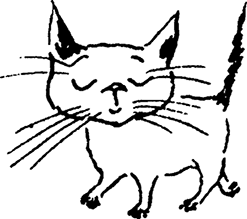
\includegraphics[width=100pt,height=88pt]{1-6.png}
\caption{}
\label{1-6}
\end{figure}

Kaj ĝuste tiam la besteto Snif ekvidis katidon kiu promenis sola plej supre sur la monto. Ĝi estis nigra-kaj blankmakula kaj havis tre mallarĝan voston kiu elstaris rekte supren. Li tiel ekĝojis ke tio doloris al li.

``Kateto,'' vokis Snif. ``Eta katideto,'' venu suben renkonti min, mi tiel terure enuas!

La katido sendis al li flavan rigardon trans la ŝultron kaj plu plandis.

Tiam Snif komencis grimpi. Li grimpis kaj grimpegis sur la malseka kruta monto, senĉese vokante al la kato. Kiam li finfine alvenis supren, ĝi jam plandis rekte antaŭen laŭ la krutaĵo kaj iris ekvilibre sur mallarĝa roka kornico.

``Ne foriru de mi!'' kriis Snif. ``Vi plaĉas al mi!''

Sed la katido plupaŝis, pli kaj pli foren. Sub la monto la maro muĝis.

La besteto Snif sentis siajn krurojn moliĝi. Lia koro ekbatis.

Kaj tiam li rampis post la katido. Li rampis tre malrapide senĉese pensante: mola ĉarma katideto kiu estas la mia{\ldots} kiu estas eĉ pli malgranda ol mi{\ldots} Ho, protektanto de ĉiuj bestetoj, mi petas, bonvolu lasi min havi ĝin kaj lasu min imponi al Mumintrolo{\ldots}

\begin{figure}[htbp]
\centering
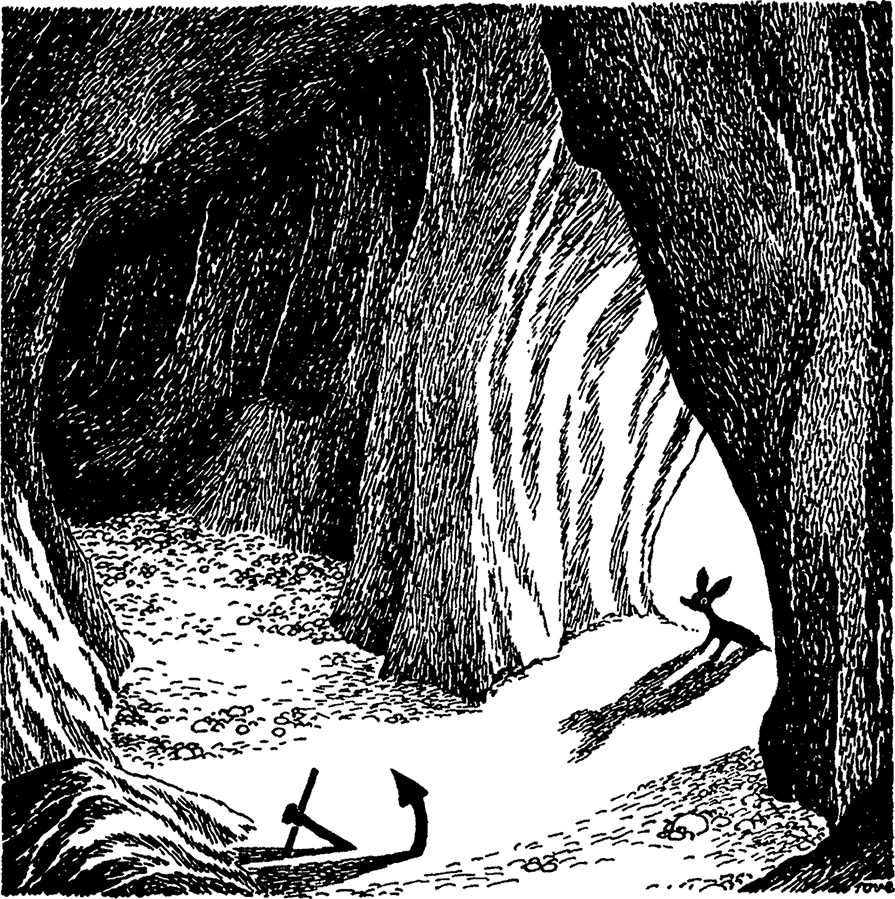
\includegraphics[width=450pt,height=452pt]{1-7.png}
\caption{}
\label{1-7}
\end{figure}

Neniam antaŭe li tiel timis kaj neniam sentis sin tiel kuraĝa. Kaj subite la groto troviĝis tie. Truo en la roka muro kaj trans ĝi vera groto.

Snif retenis la spiradon. Jen groto, kian oni trovas nur unufoje en la vivo, aŭ eble neniam. Ĝi havis subtilan sablan grundon kaj glatajn malhelajn murojn. Supre en la plafono troviĝis blua ĉiela fenestro. La sablo estis varma pro sunbrilo.

Li enrampis kaj kuŝiĝis surventre en la sunstrio pensante: jen mi loĝos dum mia tuta vivo. Mi metos etajn bretojn kaj faros dormejon sur la sablo kaj havos brulantan kandelon vespere. Kion diros Mumintrolo?

Sed la malamikema katido jam malaperis.
\sectionbreak
La vojo reen ne ŝajnis tre danĝera. Kiel io povus trafi tiun, kiu ĵus trovis groton?

Mumintrolo ankoraŭ okupiĝis pri sia perloĉasado. Li saltadis kiel korko sur la ondoj kaj surstrande kuŝis amaso da rondaj blankaj ŝtonoj.

``Nu, jen vi estas,'' li diris. ``Kie estas la skatolo?''

``Venu surteren! Tuj venu surteren!'' kriis Snif. ``Mi trovis ion!''

Mi trovis ion tute sola kaj kun la plej terura danĝero kiun vi povas imagi!

\begin{figure}[htbp]
\centering
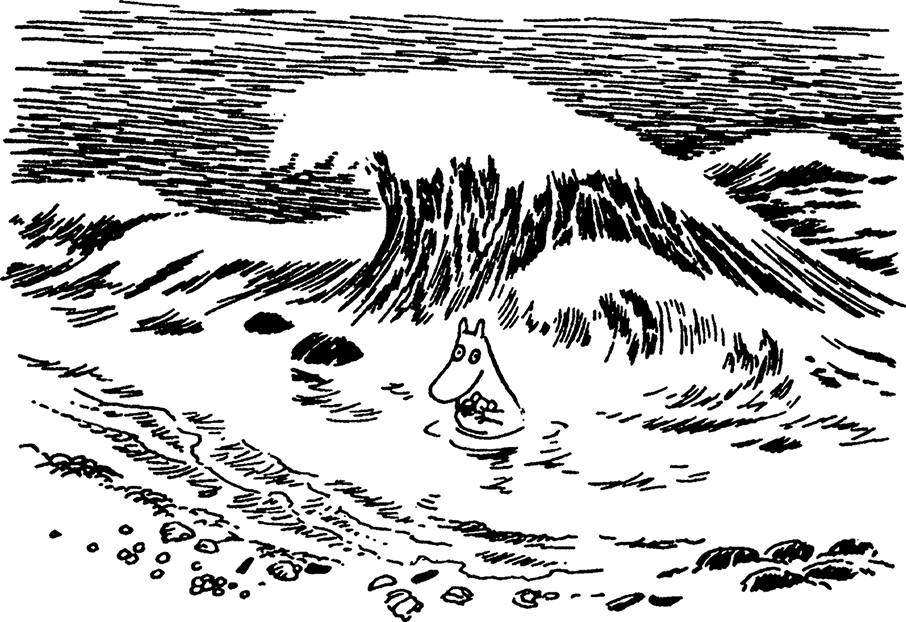
\includegraphics[width=450pt,height=307pt]{1-8.png}
\caption{}
\label{1-8}
\end{figure}

``Ĉu ĝi estas bona skatolo?'' demandis Mumintrolo kaj alvadis kontraŭ la strandon kun muminmanoj plenaj de perloj.

``Skatolo, skatolo,'' kriis Snif. ``konservu viajn skatolaĉojn! Abismo vin glutu kaj tiel plu, ni ne havas tempon por tio ĉar mi trovis groton! Propran groton!''

``Ĉu ĝi estas vera?'' demandis Mumintrolo. ``Kun grundo kaj truo por enrampi? Kun rokaj muroj kaj sabla grundo?''

``Ĉio! Ĉio necesa!'' respondis Snif kaj estis tiel ekster si, ke li apenaŭ restis staranta. ``Kaj vi rajtas konservi viajn perlojn en mia groto se vi donos al mi la duonon aŭ almenaŭ tri manplenojn!''
\sectionbreak
La perloj iĝis multe pli veraj kaj blankaj tuj veninte en la groton.

Mumintrolo kaj Snif kuŝis surdorse sur la sablo rigardante supren tra la blua ĉiela fenestro. Jen kaj jen salaj gutoj alflugis tra la pordo, kaj la sunstrio pli kaj pli larĝiĝis.

Snif tre deziris rakonti pri la katido. Sed li decidis ne fari tion.

Unue li trovos ĝin kaj amikiĝos kun ĝi. Ĝi akompanos lin ĉie. Kaj en unu hela tago ili kune venos en la verandon, kaj Mumintrolo diros: `Ĉu tio eblas!? Ĉu vi havas propran katidon kiu akompanas vin ĉie!?'

Oni povus meti subtason da lakto en la ĝardeno. Ĉiuvespere{\ldots}

Snif suspiris.

``Nun mi malsatas,'' li diris. ``Imagu, ke eblas iĝi tiel feliĉa ke oni forgesas manĝi!''
\sectionbreak
Nur malfrue posttagmeze Mumintrolo kaj Snif revenis al la blua domo en la valo. Dum la vespero proksimiĝis, la rivero fluis malrapide, kaj super ĝi la nova ponto brilis en multaj ĵuspentritaj koloroj. La patrino de Mumintrolo aranĝis konkojn ĉirkaŭ la florbedoj.

``Ĉu vi amuziĝis?'' ŝi demandis.

\begin{figure}[htbp]
\centering
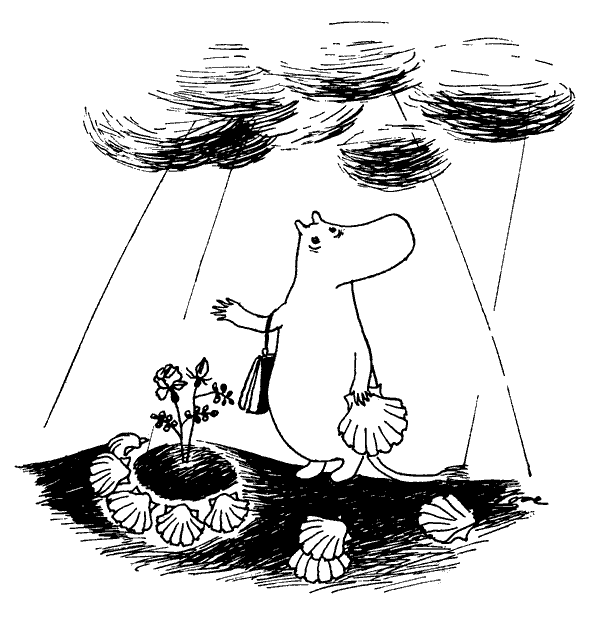
\includegraphics[width=359pt,height=371pt]{1-9.png}
\caption{}
\label{1-9}
\end{figure}

``Ni iris almenaŭ dek mejlojn for de ĉi tie!'' rakontis Mumintrolo. ``Mi vidis la maron! Mi plonĝis en grandegaj ondoj kaj trovis ion terure belan kiu komenciĝas per P kaj finiĝas per J{\ldots} Sed mi ne povas diri kio ĝi estas, ĉar ĝi estas sekreto!''

``Kaj mi trovis ion kio komenciĝas per G kaj finiĝas per O!'' kriis Snif. ``Kaj ie meze troviĝas O kaj T. Sed pli ol tion mi ne diros!''

``Kiel mirinde,'' diris Muminpanjo. ``Tiom da grandaj eventoj en unu tago. La supo staras en la varmujo. Kaj ne tro multe klaktintigu, ĉar via patro verkas.''

Poste ŝi pluis distribui konkojn, laŭvice unu bluan, du blankajn kaj unu ruĝan, kaj tio iĝis tre bela.

Ŝi malrapide fajfis al si mem pensante, ke aspektas kvazaŭ pluvos.

Malkvieta vento pasis tra la arboj, kiuj suspiris kaj skuis sin kaj turnis ĉiujn foliojn inverse. Longaj, grizaj nuboj ekvelis tra la ĉielo.

`Mi esperas ke ne denove estos inunda pluvo,' pensis la patrino de Mumintrolo. Ŝi kolektis kelkajn konkojn superfluajn kaj eniris en la domon ĝuste kiam ekfalis la unuaj gutoj.

Snif kaj Mumintrolo endormiĝis meze sur la salona tapiŝo. La patrino etendis plejdon sur ilin kaj sidiĝis ĉefenestre por rigardi la pluvon.

Ĝi estis griza pluvego kiu kunportis fruan krepuskon. Ĝi silente fingrumis sur la tegmento, lirlis en la ĝardeno, susuris tra la arbaro kaj malproksime ĝi gutadis en la groton de Snif.

Ie en sekreta kaj tute privata kaŝejo la malamikema katido volvis sian voston ĉirkaŭ si kaj endormiĝis.
\sectionbreak
Malfrue nokte, kiam ĉiuj jam enlitiĝis, la patro de Mumintrolo aŭdis plendan sonon. Li eksidis por aŭskulti. Pluvo torentis tra la defluaj tuboj kaj la difektita tegmenta fenestro kiel kutime batadis en la vento. Nun reaŭdiĝis la mizera sono. La patro surmetis negliĝon kaj iris prizorgi sian domon. Li esploris la bluan ĉambron, poste la flavan kaj fine la punktitan, kaj ĉie estis silente. Tiam la patro malfermis la verandan pordon kaj rigardis eksteren en la pluvon. Per sia poŝlampo li lumigis sur la ŝtuparo kaj herbejo, kaj la lumo glimigis la pluvgutojn kvazaŭ diamantojn. Nun blovis eĉ pli ol iam.

``Je kukolo, kio estas tio?'' diris la patro de Mumintrolo.

\begin{figure}[htbp]
\centering
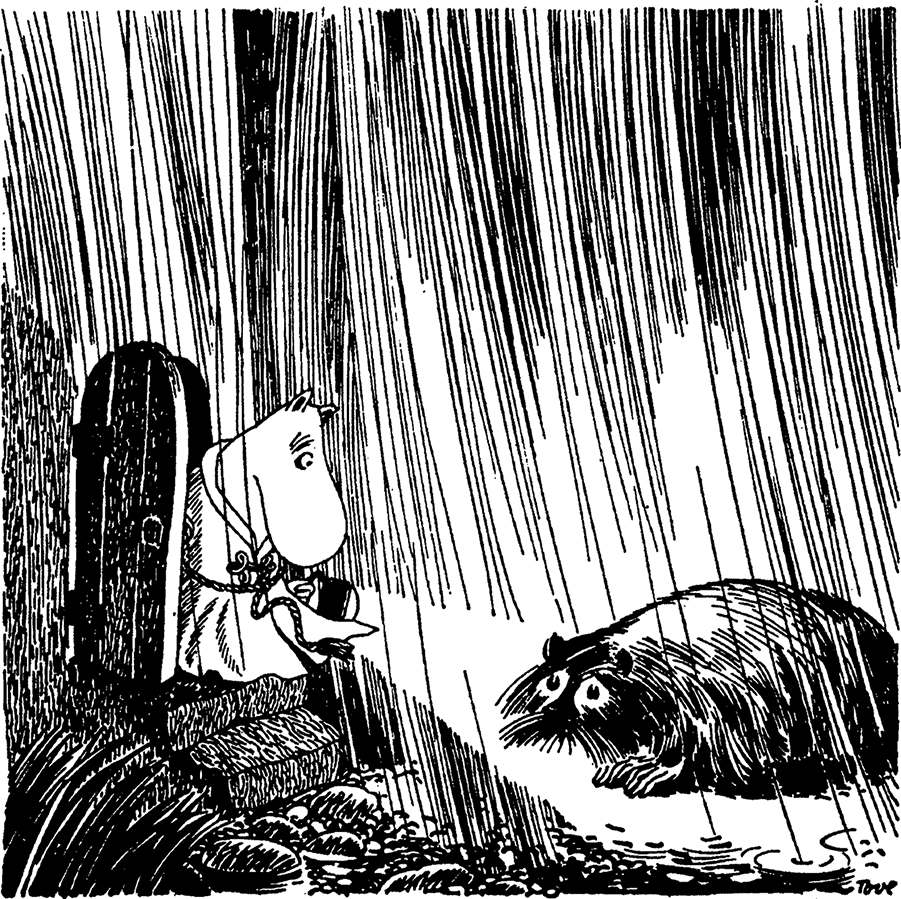
\includegraphics[width=450pt,height=450pt]{1-10.png}
\caption{}
\label{1-10}
\end{figure}

Ĉar ekstere sidis io malseka kaj mizera kun lipharoj kaj nigraj brilaj okuloj.

``Mi estas moskorato,'' diris la mizera estaĵo per malforta voĉo. ``Senhejma moskorato. Duono de la domo fendiĝis, kiam vi konstruis vian ponton trans la riveron. Tio kompreneble ne gravas. La dua duono malaperis pro la pluvo. Tio gravas eĉ malpli. Por filozofo estas tute egale, ĉu li vivas aŭ mortas, sed post tiu ĉi malvarmumo estas tre malcerte, kio okazos al mi{\ldots}''

``Mi terure bedaŭras,'' diris la patro de Mumintrolo. ``Mi ne sciis, ke vi loĝas sub la ponto. Envenu, pro ĉio! Sendube mia edzino povos aranĝi liton ie.''

``Mi ne tre zorgas pri litoj, ili estas tiel nenecesaj mebloj,'' la moskorato malĝoje diris. ``Mi loĝis en nura truo, sed mi bonfartis tie. Ja al filozofo egalas, ĉu li bonfartas aŭ ne, sed ĉiuokaze ĝi estis bona truo.''

Li deskuis de si akvon kaj aŭskultis ĉiudirekten. ``Kia domo estas tio ĉi?'' li demandis.

``Tute ordinara mumindomo,'' respondis la patro.``Mi mem konstruis ĝin. Kion vi dirus pri glaso da pomvino kontraŭ la malvarmumo?''

``Tio ja ne estas necesa,'' diris la moskorato. ``Sed eble tamen.''

La patro de Mumintrolo ŝteliris en la kuirejon kaj malfermis la ŝrankon sen lumigi. Li streĉis sin al la pomvina botelo, kiu staris sur la plej supra breto, streĉis kaj streĉadis sin, kaj subite li faligis bovlon kaj estiĝis terura krako. La tuta domo vekiĝis, oni vokis kaj batis per pordoj, kaj jen la patrino de Mumintrolo alkuris kun kandelo enmane.

``Ĉu estas nur vi,'' ŝi diris. ``Mi pensis ke iu fripono eniris al ni.''

``Mi volis subenigi la pomvinon,'' diris la patro. ``Kaj jen iu azeno metis tiun stultan bovlon tute ĉe la rando.''

``Estas tute bone ke ĝi dispeciĝis, ĝi estis malbelega,'' diris Muminpanjo. ``Estas pli facile se vi suriras seĝon. Kaj prenu glason ankaŭ por mi.''

\begin{figure}[htbp]
\centering
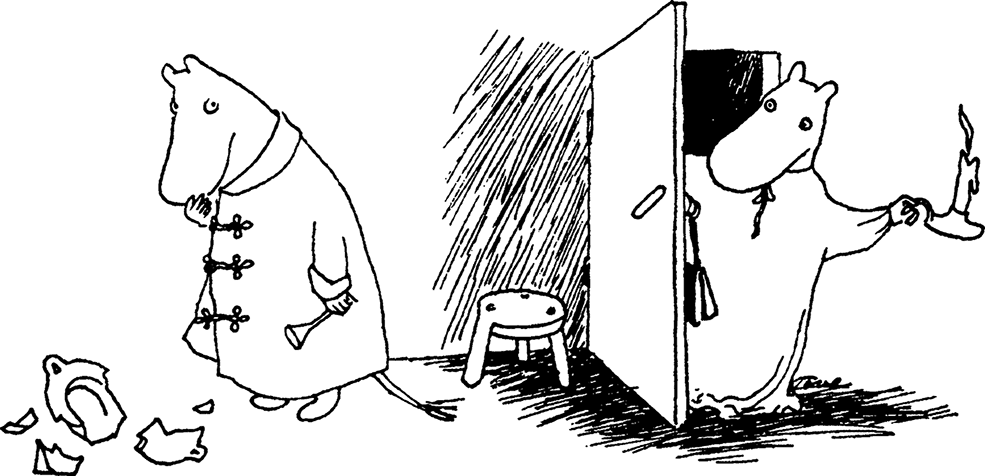
\includegraphics[width=414pt,height=200pt]{1-11.png}
\caption{}
\label{1-11}
\end{figure}

La patro suriris seĝon kaj kaptis la botelon kaj tri glasojn.

``Por kiu estas la tria?'' scivolis la patrino.

``Por la moskorato,'' respondis la patro. ``Lia domo difektiĝis, do li venas por loĝi ĉe ni.''

Ili lumigis la petrollampon en la verando kaj tostis. Ankaŭ Mumintrolo kaj Snif rajtis partopreni, kvankam estis meze de la nokto. Sed ili trinkis lakton. Ankoraŭ la pluvo dancadis sur la tegmento, kaj la blovado eĉ pli intensiĝis. Ĝi hurlis tra la kamentubo, kaj la klapoj de la kahelforno timeme skuiĝis.

La moskorato almetis la nazon al la veranda fenestro gapante eksteren en la mallumon.

``Tio ĉi ne estas natura pluvo,'' li diris.

``Ĉu ne ĉiuj pluvoj estas naturaj?'' demandis la patro de Mumintrolo. ``Ĉu ankoraŭ glason?''

``Eble glaseton,'' diris la moskorato. ``Dankon, dankon. Nun mi sentas min pli bone. La granda pereo ne tiom zorgigas min, sed iel oni preferus ne havi malvarman ventron pereante.''

\begin{figure}[htbp]
\centering
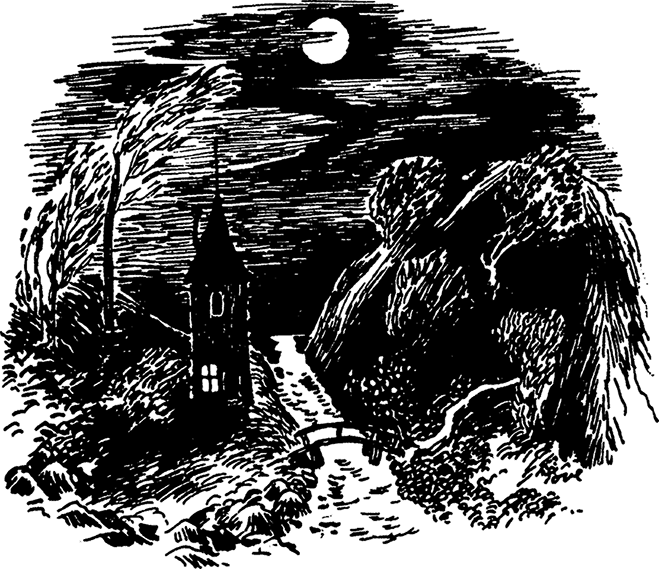
\includegraphics[width=322pt,height=278pt]{1-12.png}
\caption{}
\label{1-12}
\end{figure}

``Nu, certe ne,'' diris la patrino. ``Sed ĉi tio sendube ne estas inunda pluvo.''

La moskorato elsnufis.

``Vi ne scias pri kio mi parolas, sinjorino,'' li diris.``Ĉu vi lastatempe ne sentis ion strangan en la aero? Ĉu vi ne havis antaŭsentojn? Ĉu ne de temp' al tempo io tremigas vian nukon?''

``Nee,'' Muminpanjo surprizite diris.

``Ĉu io danĝera?'' flustris Snif gapante al la moskorato.

``Ne eblas scii,'' murmuris la moskorato. ``La universo estas tiel granda kaj la tero tiel terure malgranda kaj mizera{\ldots}''

``Nun mi opinias, ke ni enlitiĝu,'' la patrino rapide diris.

``Timigaj rakontoj malfrue nokte neniam estas bona afero.''

Post kelka tempo ĉiuj lumoj estingiĝis kaj la tuta domo dormis. Sed la pluvo kaj ŝtormo daŭris ĝis la sekva mateno.

\chapter*[Ĉapitro 2]{Ĉapitro 2}
\addcontentsline{toc}{chapter}{Ĉapitro 2}


\begin{figure}[htbp]
\centering
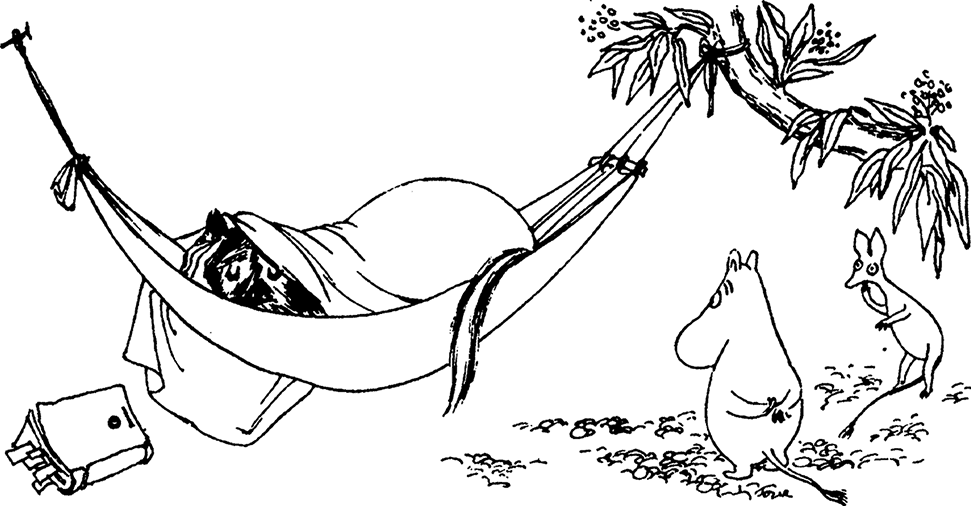
\includegraphics[width=450pt,height=234pt]{2-1.png}
\caption{}
\label{2-1}
\end{figure}

La sekva tago estis nuba. Mumintrolo vekiĝis kaj eliris en la malsekan silentan ĝardenon. La ŝtormo estis for, la pluvado ĉesis. Sed nenio estis kiel kutime. Li longe staris rigardante kaj flarante ĉiudirekten antaŭ ol kompreni, kio okazis.

Ĉio estis griza! Ne nur la ĉielo kaj la rivero, sed la arboj, la tero, la domo! Ĉio estis tute griza kaj aspektis terure, kvazaŭ ne plu vivante.

``Kiel terure,'' Mumintrolo malrapide diris. ``Kiel terure!''

La moskorato elvenis el la domo kaj plandis ĝis la hamako de Muminpatro.

Ankaŭ la hamako estis griza. Li kuŝiĝis sur ĝin kaj rigardis supren al la grizaj pomarboj.

``Hej!'' vokis Mumintrolo. ``Kio okazis? Kial ĉio estas griza?''

``Ne ĝenu min,'' diris la moskorato. ``Kuru ludi. Ludi dum vi povas ludi. Ni ĉiuokaze povas nenion fari pri la afero, do plej bone estas preni ĝin filozofe.''

``Kiu afero?!'' kriis la trolo.

``La pereo de l' mondo, kompreneble,'' la moskorato trankvile klarigis.

Mumintrolo turnis sin kaj kuris en la kuirejon, kie lia patrino okupiĝis kuiri matenan kafon.

``Panjo!'' li kriis. ``Ĉio estas griza kaj la moskorato diras ke la mondo pereos! Venu vidi!''

La patrino forigis la kafon de la fajro kaj kuniris en la ĝardenon.

``Kiel ĉio aspektas,'' ŝi diris. ``Kiel eblas, ke tiel terure polviĝis!'' Ŝi frotis permane laŭ folio, kaj la mano iĝis tute griza kaj iomete glua.

``Li \emph{diris} ke ĝi estas nenatura pluvo,'' vokis Mumintrolo. ``Li diris ke estas io stranga en la aero kaj ke io tremigas lian nukon kaj ke la tero estas tro malgranda{\ldots}''

``La moskorato sendube nur estis iom afliktita,'' la patrino klarigis. ``Oni iĝas tia, se la domo rompiĝis kaj la ventro malvarmas. Post la kafo mi provos senpolvigi la plej gravan ĉi-ekstere. Nun restu trankvila kaj ne malnecese timigu Snif'on.''

Ŝi endomiĝis kaj trovis la patron de Mumintrolo. ``Ĉu vi jam vidis, kiel ĉio aspektas?'' ŝi diris.

``Jes ja,'' la patro diris kun interesiĝo. ``Mi flaris ĝin, kaj ĝi odoras je fosforo! Tre ekscita fenomeno.''

``Sed ĝi timigas la idojn,'' kontraŭis la patrino. ``Kaj la moskorato eĉ pli timigas ilin. Ĉu vi ne povas konvinki lin paroli pri agrablaj aferoj aŭ entute nenion diri?''

``Mi provos,'' Muminpatro promesis. ``Sed mi timas, ke li loĝadis sola tiom longe, ke li diras ion ajn kio plaĉas al li.''

\begin{figure}[htbp]
\centering
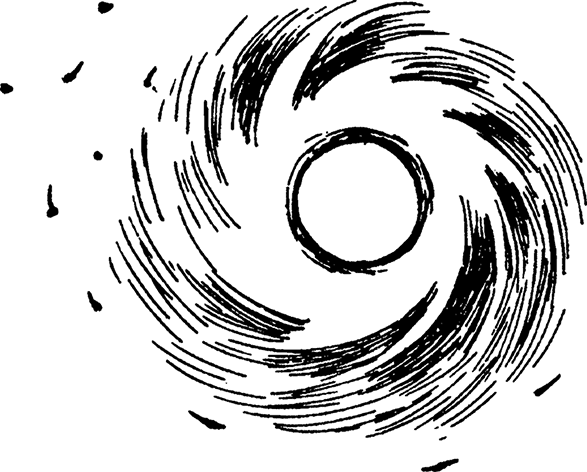
\includegraphics[width=234pt,height=190pt]{2-2.png}
\caption{}
\label{2-2}
\end{figure}

La patro pravis. Ĉe la matena kafo la moskorato konstruis la tutan universon sur la veranda tablo.

``Jen la suno,'' li diris montrante al la sukerujo. ``Ĉiuj ĉi biskvitoj estas steloj. Kaj ĉi tiu biskvit\emph{ero} estas la tero. Jen kiel malgranda ĝi estas! Kaj la universo estas tiel granda, ke ĝi neniam finiĝas. Ĝi estas tute karbe nigra. Kaj jen supre en la mallumo la monstroj de la ĉielo vagadas, la skorpio, la ursino kaj la kankro{\ldots}''

``Nu nu,'' la patro interrompis.

Sed la moskorato indiferente pluis: ``Kaj por la sekva sunsistemo eĉ ne estas loko sur via veranda tablo.Ĝi estas tie ekstere!'' Kaj jen la moskorato ĵetis buterpanon eksteren en la ĝardenon.

``Nu, bone,'' diris la patrino kaj formetis la restantajn buterpanojn. ``Ĉu troviĝas multaj sunsistemoj?''

``Amaso,'' respondis la moskorato kun malĝoja kontenteco. ``El tio ĉi vi povas kompreni, kiel malmulte tio signifas, ĉu la tero pereas aŭ ne.''

La patrino suspiris.

``Mi ne volas perei!'' kriis Snif. ``Mi trovis groton! Mi ne havas tempon perei!''

La patro klinis sin antaŭen al la moskorato kaj diris: ``Kion vi opinias pri iom da pensado sur la hamako? Ĉu tio ne estus agrabla?''

``Tiel vi diras nur por seniĝi de mi,'' diris la moskorato. Li blovis al la biskvitero kiu estis la tero, kaj ĝi malaperis trans la randon de la tablo. Mumintrolo ekĝemis.

``Nun ni tuj iru malsupren ĝis la rivero,'' diris Muminpanjo. ``Mi montros al vi kiel fari boatojn el kanoj.''
\sectionbreak
Tiu tuta tago estis tre malrapida. Snif kaj Mumintrolo ne emis iri ĝis la groto, ĉar imagu se la tero pereus dum ili estas for de hejme. Kapti perlojn subite ŝajnis tute stulte. Ili sidiĝis sur la ŝtuparon de la verando, kiu iel ŝajnis plej sekura, kaj flustre interparolis pri la universo, kiu tute ne estas blua sed nigra, kaj kie tuta sunsistemo ne signifas pli multe ol forĵetita buterpano.

``Ni devas igi ilin fari ion,'' la patrino zorgeme diris al la patro de Mumintrolo. ``Ili ne volas ludi. Ili povas pensi pri nenio krom tiuj pereaj ideoj, kiujn la moskorato glutigis al ili.''

``Mi pensas ke ni sendu ilin for de hejme dum kelka tempo,'' diris la patro. ``La moskorato parolas pri Observatorio.''

``Pri \emph{kio}?'' demandis Muminpanjo.

``Ob-ser-va-to-rio,'' diris la patro. ``Ĝi ŝajne situas ie malsupre laŭ la rivero. Iu loko kie oni observas stelojn. Se la idoj nun zorgas pri nenio krom steloj, do kial ili ne povu rigardi ilin?''

``Nu, pri tio vi eble tute pravas,'' respondis la patrino kaj pluis senpolvigi la siringan arbedon.

Kiam ŝi finpensis, ŝi paŝis ĝis la veranda ŝtuparo.

``Paĉjo kaj mi elpensis, ke vi faru etan ekskurson,'' ŝi diris.

``Kara panjo, oni ne ekskursas kiam la tero povas perei je ĉiu ajn momento,'' respondis Mumintrolo.

``La universo estas karbe nigra kaj plena de grandaj danĝeraj steloj,'' murmuris la besteto Snif.

``Mi scias,'' diris la panjo. ``Kaj ĝuste tiujn stelojn vi iru rigardi. La moskorato diris, ke troviĝas loko kie oni rigardas stelojn ne malproksime de ĉi tie. Povus esti utile por ni ĉi-hejme ekscii, \emph{kiom} grandaj tiuj steloj estas, kaj ĉu la universo efektive estas nigra.''

``Ĉu vi pensas, ke tio trankviligus vin?'' demandis Mumintrolo.

``Absolute,'' respondis lia panjo.

Mumintrolo tuj stariĝis kaj diris: ``Ni ekscios tion. Vi ne estu maltrankvila. Eble la tero estas multe pli granda ol oni kredas.''

La kruroj de Snif moliĝis pro ekscito, kaj li pensis: `Mi rajtas kuniri. Mi ne estas tro malgranda por kuniri!'

Li turnis sin al la patrino de Mumintrolo kaj diris: Ni zorgos pri la afero. Estu trankvila. Sed ne forgesu elmeti subtason da lakto sur la ŝtuparon ĉiutage dum mi estos for. Mi ne diras kial ĉar tio estas sekreto.''

\begin{figure}[htbp]
\centering
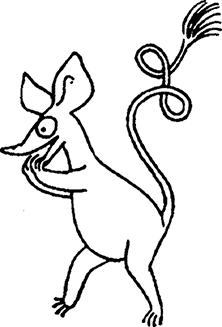
\includegraphics[width=100pt,height=147pt]{2-3.png}
\caption{}
\label{2-3}
\end{figure}

\chapter*[Ĉapitro 3]{Ĉapitro 3}
\addcontentsline{toc}{chapter}{Ĉapitro 3}


\begin{figure}[htbp]
\centering
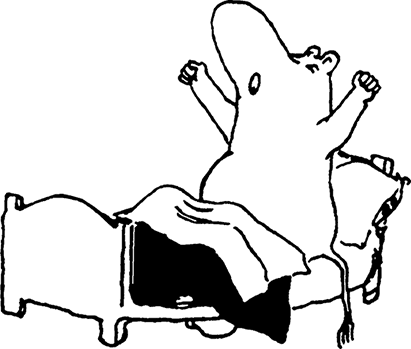
\includegraphics[width=189pt,height=160pt]{3-1.png}
\caption{}
\label{3-1}
\end{figure}

En la granda tago de vojaĝo Mumintrolo vekiĝis tre frue kaj kuris ĝis la fenestro por rigardi la veteron. Ankoraŭ restis nube. La nuboj pendis malalte super la deklivoj, kaj neniu folio moviĝis en la ĝardeno.

``Snif! Vekiĝu! Ni ekiros!'' vokis la trolo. Li kuris suben laŭ la ŝtuparoj, li sentis sin kuraĝega kaj tre forta. La patrino okupiĝis pri pakado. Ŝi faris buterpanajn pakojn, kaj sur la salona tablo staris amaso da dorsosakoj, korboj kaj skatoloj.

``Kara panjo,'' diris Mumintrolo. ``Ni absolute ne povas kunporti ĉion tie. Oni ridos pri ni.''

``Estas malvarme en Soleca Montaro,'' diris la patrino kaj enŝovis du trikitajn jakojn kaj unu krespetopaton. ``Ĉu vi havas la kompason?''

``Jes ja,'' respondis Mumintrolo. ``Sed ĉu vi ne povas almenaŭ forigi la telerojn. Ni intencas manĝi sur verdaj folioj.''

\begin{figure}[htbp]
\centering
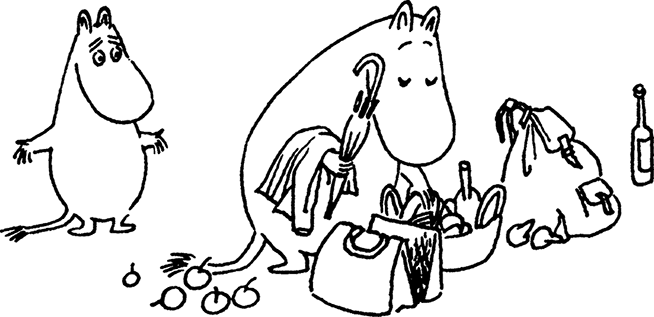
\includegraphics[width=331pt,height=160pt]{3-2.png}
\caption{}
\label{3-2}
\end{figure}

``Kiel plaĉas al vi, karulo,'' diris lia panjo kaj retiris la telerojn. ``Paĉjo pretigas la floson. La moskorato dormas. Kie estas Snif?''

``Jen,'' respondis Snif matene mishumore. Li estis tiel dormema ke lia tuta vizaĝo estis ĉifita. Li plandis eksteren sur la ŝtuparon, rigardis la laktan subtason kaj tuj vekiĝis. La subtaso ne plu estis plena, li estis certa ke la lakto malaltiĝis. La katido venis tien. Ĝi revenos, ĝi eble sidos atendante lin kiam li revenos hejmen. Poste la tuta universo povos enlitiĝi.

Ĉe la riverbordo la floso kuŝis preta kun levita velo.

``Memoru resti meze de la rivero,'' diris la patro. ``Kaj se vi vidos ion strangan kun ronda tegmento, ĝi estas observatorio. La moskorato diris, ke tie loĝas amaso da profesoroj kiuj zorgas pri nenio krom steloj. Grandaj kaj malgrandaj kaj tiom kiom vi deziros. Prenu la albordiĝan ŝnuron. Ĝis baldaŭ!''

``Ĝis la,'' vokis Mumintrolo kaj Snif. La floso ekflosis malsupren laŭ la rivero.

``Bonan ekskurson!'' vokis la patrino de Mumintrolo. ``Kaj revenu dimanĉe, ĉar tiam ni manĝos anĝelkaĉon. Ne forgesu surmeti la lanajn kalsonojn se estos malvarme! La stomakpulvoroj kuŝas en la maldekstra flanka fako{\ldots}''

Sed la floso jam preterflosis la unuan kurbiĝon, kaj antaŭ ili etendiĝis la rivero, neloĝata kaj alloga, foren al ĉio nekonata.
\sectionbreak
Iom post iom la bordoj iĝis pli altaj, malproksime altiĝis Soleca Montaro kiel ombro kontraŭ la ĉielo. La rivero estis same griza kiel la ĉielo, kaj estis tute silente. Neniu birdo kantis kaj neniu fiŝo kaptis ĉe la akvosurfaco. Kaj neniu sola observatorio.

La besteto Snif postulis stiri sed post kelka tempo tediĝis.

``Ĉu ni ne baldaŭ alvenos?'' li demandis.

``Ĉi tio estas tre granda kaj grava vojaĝo,'' respondis Mumintrolo. ``Ne multaj bestetoj havas okazon partopreni en tia.''

``Sed nenio okazas,'' kontraŭis Snif. ``Nur grizaj samaj bordoj kaj nenio por fari. Oni povus kapti perlojn kaj fari etajn bretojn en la groto{\ldots}''

``Perlojn,'' diris Mumintrolo. ``Tio ja estis nur blankaj ŝtonoj. Ĉi tio estas io serioza, komprenu. La tero povas perei ĉiumomente, kaj ni ekiris por ekscii, kion eblas fari pri la afero. Hieraŭ vi povis paroli pri nenio krom danĝeraj steloj.''

\begin{figure}[htbp]
\centering
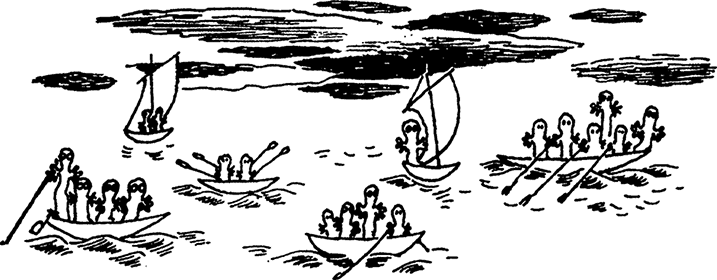
\includegraphics[width=321pt,height=125pt]{3-3.png}
\caption{}
\label{3-3}
\end{figure}

``Tio estis hieraŭ,'' diris Snif.

La rivero plufluis, griza kaj silenta. Je la krepusko ili vidis kvindekon da hatifnatoj vagantaj orienten.

``Ili ekiris malfrue ĉi-jare,'' diris Mumintrolo. ``Ĉu vi iam vidis ilin de proksime? Ili nenion diras kaj zorgas pri neniu. Nur iras kaj iras kaj gestas per la manoj kaj gapas al la horizonto. Paĉjo diras, ke ili neniam atingas tien, kien ili iras, kaj ĉiam sopiras aliloken{\ldots}''

Snif rigardis la hatifnatojn. Ili estis tre malgrandaj kaj blankaj kaj ne havis vizaĝojn.

``Ne,'' li diris. ``Mi vidis neniun de proksime, kaj mi ankaŭ ne volas tion. Ĉu ni ne baldaŭ alvenos?''

Mumintrolo suspiris kaj stiris la floson ĉirkaŭ la sekva kurbiĝo. Kaj jen li ekvidis ion strangan sur la rivera bordo, ion similan al klare flava sukerkonuso. Tio estis la unua gaja koloro kiun li vidis en la tuta tago.

``Kio estas tio?'' vokis Snif. ``Ĉu Observatorio?''

``Ne,'' diris Mumintrolo. ``Tio estas tendo. Flava tendo. Kaj en ĝi brilas lumo{\ldots}''

Kiam ili alproksimiĝis ili aŭdis iun ludi per buŝharmoniko en la tendo. Mumintrolo turnis la rudron kaj la floso malrapide turniĝis al la tero kaj stabile haltis ĉe la bordo.

``Hola?'' li mallaŭte vokis.

La muziko silentiĝis. Kaj el la tendo venis mumriko kun malnova verda ĉapelo kaj pipo enbuŝe.

\begin{figure}[htbp]
\centering
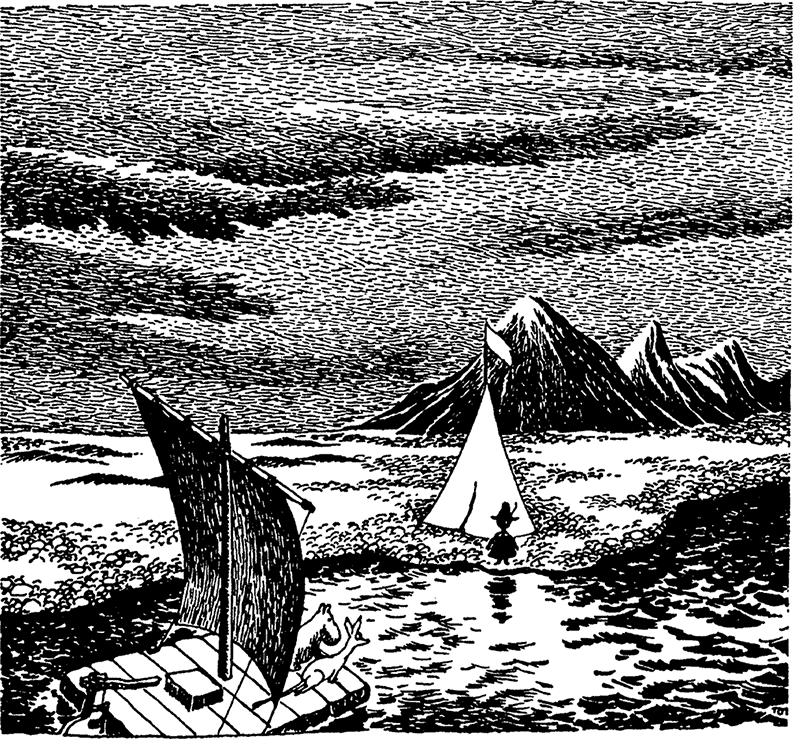
\includegraphics[width=450pt,height=419pt]{3-4.png}
\caption{}
\label{3-4}
\end{figure}

``Saluton,'' diris la mumriko. ``Ĵetu la ŝnuron al mi. Vi ne hazarde kunportas iom da kafo surŝipe?''

``Tutan skatolon!'' vokis Snif. ``Ankaŭ sukeron. Mi estas Snif kaj mi vojaĝis almenaŭ cent mejlojn kaj mi rajtis stiri preskaŭ la tutan vojon kaj hejme mi havas sekreton kiu komenciĝas per K kaj finiĝas per O! Jen Mumintrolo. Lia paĉjo konstruis tutan domon!''

``Ĉu vere?'' la mumriko diris rigardante ilin. ``Mi estas Snufmumriko.''

Li faris etan fajron ekster la tendo kaj ekkuiris kafon.

``Ĉu vi loĝas ĉi tie tute sola?'' demandis Mumintrolo.

``Mi loĝas jen kaj jen,'' respondis Snufmumriko eligante tri tasojn. ``Hodiaŭ hazarde estas ĉi tie, morgaŭ aliloke. Jen la avantaĝo loĝi en tendo. Ĉu vi survojas ien?''

``Jes. Al Observatorio,'' Mumintrolo serioze diris. ``Ni rigardos danĝerajn stelojn kaj ekscios, ĉu la universo efektive estas nigra.''

``Tio estos longa vojaĝo,'' diris Snufmumriko. Poste li silentis sufiĉe longe.

Kiam la kafo estis preta li verŝis ĝin en la tasojn dirante: ``Ne eblas scii pri kometoj. Ili venas kaj foriras laŭplaĉe. Eble ĝi tute ne venos ĉi tien.''

``Kio estas kometo?'' demandis Snif, kaj liaj okuloj nigriĝis.

``Ĉu vi ne scias tion?'' diris Snufmumriko. ``Tamen vi ekiris por rigardi danĝerajn stelojn? Kometo estas sola stelo kiu perdis la prudenton kaj ĵetas sin tra la universo kun arda vosto post si. Ĉiuj aliaj steloj havas bonordajn orbitojn laŭ kiuj ili iras, sed la kometo povas aperi ĉie ajn. Ankaŭ ĉi tie.''

``Kaj kio do okazos?'' flustris Snif.

``Malbono,'' diris Snufmumriko. ``La tuta tero dispeciĝos.''

``Kiel vi scias ĉion ĉi?'' bruske demandis Mumintrolo.

Snufmumriko levis la ŝultrojn.

``Homoj babilas,'' li diris. ``Ĉu vi volas pli da kafo?''

``Ne, dankon,'' diris la trolo. ``Mi ne emas je pli da kafo.''

``Ankaŭ mi ne!'' ekkriis Snif. ``Mi malbonfartas{\ldots} Baldaŭ mi vomos!''

Ili longe sidis rigardante al la dezerta pejzaĝo nenion dirante. Snufmumriko elpoŝigis la buŝharmonikon kaj ludis nedifinitan vesperan kanton.

Nun la danĝero ekhavis nomon. La kometo. Mumintrolo rigardis la ĉielon, kiu estis griza kaj ĉiutaga. Sed nun li sciis, ke ie trans la nuba kovrilo flugas la brulanta stelo, la kometo kun longa brilanta vosto, ĝi flugas pli kaj pli proksimen{\ldots}

``Kiam ĝi alvenos?'' li subite demandis.

``Tion oni sendube scias en tiu observatorio,'' diris Snufmumriko ekstarante. ``Sed certe ĝi ne venos ĉivespere. Ĉu ni faru etan promenon antaŭ ol mallumiĝos?''

``Kien?'' timeme demandis Snif.

``Ho, ien ajn,'' diris Snufmumriko. ``Sed se vi nepre deziras iri ien, ni ja povus rigardi la grenatan fendegon.''

\begin{figure}[htbp]
\centering
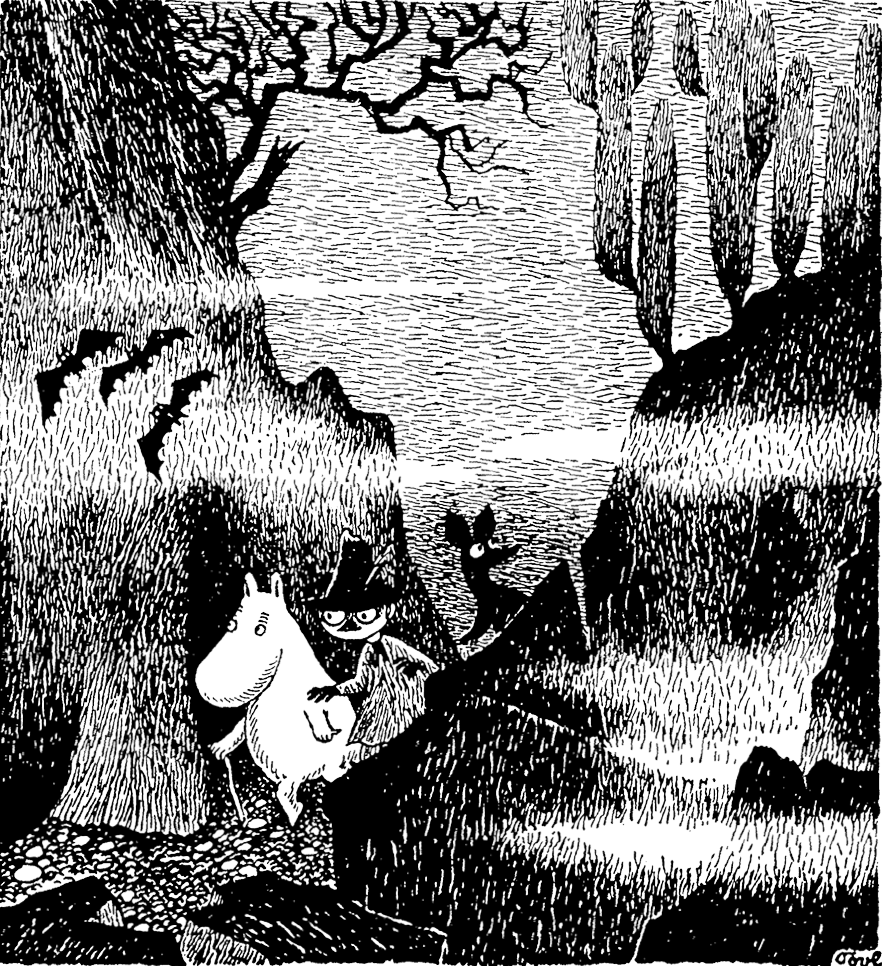
\includegraphics[width=425pt,height=463pt]{3-5.png}
\caption{}
\label{3-5}
\end{figure}

``Grenatoj!'' vokis Snif. ``Ĉu ili estas veraj?''

``Mi ne scias,'' respondis Snufmumriko. ``Sed ili estas belaj.''

Ili ekiris en la dezerton, paŝis singarde inter rokoj kaj dornaj arbedoj.

``Devus esti sunbrilo, tiam ili glimas eĉ pli,'' diris Snufmumriko.

Snif ne respondis. Liaj lipharoj staris supren pro atendoj, kaj li tute ne plu malbonfartis.

Nun ili palpiris antaŭen tra sovaĝa ravino, kie la teron trairis profundaj fendoj. Tie estis timige silente kaj forlasite en la krepusko, kaj ili interparolis flustre.

``Paŝu singarde,'' malrapide diris Snufmumriko. ``Jen estas.''

Ili klinis sin antaŭen kaj rigardis. Sube en la malvasta fendego glimis miriadoj da ruĝaj gemoj en la malaperanta lumo. Amaso da etaj kometoj en nigra universo{\ldots}

``Ĉu ili ĉiuj estas la viaj?'' flustris Snif.

``Dum mi loĝas ĉi tie,'' senzorge diris Snufmumriko. ``Mi posedas ĉion kion mi vidas kaj ŝatas. La tutan mondon, se vi volas.''

``Ĉu vi pensas, ke mi povus aĉeti kelkajn?'' sopire demandis Snif. ``Eblus aĉeti galeason per ili --- aŭ skutilon{\ldots}''

``Prenu kiom vi volas,'' ridante respondis Snufmumriko.

Snif komencis singarde grimpi suben en la fendegon. Li frotis al si la nazon kaj plurfoje preskaŭ falis, sed pluiris decide.

Kiam li finfine atingis la subon li profunde enspiris kaj komencis kolekti grenatojn per tremantaj manoj. Kio estis la perloj de Mumintrolo kompare kun ĉi tio? La glimanta amaso pli kaj pli grandiĝis, li iris pli kaj pli foren en la fendegon kolektante, tute silenta pro feliĉo.

``Hej,'' vokis Snufmumriko de supre. ``Ĉu vi ne baldaŭ revenos supren?''

``Ankoraŭ ne!'' kriis Snif. ``Restas tiom{\ldots}''

``La roso falas kaj estos malvarme,'' vokis Snufmumriko.

``Jes jes,'' diris Snif. ``Mi venos{\ldots} tuj{\ldots}'' Kaj li iris ankoraŭ pli profunden en la fendegon kie du grandaj ruĝaj grenatoj brilis kontraŭ li.

\begin{figure}[htbp]
\centering
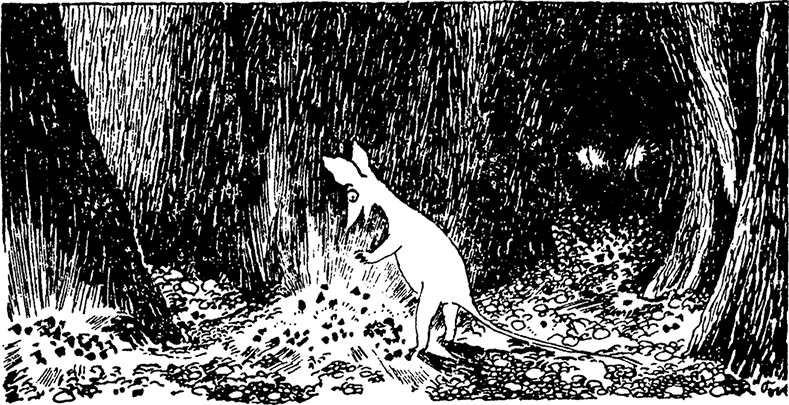
\includegraphics[width=440pt,height=225pt]{3-6.png}
\caption{}
\label{3-6}
\end{figure}

Tiam okazis la teruraĵo. La grenatoj moviĝis, ili palpebrumis. Ili alproksimiĝis. Kaj post ili sekvis skvama korpo kiu malvarme raslis kontraŭ la ŝtonoj. Snif kriis unu solan fojon, poste li turnis sin kaj kuris. Li saltis, ĵetiĝis, kuris, galopis antaŭen ĝis la roka muro kaj ekgrimpis per manoj kaj piedoj malsekaj pro teruro. Sub li io siblis malrapide kaj minace.

``Kio okazas al vi?'' demandis Mumintrolo. ``Kial vi tiel hastas?''

Snif ne respondis, li nur grimpis, kaj veninte super la randon li kolapsis kiel mizera amaseto.

\begin{figure}[htbp]
\centering
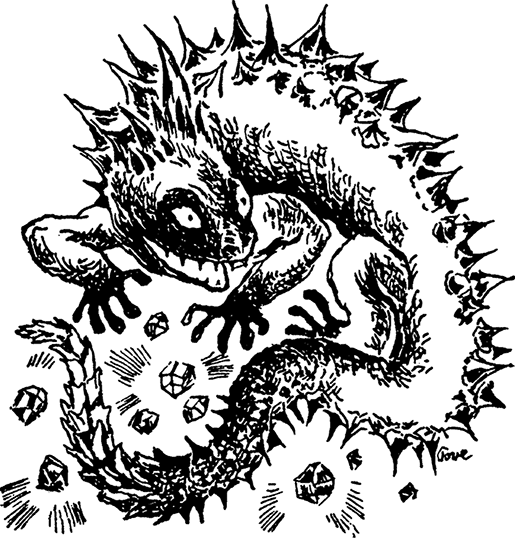
\includegraphics[width=249pt,height=261pt]{3-7.png}
\caption{}
\label{3-7}
\end{figure}

Mumintrolo kaj Snufmumriko klinis sin super la fendego kaj rigardis. Kaj tiam ili vidis la gigantan saŭron, kiu kaŭris super la amaso da grenatoj.

``Je mia vosto,'' flustris Mumintrolo.

Snif plorante sidis surtere.

``Tio jam pasis,'' diris Snufmumriko. ``Ne ploru, amiketo.''

``La grenatoj,'' singultis Snif. ``Eĉ ne unu solan mi ricevis!''

Snufmumriko sidiĝis apud lin kaj diris amike: ``Mi scias. Ĉio iĝas malfacila, kiam oni volas posedi aĵojn, kunporti ilin kaj havi ilin. Mi nur rigardas ilin, kaj kiam mi foriras, ili restas en mia kapo kaj mi povas fari ion pli amuzan ol porti valizojn.''

``Mi povus havi ilin en la dorsosako,'' Snif malgaje diris. ``Tute ne estas same rigardi aĵojn kiel palpi ilin kaj scii, ke ili estas miaj propraj.''

Li ekstaris kaj laŭte blovis la nazon permane. Poste ili paŝis penseme kaj iomete malĝoje reen tra la mallumiĝanta ravino.
\sectionbreak

\begin{figure}[htbp]
\centering
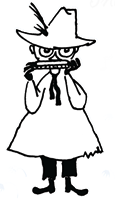
\includegraphics[width=86pt,height=150pt]{3-8.png}
\caption{}
\label{3-8}
\end{figure}

Snufmumriko faris la vojaĝon multe pli gaja. Li ludis kantojn, kiujn ili neniam antaŭe aŭdis, li instruis al ili ludi pokeron kaj fiŝkapti. Kaj li rakontis sovaĝajn kaj nekredeblajn historiojn.

Ankaŭ la rivero pli gajiĝis, ĝi fluis pli rapide kun etaj akvokirloj jen kaj jen. Ĝi jam estis pli mallarĝa, kaj Soleca Montaro alproksimiĝis.

Ĝiaj pintoj altiĝis en la nubojn, kiuj daŭre kuŝis kiel peza kovrilo super la tero. Sed neniu observatorio videblis.

``Rakontu ion,'' diris Snif. ``Ne pri kometoj. Ion amuzan.''

Snufmumriko sidis stirante.

``Ĉu vi volas aŭdi pri la fajrosputa monto?'' li demandis.

Ili serioze kapjesis.

Snufmumriko ŝtopis sian pipon kaj ekbruligis ĝin. Poste li diris: ``Okazis ĉi tiel, iufoje mi venis al loko, kie la tero estis nur nigra lafo. Sub la lafo io muĝis tage-nokte. Estis la tero, kiu kuŝis dormante tie interne kaj jen kaj jen moviĝis endorme. La lafaj blokoj estis ĵetitaj pelmele kaj super ili ŝvebis varmega vaporo, kiu igis ĉion aspekti malreale kaj strange. Mi venis tien iam vespere kaj efektive estis sufiĉe laca, do mi deziris iom da teo. Estis facile kuiri ĝin, oni simple plenigis la kaserolon per bolanta akvo el varmega fonto.''

``Ĉu oni ne brulvundiĝis,'' demandis Mumintrolo.

\begin{figure}[htbp]
\centering
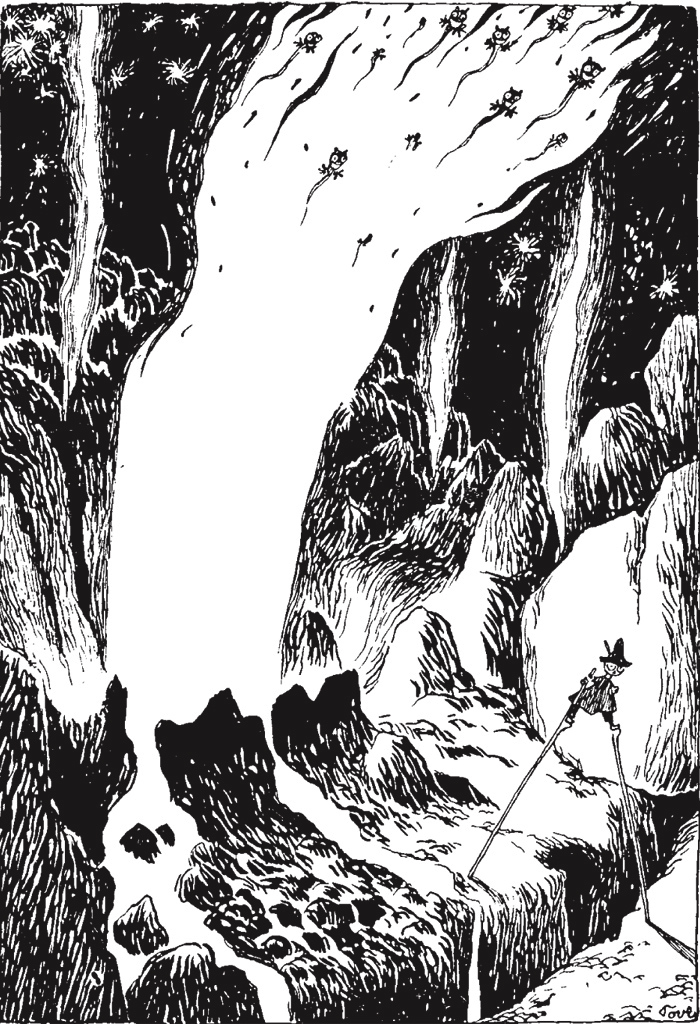
\includegraphics[width=450pt,height=660pt]{3-9.png}
\caption{}
\label{3-9}
\end{figure}

``Mi paŝis per stilzoj,'' diris Snufmumriko. ``Per stilzoj eblas paŝi sur ĉiaj ajn rokaj blokoj kaj abismoj. Sed kompreneble oni devas zorgi, ke ili ne fiksiĝu en fendo. Nu, mi trinkis mian teon en la plej malvarma loko, kiun mi trovis. Ĉie boletis kaj vaporis, kaj mi vidis eĉ ne unu vivulon aŭ verdan herbon. Kaj subite vekiĝis la tero kiu dormis tie sube. Per granda muĝado malfermiĝis kratero rekte antaŭ mi, kaj el ĝi ŝprucis ruĝa fajro kaj enormaj nuboj el cindro.''

``Fajrosputa monto!'' kriis Snif. ``Kion vi faris?''

``Mi nur rigardis,'' diris Snufmumriko. ``Ĝi estis ege bela. Mi vidis amason da fajro-spiritoj kiuj svarmis supren el la tero kaj disflugis kiel fajreroj. Post iom iĝis tro varmege kaj fulge, do mi ekiris de tie. Sube laŭ la monta deklivo mi trovis rivereton, kaj mi kuŝiĝis surventre por trinki. Kompreneble la akvo estis varma, sed ĝi ne bolis. Kaj tiam alflosis unu el tiuj fajro-spiritoj. Li enfalis kaj jam preskaŭ estingiĝis. Nur lia kapo plu ardis, la cetero siblis kaj fumis, kaj li kriis laŭ sia pleja kapablo ke mi savu lin.''

``Ĉu vi faris tion?'' demandis Snif.

``Jes ja, mi havis nenion apartan kontraŭ li. Sed mi bruliĝis tuŝante lin. Nu, li surteriĝis kaj iom post iom li ekbrulis denove. Kompreneble li ĝojis kaj donis al mi donacon antaŭ ol forflugi.''

``Kion do?'' ekkriis Snif.

``Boteleton da subtera sunoleo,'' diris Snufmumriko. ``Tion per kio la fajro-spiritoj ŝmiras sin kiam ili iros plej profunde en la mezon de la tero.''

``Kaj ĉu vi povas trairi fajron se vi surmetas tiun oleon?'' demandis Snif kun gapantaj okuloj.

``Certe,'' diris Snufmumriko.

``Kaj tion vi diras nur nun?'' vokis Mumintrolo. ``Do ni estas savitaj, ĉiuj. Kiam la kometo venos, ni simple prenos{\ldots}''

``Sed preskaŭ neniom restas al mi,'' malĝoje deklaris Snufmumriko. ``Komprenu, mi savis aĵojn el brulantaj domoj. Ja mi ne sciis{\ldots} Kaj nun restas nur eta kvanto surfunde de la botelo.''

``Ĉu ĝi eble sufiĉus por besteto de, ni diru --- mia grandeco?'' demandis Snif.

Snufmumriko rigardis lin.

``Eble,'' li diris. ``Sed apenaŭ la vosto. Tiun vi devus lasi forbruli.''

``Ĉu tiel,'' diris Snif. ``Tiuokaze prefere la tuto brulu. Sed ĉu ĝi do sufiĉos por katido?''

Sed Snufmumriko ne aŭskultis.

Li sidis kun rekta dorso kaj maltrankvile flaris.

``La rivero,'' li diris. ``Ĉu vi rimarkas ion?''

``Ĝi havas tute novan sonon,'' diris Mumintrolo.

Tio estis vera, la rivero susuregis kaj murmuris. Ĉie ĉirkaŭ ili troviĝis akvokirloj kaj ili ne plu estis etaj.

``Mallevu la velon,'' diris Snufmumriko.

La fluo jam estis tre forta. Nun la rivero ĵetiĝis antaŭen kvazaŭ iu, kiu post longa vojaĝo subite rimarkas, ke li preskaŭ venis hejmen. La bordoj alproksimiĝis, kaj super ili la montoj leviĝis pli kaj pli alte kaj akre.

``Mi pensas, ke mi volas surteriĝi,'' diris Snif.

``Ni ne povas surteriĝi,'' respondis Snufmumriko. ``Ni devas pluiri ĝis la rivero kvietiĝos.''

Sed ĝi tute ne kvietiĝis. La bordoj eĉ pli proksimiĝis kaj premis la ŝaŭman akvon en mallarĝa kanalo. Ili venis en Solecan Montaron. La floso kirliĝis antaŭen sube en profunda ravino, kaj la strio de ĉielo super ili iĝis pli kaj pli mallarĝa. Ie en la grundo io minace muĝis.

\begin{figure}[htbp]
\centering
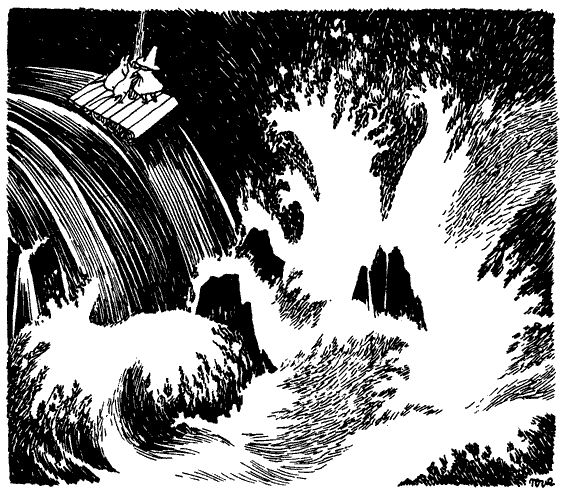
\includegraphics[width=425pt,height=372pt]{3-10.png}
\caption{}
\label{3-10}
\end{figure}

Mumintrolo rigardis Snufmumrikon por vidi, ĉu li timas. La mumriko ankoraŭ tenis la pipon enbuŝe, sed ĝi estingiĝis. Nigraj kaj malsekegaj de akvo la flankoj de la fendego preterflugis ilin, la muĝado plilaŭtiĝis, la floso skuiĝis, ĝi sagis en la aeron{\ldots}

``Fikstenu al io ajn ĉar nun ni iros suben!'' kriis Snufmumriko.

Dum kelkaj momentoj troviĝis nur ondegoj el blanka ŝaŭmo kaj muĝado de la rivero. Neniu aŭdis ke Snif kriegis. La eta floso krakis kaj alĝustiĝis post la akvofalo. Poste ĝi pluiris en mallumon.

``Kial estas mallume?!'' kriis Snif.

Neniu respondis.

La ŝaŭmanta akvo lumis blankverde, ĉio cetera estis nigra. La rokaj flankoj fermiĝis ĉirkaŭ ili kiel tunelo, kie la floso senpove pluiris tra la akvokirloj. De temp' al tempo ĝi puŝiĝis al la flankoj kaj turniĝis en rondo. La tondro de la akvofalo malantaŭ ili iom post iom mallaŭtiĝis, fine restis nur mallumo kaj silento ĉirkaŭ ili.

``Ĉu vi restas?'' tremante demandis Snif.

``Mi pensas ke mi restas,'' respondis Mumintrolo. ``Jen io por rakonti al Panjo!''

Nun eklumis malvasta strio de lumo, Snufmumriko trovis la poŝlampon. La lumo time flirtis sur nigra fluanta akvo kaj malsekaj muroj el ŝtono.

``Ŝajnas al mi, ke iĝas pli kaj pli malvaste,'' diris Mumintrolo per tre malgranda voĉo. ``Ĉu vi ne trovas, ke iĝas pli malvaste?''

``Eble iomete,'' respondis Snufmumriko kaj klopodis esti trankviliga. Sed li ne sukcesis. Poste ekkrakis, kaj la pinto de la masto falis sur la floson.

``Helpu min ĵeti la maston de la floso,'' vokis Snufmumriko. ``Sed rapide!''

La masto plaŭdis kaj malaperis en la akvon. Ili atendis, proksime premitaj unu al la alia. Subite Snif sentis ion froti liajn orelojn.

``Miaj oreloj!'' li kriis. ``Miaj oreloj tuŝis la plafonon!''

Li ĵetis sin surventre kaj metis la manojn super la nazon. Ĝuste tiam la floso skue haltis.

``Sidu senmove,'' diris Snufmumriko. ``Ne moviĝu.''

La tunelo estis plena de malfortega griza lumo, ili apenaŭ povis vidi la teruritajn vizaĝojn unu de la alia. Snufmumriko eklumigis la poŝlampon kaj rigardis suben en la akvon. Jen la masto, li diris. Ĝi kuŝiĝis transverse, kaj ni fiksiĝis sur ĝi. Rigardu, kion ni evitis!

Ili rigardis. Nigra brila akvo preterfluis, plufluis kaj poste malaperis kun terura gargara sono rekte suben ensenfundan truon.

``Nun mi laciĝis de vi kaj via vojaĝado kaj viaj kometoj kaj ĉio,'' ekkriis la besteto Snif kaj komencis plori. ``Mi ja diris, ke ĉi tio okazas je via risko. Mi ja diris ke mi volas surteriĝi! Kiam oni estas tiel malgranda kiel mi{\ldots}''

``Aŭskultu,'' diris Snufmumriko. ``Mi scias, ke en aventuraj historioj oni ĉiam saviĝas. Foje rigardu supren.''

Snif blovis la nazon permane kaj rigardis. Li vidis vertikalan fendegon en la roko kaj plej supre strion da griza ĉielo.

``Nu, kio do?'' li diris. ``Mi ne estas muŝo. Kaj se mi estus muŝo tio ne helpus min, ĉar mi kapturniĝas pro alteco jam de mia infanaĝo, kiam mi havis orelan inflamon.''

Kaj denove li ploris.

Tiam Snufmumriko elpoŝigis sian buŝharmonikon kaj ekludis. Li ludis la kanton pri aventuroj, kiuj ne estas konvene grandaj sed tute enormaj, kaj la rekantaĵo temis pri saviĝoj kaj surprizoj ĝenerale. Iom post iom

Snif trankviliĝis kaj sekigis siajn lipharojn. Sed la kanto flugis supren laŭ la fendego tra la roko, ĝi vekis unu eĥon post alia, kaj fine ĝi vekis hemulon kiu sidis dormante apud sia papilia kaptosako.

``Nu, jen kio?'' diris la hemulo kaj rigardis ĉirkaŭ si. Li rigardis supren al la ĉielo kaj en la kaptsakon kaj poste li deŝraŭbis la kovrilon de sia skaraba skatolo kaj rigardis ankaŭ en ĝin. ``Bruo,'' li diris. ``Jen estas io kio bruas (li ne komprenis muzikon).'' Fine la hemulo prenis sian grandigan lenson kaj ekserĉis inter la herboj. Li serĉis kaj aŭskultis kaj flaris kaj snufis kaj fine li atingis profundan fendon en la grundo. Tie estis terura bruo.

\begin{figure}[htbp]
\centering
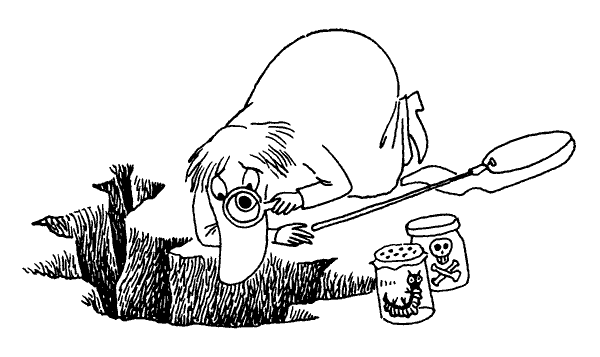
\includegraphics[width=350pt,height=206pt]{3-11.png}
\caption{}
\label{3-11}
\end{figure}

``Devas esti tre maloftaj insektoj,'' la hemulo diris al si. ``Certe tre raraj kaj eble eĉ nekonataj!''

La penso tre ekscitis la hemulon kaj li enigis sian grandan nazon en la fendon por pli bone vidi.

``Rigardu! Jen hemulo!'' kriis Mumintrolo.

``Savu nin! Savu nin!'' blekis Snif.

``Nun ili komplete ekscitiĝas,'' murmuris la hemulo kaj enŝovis sian kaptosakon. Ĝi estis ege peza kiam ĝi revenis supren. La hemulo haŭlis kaj haŭlis kaj poste li rigardis kion li ekhavis en ĝi.

``Tre strange,'' diris la hemulo kaj elskuis Mumintrolon, Snufmumrikon, Snif'on, tendon kaj du dorsosakojn.

``Grandan dankon,'' diris Mumintrolo. ``Vi savis nin en la lasta momento.''

``Ĉu mi savis vin?'' surprizite diris la hemulo. ``Mi ne intencis tion. Mi nur serĉis kelkajn rarajn insektojn, kiuj bruadis tie sube.''(Hemuloj ĝenerale malbone komprenas sed estas afablaj, se oni ne incitas ilin.)

``Ĉu ĉi tio estas Soleca Montaro?'' demandis Snif.

``Mi ne scias,'' respondis la hemulo. ``Sed troviĝas tre interesaj noktaj papilioj ĉi tie.''

``Jes, ĉi tio estas Soleca Montaro,'' diris Snufmumriko.

Ĉirkaŭ ili altiĝis grandega montaro, senfine dezerta kaj griza. Estis tre silente kaj la aero estis malvarmeta.

``Nu, kie troviĝas nia Observatorio,'' pluis Snif.

``Ankaŭ tion mi ne scias,'' diris la hemulo kaj komencis incitiĝi. ``Sed kion vi scias pri noktaj papilioj, tion mi scivolas.''

``Ni serĉas nur kometojn,'' diris Snif.

\begin{figure}[htbp]
\centering
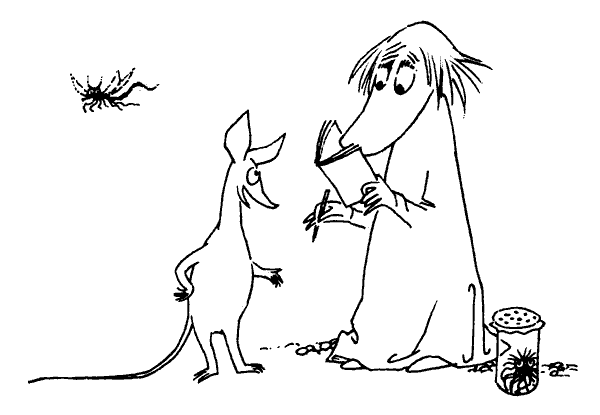
\includegraphics[width=349pt,height=241pt]{3-12.png}
\caption{}
\label{3-12}
\end{figure}

``Ĉu ili estas maloftaj?'' demandis la hemulo kun interesiĝo.

``Eblas diri ke jes,'' respondis Snufmumriko. ``Proksimume unu en cent jaroj.''

``Mirinde,'' diris la hemulo. ``Tian mi ŝatus kapti. Kiel ili aspektas?''

``Ruĝaj kaj kun longa vosto,'' diris Mumintrolo.

La hemulo elpoŝigis sian notlibron kaj notis tion.

``Devas esti la genro Filiknarkus Snufsigalonika,'' li murmuris. ``Ankoraŭ demando, miaj kleraj amikoj, kiel nutras sin tiu mirinda insekto?''

``Per hemuloj,'' diris Snif subridante.

La vizaĝo de la hemulo ruĝiĝis.

``Oni ne ŝercas pri la scienco,'' li diris. ``Adiaŭ. Mia riverenco.''

Poste li kolektis ĉiujn siajn skatolojn, prenis la papilian kaptosakon kaj foriris, rekte en Solecan Montaron.

``Li kredis ke la kometo estas skarabo aŭ similaĵo,'' ravite vokis Snif. ``Kiel ridinde! Kiel mirinde! Nun mi deziras kafon!''

``La kafokruĉo restas sur la floso,'' diris Snufmumriko. Mumintrolo, kiu amis kafon, kuris ĝis la fendo kaj rigardis suben.

``La floso malaperis!'' li kriis. ``La kafokruĉo iris subteren!''

Kiel ni vivu sen kafo?

``Ni manĝos krespetojn,'' diris Snufmumriko.

\begin{figure}[htbp]
\centering
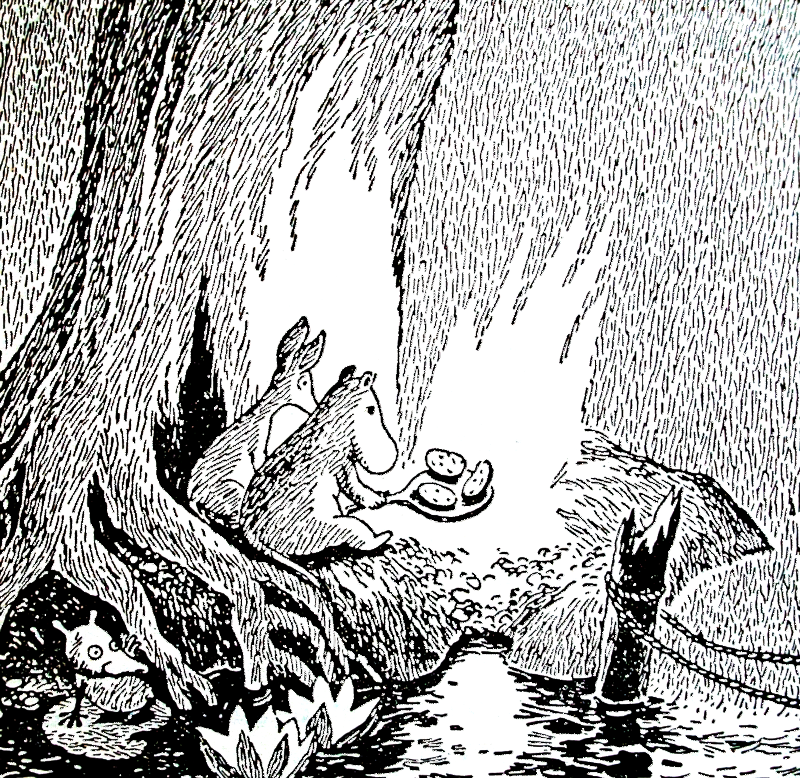
\includegraphics[width=439pt,height=427pt]{3-13.png}
\caption{}
\label{3-13}
\end{figure}

Do ili faris fajron kaj fritis krespetojn, kiujn ili manĝis unu post alia, laŭvice kiam ili pretiĝis, kio estas la sola ĝusta maniero manĝi krespetojn.

Kiam restis neniu, ili elektis la plej altan montaron kaj komencis malrapide marŝi supren kontraŭ la pinto. Ĉar se oni konstruas

Observatorion, sendube oni faras tion kiel eble plej proksime al la steloj.
\sectionbreak
Estis malfrue vespere. La pratempaj montoj staris solene revante, la pintoj rigardis unu la alian trans abismo, kie leviĝis nebuloj, grizblankaj kaj glacie malvarmaj. Jen kaj jen iu nubeto disiĝis el la pezaj nubaroj kaj malrapide glisis super la montoflanko, kie aglo kaj kondoro havis siajn nestojn.

Sub unu el la montopintoj brilis malgranda lumeto. Venante pli proksime oni povis vidi, ke ĝi estas flava tendo, lumigata de interne. La buŝharmoniko de Snufmumriko sonis tre soleca en la dezerta pejzaĝo, kaj tre malproksime hieno levis sian kapon aŭskultante. Ŝi neniam antaŭe aŭdis muzikon. Poste ŝi ululis, terure kaj longe.

``Kio estis tio?'' diris Snif kaj movis sin pli proksimen al la lumo.

``Nenio danĝera,'' diris Snufmumriko. ``Nun ni ludu tiun kanton pri burdo kiu iris al maskobalo.'' Kaj li denove ekludis.

``Jen bona kanto,'' diris Mumintrolo. ``Sed oni ne komprenis, kio okazis al la burdo kaj ĉu la maskobalo estis amuza. Prefere rakontu ion al ni.''

Snufmumriko dum kelka tempo cerbumis. Poste li demandis:

``Ĉu mi iam rakontis pri la snorkoj kiujn mi renkontis antaŭ kelkaj semajnoj?''

``Ne,'' diris Mumintrolo. ``Kio estas snorko?''

``Ĉu vi vere ne scias kio estas snorko?'' surprizite demandis Snufmumriko. ``Ja ili devas esti viaj parencoj, ĉar vi estas tute samaj. Kvankam kompreneble vi estas blanka, kaj ili estas buntaj kaj krome ili ŝanĝas koloron kiam ili ekscitiĝas.''

La okuloj de Mumintrolo ekhavis koleran mienon.

``Ni tute ne estas parencoj,'' li diris. ``Mi ne estas parenco de iu kiu ŝanĝas koloron. Troviĝas nur unu speco de mumintrolo, kaj ĝi estas blanka!''

``Ĉiuokaze tiuj snorkoj tre similis vin,'' trankvile diris Snufmumriko. ``Tio estas --- la konturoj. La snorko ŝatis ordigi kaj klarigi aferojn, tio ofte estis sufiĉe ĝena. Lia fratineto aŭskultis sed mi supozas ke ŝi pensis pri io alia. Eble pri si mem. Ŝi estis komplete kovrita de bela mola lanugo kaj havis fruntharojn, kiujn ŝi brosis senĉese.''

``Kiel stulte,'' diris Mumintrolo.

``Nu, kio poste okazis,'' demandis Snif.

``Ho, nenio aparta okazis,'' diris Snufmumriko. ``Ŝi teksis etajn dormomatojn el herboj kaj kuiris bonfarajn supojn se oni havis stomakdoloron. Plue ŝi portadis florojn malantaŭ la oreloj kaj oran ringon ĉirkaŭ la maldekstra piedo.''

``Sed ĉi tio ja ne estas historio,'' vokis Snif. ``Entute neniu ekscito!''

``Ĉu vi ne trovas ekscite unuafoje en la vivo vidi snorkon, kiu krome povas ŝanĝi koloron?'' demandis Snufmumriko kaj plu ludis.

``Fraŭlinoj estas stultaj kaj ankaŭ vi,'' diris Mumintrolo kaj enrampis en la dormsakon turnante la nazon al la tendotuko.

Sed tiunokte li sonĝis pri eta snorkfraŭlino kiu similis lin mem kaj al kiu li donis rozon por porti malantaŭ la orelo.

\begin{figure}[htbp]
\centering
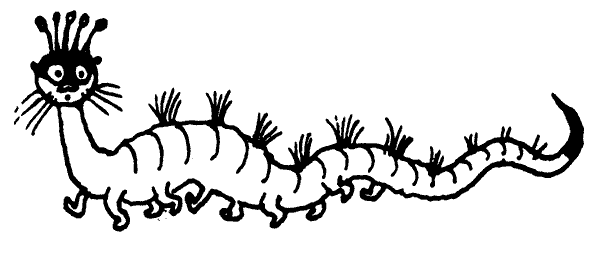
\includegraphics[width=150pt,height=66pt]{3-14.png}
\caption{}
\label{3-14}
\end{figure}

\chapter*[Ĉapitro 4]{Ĉapitro 4}
\addcontentsline{toc}{chapter}{Ĉapitro 4}


\begin{figure}[htbp]
\centering
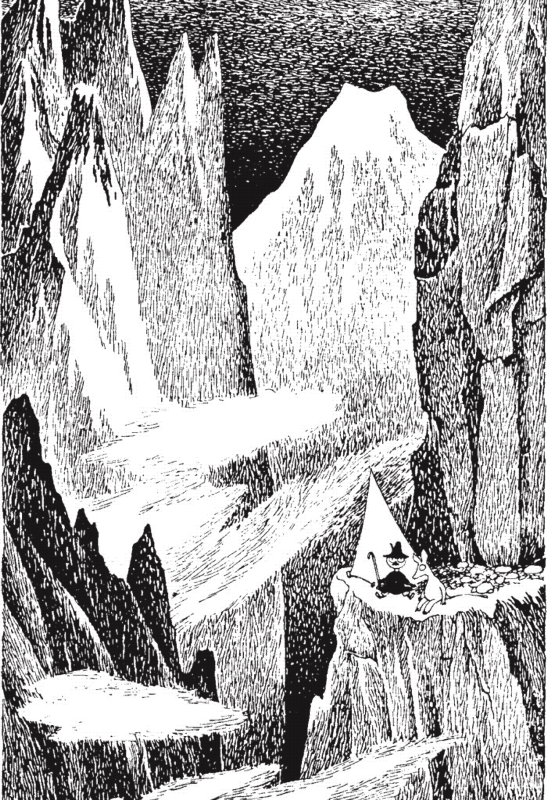
\includegraphics[width=450pt,height=655pt]{4-1.png}
\caption{}
\label{4-1}
\end{figure}

``Kiel stulte,'' diris Mumintrolo, kiam li matene vekiĝis. ``En la tendo estis glacie malvarme.''

Snufmumriko ĝuste kuiris teon.

``Hodiaŭ ni supreniru sur la plej altan pinton,'' li diris.

``Kaj kiel vi scias, ke ĝi estas la ĝusta,'' demandis Snif, streĉante la kolon por ekvidi la pinton. Sed ĝi estis kaŝita trans pezaj grizaj nuboj.

``Rigardu tion,'' respondis Snufmumriko. ``Ĉie kuŝas cigaredstumpoj! La profesoroj ĵetis ilin suben.''

``Ho, ĉu vere,'' diris Snif embarasite pro tio ke li mem ne eltrovis tion.

Ili piediris supren laŭ serpentuma monta pado, kaj inter ili troviĝis savŝnuro kiun ili nodis ĉirkaŭ la ventron por esti sekuraj.

``Memoru ke nun refoje ĉio okazas je via risko,'' diris Snif, kiu iris la lasta. ``Kaj pensu pri mia orelinflamo.''

Iĝis pli kaj pli krute, ili venis pli kaj pli alten. Ĉio ĉirkaŭ ili estis pratempa, giganta kaj soleca, terure soleca.

Inter la nudaj krutaĵoj kondoro ŝvebis sur etenditaj flugiloj, li estis la sola vivulo videbla.

``Kia grandega birdo,'' diris Snif. ``Kiel soleca li devas esti tie supre!''

``Li sendube ie havas edzinon kaj eble tutan vicon da kondoridetoj,'' diris Snufmumriko.

\begin{figure}[htbp]
\centering
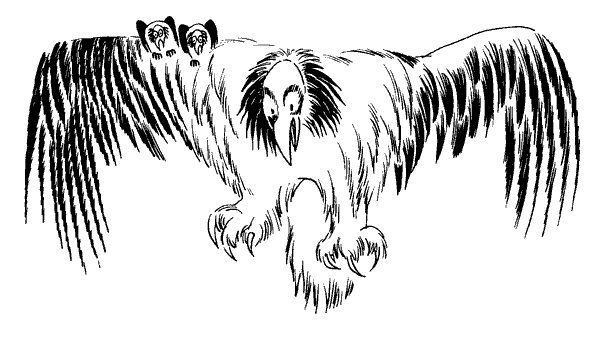
\includegraphics[width=284pt,height=160pt]{4-2.png}
\caption{}
\label{4-2}
\end{figure}

La kondoro digne glisis plu, li turnis sian kapon kun la malvarmaj okuloj kaj la kurba beko tien-reen. Precize super ili li haltis kun tremantaj flugiloj.

``Pri kio li nun cerbumas?'' scivolis Snif.

``Li aspektas kolera,'' diris Mumintrolo. ``Mi pensas ke li cerbumas pri ni{\ldots}''

Kaj tiam kriis Snufmumriko: ``Li venas!''

Kaj ĉiuj tri ĵetis sin kontraŭ la rokan flankon. Dum muĝado de flugiloj la kondoro faligis sin al ili. Ili kune premis sin en etan fendon en la roko, firme tenis unu la alian kaj atendis en senpova teruriĝo. Jen li venis! Li alflugis kiel ŝtormo, la enormaj flugiloj batis al la roko kaj ĉirkaŭ ili iĝis mallume, estis terure!

Kaj jen subite ĉio denove estis kvieta. Tremante ili eligis la nazojn.

Fore sub ili en la pli kaj pli malhela abismo la kondoro ŝvebis en granda duoncirklo. Poste li rapide altiĝis kaj pluflugis inter la montojn.

``Li hontas ke tio ne prosperis al li,'' diris Snufmumriko. ``Kondoroj estas tre fieraj. Li sendube ne reprovos tion.''

``Li kun siaj etaj kondoridoj!'' ekscitite kriis Snif. ``Tre kortuŝe! Kaj gigantaj saŭroj! Akvofaloj kiuj eniĝas senpere en la teron!''

Estas tro multaj aventuroj por tia besteto kiel mi!

``Restas al vi la plej granda aventuro,'' diris Mumintrolo. ``Nia kometo.''

La triopo rigardis supren al la pezaj nuboj.

``Mi preferus vidi la ĉielon,'' diris Snufmumriko. Li levis plumon kiun la kondoro postlasis kaj metis ĝin sur sian ĉapelon. ``Venu,'' li diris. ``Ni devas pluiri.''

Posttagmeze ili jam grimpis tiel alten ke ili eniris la nubojn. Subite ĉirkaŭis ilin nur malvarma nebulo, nenio krom griza malpleno. La monto estis glita kaj danĝera por suriri. Ili terure frostis, kaj Mumintrolo malĝoje pensis pri sia lana kalsono, kiu ĝuste nun survojis al la centro de la tero.

``Mi kredis ke nuboj estas molaj kaj lanaj kaj agrablaj por suriri,'' diris Snif ternante. ``Mi ege tediĝas de ĉi tiu tuta stulta vojaĝo!''

``Kio estas tio?'' diris Mumintrolo subite haltante. ``Jen kuŝas io brilanta{\ldots}''

``Ĉu diamanto?'' demandis Snif kaj vigliĝis.

``Ŝajnas al mi ke estas eta brakĉeno,'' diris Mumintrolo.

Li iris rekte en la nebulon.

\begin{figure}[htbp]
\centering
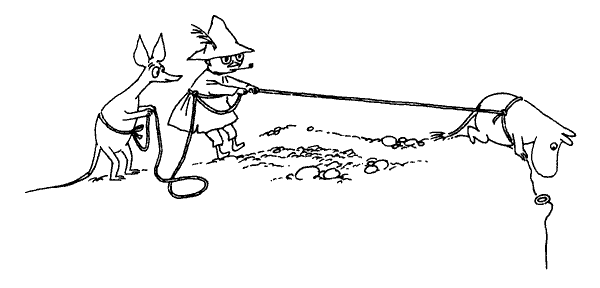
\includegraphics[width=200pt,height=96pt]{4-3.png}
\caption{}
\label{4-3}
\end{figure}

``Atentu,'' vokis Snufmumriko. ``Ĝi kuŝas ĝuste surrande de la abismo!''

Mumintrolo plupaŝis, ege singarde. Li kuŝiĝis surventre plej fore ĉe la abismo kaj etendis sian manon.

``Fikstenu la ŝnuron!'' li kriis.

Snufmumriko kaj Snif fikstenis plenforte, kaj la trolo eĉ pli klinis sin trans la randon. Fine li kaptis la brakĉenon kaj krablis reen.

``Ĝi estas el oro,'' li diris. ``Ĉu vi ne diris ke tiu snorkfraŭlino portis oran ringon ĉirkaŭ la maldekstra piedo?''

``Jes,'' diris Snufmumriko malgaje. ``Kaj kiel bela ŝi estis! Ŝi ĉiam volis iri en danĝerajn lokojn por pluki florojn.''

``Nun ŝi sendube iĝis kaĉo,'' diris Snif.

Ili melankolie marŝis plu, pli kaj pli alten kaj senĉese iĝis pli lacaj kaj malvarmaj. Fine ili sidiĝis por ripozigi la krurojn kaj silente gapis en la ondantajn grizajn vualojn.

Kaj jen ŝiraĵo malfermiĝis tra la nuboj. Subite la tuta nubaro kuŝis sub ili. De ĉi-supre ĝi aspektis mole kaj bele, oni ekemis vadi en ĝin, plonĝi kaj danci.

``Nun ni estas super la nuboj,'' solene diris Snufmumriko.

\begin{figure}[htbp]
\centering
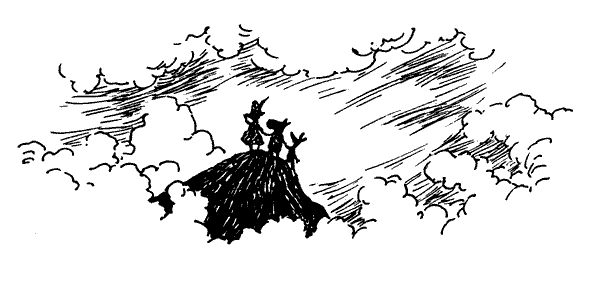
\includegraphics[width=350pt,height=165pt]{4-4.png}
\caption{}
\label{4-4}
\end{figure}

Kaj ili turnis sin kaj rigardis supren al la ĉielo, kiun ili jam delonge ne vidis.

``Kio estas tio?'' flustris Snif kun teruriĝo.

La ĉielo ne plu estis blua. Ĝi havis pale ruĝan koloron, kiu ne ŝajnis natura.

``Eble tio estas la sunsubiro,'' malcerte diris Snufmumriko.

``Jes ja, nature,'' diris Mumintrolo. ``La suno subiras.''

Sed ili sciis, ke tio ne estas la sunsubiro. Tio estis la kometo, kiu verŝis sian ruĝan lumon sur la vesperan ĉielon. Ĝi survojis al la tero kaj al ĉiuj bestoj vivantaj sur la tero.
\sectionbreak

\begin{figure}[htbp]
\centering
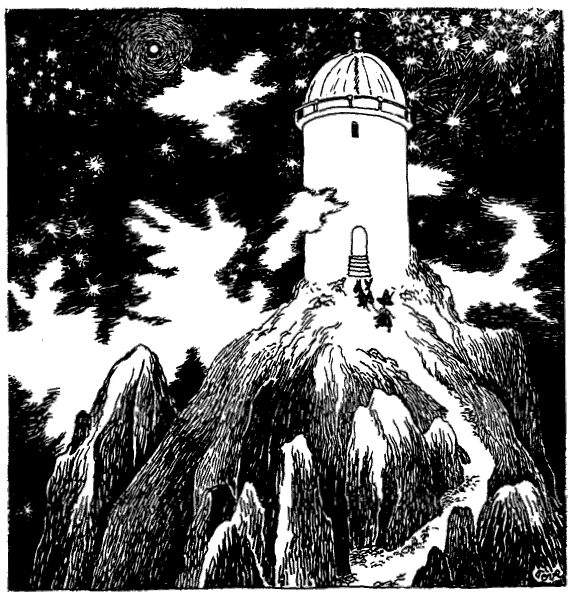
\includegraphics[width=443pt,height=462pt]{4-5.png}
\caption{}
\label{4-5}
\end{figure}

Plej alte sur la denta montaro situis la observatorio, kie profesoroj faris mil mirindajn observojn kaj fumis mil cigaredojn kaj vivis solece kun la steloj. La turo havis rondan vitran tegmenton kaj estis ornamita per ĉielarke bunta vitra globo. Ĝi senĉese rotaciis, malrapidege.

Mumintrolo iris antaŭ la aliaj. Li malfermis la pordegon kaj mirante haltis sur la sojlo. La tuta turo estis unu sola ĉambro kie la plej granda lorno senĉese rigardis la stelojn. Ĝi malrapide moviĝis rigardante en la spacon serĉante danĝerojn, kaj ĝi ronronis al si kiel kato.

Amaso da etaj profesoroj ĉie kuretis en rondoj, ili grimpis supren-suben laŭ ŝtuparoj el brila latuno, ili ŝraŭbis kaj mezuris kaj alĝustigis kaj jen kaj jen skribis en siaj notlibroj. Ili estis tre urĝataj kaj ĉiuj fumis cigaredojn.

``Bonan vesperon,'' diris Mumintrolo.

Sed neniu rimarkis lin. Tiam li singarde antaŭiris kaj tiris la kitelon de la plej proksima profesoro.

``Ĉu refoje vi estas ĉi tie,'' diris la profesoro.

``Pardonu, sed mi neniam antaŭe estis ĉi tie,'' timide deklaris

Mumintrolo.

``Do estis iu ege simila al vi,'' diris la profesoro. ``Neniu paco nuntempe. Ni ne havas tempon por uloj kiujvenadas por fari infanecajn demandojn. Piedringoj, je mia vosto. Ĉi tiu kometo estas la plej interesa afero kiu okazis al mi en mia tuta vivo{\ldots} Kion vi volas?''

``Nenion gravan,'' murmuris Mumintrolo. ``Mi nur ŝatus scii, ĉu ŝi estis lanuga{\ldots} tio estas tiu, kiu estis ĉi tie antaŭ mi --- eble ŝi portis floron malantaŭ la orelo?''

La profesoro levis siajn manojn ĉielen, suspirante.

``Lanugo kaj floroj ne interesas min,'' li diris. ``Ankaŭ ne piedringoj. Ĉu vi vere kredas ke tio ion signifas, se iu fraŭlino perdas sian piedringon, dum oni atendas kometon?''

``Tio eble ion signifas,'' serioze respondis Mumintrolo.

\begin{figure}[htbp]
\centering
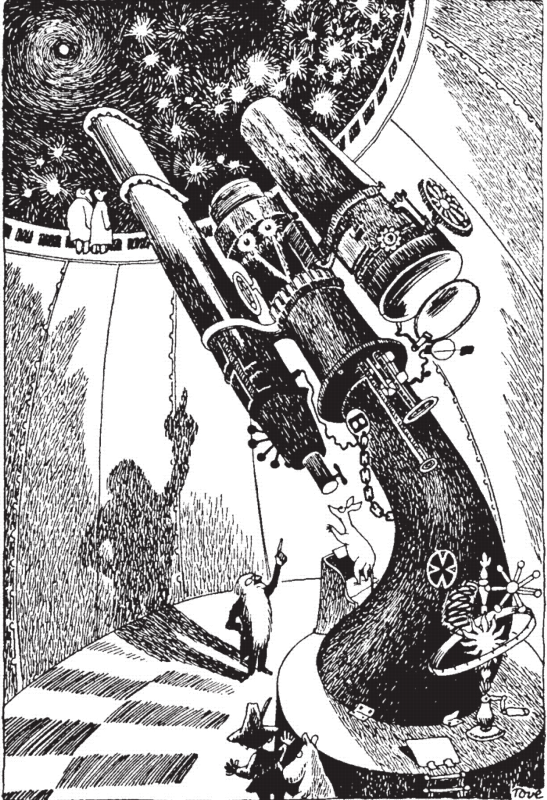
\includegraphics[width=450pt,height=658pt]{4-6.png}
\caption{}
\label{4-6}
\end{figure}

``Koran dankon.''

``Ne dankinde,'' diris la profesoro kaj plandis for al sia stelo-lorno.

``Nu, kion li diris?'' flustris Snif. ``Ĉu la kometo venos?''

``Kiam ĝi trafos la teron?'' demandis Snufmumriko.

``Mi forgesis demandi pri tio,'' diris Mumintrolo. ``Sed Snorkfraŭlino estis ĉi tie! Ŝi tute ne falis en la abismon!''

``Vi estas ridinda,'' diris Snif. ``Nun mi iras demandi. Vi povas rigardi dum mi ordigos la aferon.''

Kaj la besteto Snif iris ĝis alia profesoro kaj diris: ``Mi aŭdis amason pri kiel lerte vi trovas kometojn, onklo!''

``Ĉu vere?'' diris la profesoro kaj feliĉiĝis. ``Ĉi tio estas nekutime bela kometo. Mi pripensas ĉu eble nomi ĝin laŭ mi mem. Venu rigardi ĝin iomete.''

Snif postiris laŭ ĉiuj ŝtuparoj. Li estis la unua besteto kiu rajtis rigardi tra la plej granda lorno de la mondo.

``Nu, ĉu ĝi ne estas bela kometo?'' demandis la profesoro.

``La universo estas nigra. Ĝi estas tute nigra,'' flustris Snif. Li tiel timis, ke liaj nukaj haroj stariĝis. Meze de la nigro spiris la grandaj steloj kvazaŭ ili estus vivaj. Ili estis same grandaj kiel diris la moskorato. Kaj fore inter ili brilis io ruĝa kvazaŭ malica okulo.

``Jen la kometo,'' diris Snif. ``Tiu ruĝo estas la kometo, kaj ĝi venos ĉi tien.''

``Kompreneble ĝi venos ĉi tien,'' konsentis la profesoro.

``Jen la interesa afero. Ĉiutage ni povos vidi ĝin pli bone. En ĉiu tago kiu pasos ĝi iĝos pli kaj pli ruĝa kaj bela!''

``Sed ĝi restas senmova,'' diris Snif. ``Kaj mi ne vidas ke ĝi havas voston.''

``Ĝi havas la voston malantaŭe,'' klarigis la profesoro. ``Ĝi venas rekte kontraŭ ni, kaj tial ĝi ŝajnas senmova. Ĉu ĝi ne estas bela?''

``Nu,'' diris Snif. ``Ruĝo ja estas impona, klare. Kiam ĝi alvenos ĉi tien?'' Li gapis sorĉita de timo al la eta ruĝa fajrero en la lorno.

``Laŭ mia kalkulado ĝi tanĝos la teron la sepan de aŭgusto je la oka kvardek du vespere. Eventuale kvar sekundojn pli malfrue,'' respondis la profesoro.

``Kaj kio okazos tiam?'' demandis Snif.

``Kio okazos?'' diris la profesoro. ``Mi ne havis tempon pensi pri tio. Sed mi tre zorge notos la sinsekvon de eventoj.''

Snif komencis per tremaj kruroj grimpi suben laŭ la ŝtuparo. Duonvoje li subite haltis por demandi: ``Kiu tago estas hodiaŭ?''

``La trian de aŭgusto,'' respondis la profesoro. ``Kaj la horloĝo montras precize 19.53.''

``Do mi pensas ke ni devas hejmeniri,'' diris Snif. ``Ĝis revido!''

La besteto Snif estis rimarkeble pli granda kiam li revenis al la cetera duopo.

``Ĝi estas nigra,'' li diris. ``Karbe nigra.''

``Kio?'' demandis Mumintrolo.

``La universo, kompreneble,'' klarigis Snif. ``Kaj la kometo estas ruĝa kaj havas la voston malantaŭ si. Kaj ĝi intencas TANĜI la teron la sepan de aŭgusto je la oka kvardek du vespere. Eventuale kvar sekundojn pli malfrue. La profesoro kaj mi kalkulis tion.''

``Do ni devas rapidi hejmen,'' diris Mumintrolo. ``Kiu grava afero okazos dimanĉe?''

``Anĝelkaĉo,'' neglekteme diris Snif. ``Pura infanaĵo. Almenaŭ por iu kiu rigardis tra stelo-lorno.''

``Tamen ni devas rapidi,'' murmuris Mumintrolo. Li malfermis la pordon kaj kuris eksteren.

``Kvietiĝu,'' vokis Snufmumriko. ``Se ni kuros tiel, ni stumblos kaj falos en iun abismon. La kometo ja alvenos nur post kvar tagoj!''

``Kometo kaj kometo,'' ekkriis Mumintrolo. ``Sendube Paĉjo kaj''

Panjo zorgos pri ĝi se ni nur venos hejmen{\ldots} Sed ni devas trovi Snorkfraŭlinon! Ŝi ja ne scias ke mi trovis ŝian piedringon!

Li malaperis en la krepuskon kaj tiris la ceteran duopon post si per la ŝnuro. La terura ruĝeca koloro de la ĉielo intensiĝis. La nuboj fordrivis kaj la tuta montara pejzaĝo kuŝis nuda en la malrealeca vespera lumo.

Malproksime oni videtis la mallarĝan rubandon de la rivero kaj malhelajn makulojn el arbaro.

`Nu,' pensis Snufmumriko. `Estos plej bone se ili rajtos iri hejmen. Kaj supozeble snorkfraŭlino kun piedringo estas pli bona ol senringa, ĉu la kometo venos aŭ ne.'

\chapter*[Ĉapitro 5]{Ĉapitro 5}
\addcontentsline{toc}{chapter}{Ĉapitro 5}


La kvaran de aŭgusto ne plu estis nube, sed la sunon kovris stranga ombro. Dum kelka tempo ĝi ŝajnis nigra, ĝuste ruliĝante supren trans Soleca Montaro kaj ekglisante en la ruĝan ĉielon. Estis pli varme. Dum la tuta nokto ili nur marŝis kaj marŝadis. Snif komencis ĝemi.

``Mi estas laca,'' li diris. ``Mi laciĝis de la tuto. Nun estas via vico porti la tendon. Kaj la krespeto-paton.''

``Ĝi estas bona tendo,'' diris Snufmumriko. ``Sed oni evitu tro multe ŝati posedaĵojn. Simple forĵetu ĝin. Ankaŭ la krespeto-paton.''Tamen restas al ni nenio por meti sur ĝin.

``Ĉu vi vere intencas tion?'' konsternite demandis Snif. ``Suben en la abismon?''

Snufmumriko kapjesis.

Snif iris ĝis la krutaĵo.

``Eblus loĝi en ĝi,'' li murmuris. ``Mi povus ricevi ĝin kaj havi ĝin kiel mian propran tendon ĝis mi mortos{\ldots} kara mumintrolo, nun mi tute ne scias kion fari!''

``Vi ja havas la groton,'' Mumintrolo amike diris.

Tiam la besteto Snif ridis kaj ĵetis la tutan pakaĵon foren. Ĝi faris grandegajn saltojn inter la rokaj pintoj, la krespeto-pato tintis kiel fanfaro.

\begin{figure}[htbp]
\centering
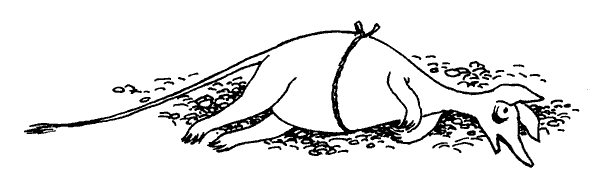
\includegraphics[width=350pt,height=105pt]{5-1.png}
\caption{}
\label{5-1}
\end{figure}

``Belege!'' kriis Mumintrolo, kaj igis la kaserolojn postsekvi. Ili faris eĉ pli belan bruon. Daŭris longe ĝis la lasta kaserolo silentiĝis sube en la abismo.

``Ĉu vi nun pli bone fartas?'' demandis Snufmumriko.

``Ne,'' diris Snif kaj iĝis tute palvizaĝa. ``Nun mi ekhavis kapturnon!'' Kaj li kuŝiĝis sternite sur la tero rifuzante pluiri.

``Aŭskultu,'' diris Mumintrolo. ``Ni devas rapidi. Mi devas kiel eble plej rapide trovi la etan{\ldots}''

``Mi scias, mi scias,'' interrompis Snif. ``Vian stultan Snorkfraŭlinon. Sed ne tuŝu min ĉar tiam mi vomos!''

``Lasu lin malbonfarti en paco,'' diris Snufmumriko. ``Atendante ni rulu iom da ŝtonoj. Ĉu vi iam rulis ŝtonojn?''

``Ne,'' diris Mumintrolo.

Snufmumriko elektis grandegan blokon kiu kuŝis ĝuste apud la roka rando.

``Nun rigardu,'' li diris kaj ekbalancis la ŝtonon, ``unu, du, tri'' kaj ĝi malaperis trans la randon. Ili kuris antaŭen por rigardi. Jen la bloko dancis antaŭen kvazaŭ fulmotondrus, ŝtonetoj ŝprucis kaj longe poste muĝantaj eĥoj ĵetiĝis tien-reen inter la montoflankoj.

``Fariĝis ŝtonlavango,'' feliĉe diris la mumriko.

``Ĉu ankaŭ mi!'' vokis Mumintrolo kaj kuris ĝis eĉ pli granda bloko kiu staris ekvilibre plej fore rande de la abismo.

``Singarde!'' kriis Snufmumriko.

Sed estis tro malfrue, la bloko tondre falis, kaj post ĝi flugis la malfeliĉa mumintrolo.

Nun verŝajne troviĝus je unu mumintrolo malpli en la mondo, se li ne havus la savŝnuron ĉirkaŭ la ventro. Snufmumriko tuj ĵetis sin dorsen kaj serĉis piedapogon por kontraŭi la puŝon. Ĝi estis forta puŝo, li sentis kvazaŭ li disduiĝus.

Sube en la abismo Mumintrolo senpove svingiĝis tienreen, kaj li estis sufiĉe peza trolo. Snufmumriko malrapide glitis pli kaj pli proksimen al la krutaĵo. La ŝnuro inter li kaj Snif streĉiĝis kaj ankaŭ Snif estis kuntirata sur la tero.

\begin{figure}[htbp]
\centering
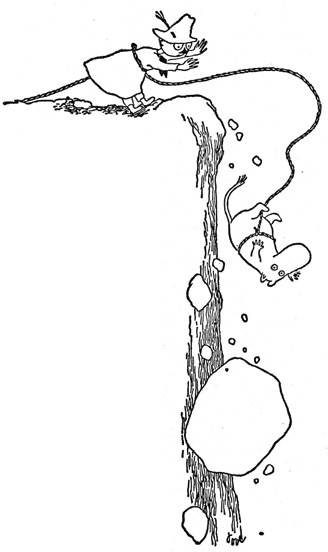
\includegraphics[width=180pt,height=302pt]{5-2.png}
\caption{}
\label{5-2}
\end{figure}

``Lasu,'' li ĝemis. ``Ne ĝenu min, mi malbonfartas{\ldots}''

``Vi eĉ pli malbonfartos kiam vi falos en la abismon post kelka tempo,'' diris Snufmumriko. ``Fikstenu kaj tiru! Kaj sube Mumintrolo blekis:''

``Helpon! Tiru min supren!''

Snif levis la nazon, kaj lia vizaĝo eĉ pli verdiĝis, sed ĉifoje tio estis pro teruriĝo. Li provis forrampi, li apogis sin mane, piede kaj voste, li glitis tien-reen, kaj kiel ajn li baraktis, la ŝnuro implikiĝis inter la rokoj kaj ili ĉesis gliti.

``Kaj nun tiru,'' diris Snufmumriko. ``Haŭlu per via plena forto kiam mi diras `nun'. Tio estas --- ne nun. Ne nun. Sed nun!'' Kaj jen ili tiris plenforte, pecon post peco, kaj finfine vidiĝis Mumintrolo super la rando. Unue la oreloj, poste la okuloj, poste la nazo, poste ankoraŭ pli da nazo kaj fine la tuta mumintrolo.

``Je mia vosto,'' li diris. ``Ĉi tion Panjo devus sperti.''

``Saluton!'' diris Snif. ``Bone revidi vin. Mi estas tiu, kiu igis ĉion halti!''

Ili longe sidis por trankviliĝi. Subite Mumintrolo diris: ``Ni estis stultaj.''

``Certe vi estis tiaj,'' diris Snif.

``Nepardoneble,'' pluis Mumintrolo. ``Krime! Imagu se ni rulis tiujn ŝtonojn sur la kapon de eta Snorkfraŭlino!''

``Tiuokaze ŝi nun estas plata,'' diris Snif.

Mumintrolo salte stariĝis.

``Ni devas pluiri,'' li ekkriis. ``Tuj!''

Kaj sub la malintense ruĝa ĉielo kun ĝia pala sundisko ili pluiris malsupren.
\sectionbreak
Sub la monto fluis rivereto inter la ŝtonoj. Ĝi estis tre malprofunda kaj havis oran glimon sur sia fundo. La hemulo sidis kun siaj lacaj piedoj en la akvo suspirante al si mem. Apude li havis dikan libron titolitan «Insektoj de la Norda Duonsfero, iliaj Kutimoj kaj Fikutimoj».

``Strange,'' diris la hemulo. ``Eĉ ne unu sola kun ruĝa vosto. Se ne temus pri Dideroformia Fnatopogetes, sed ĝi estas tre ofta kaj havas neniun ajn voston.''

Kaj li refoje suspiris.

\begin{figure}[htbp]
\centering
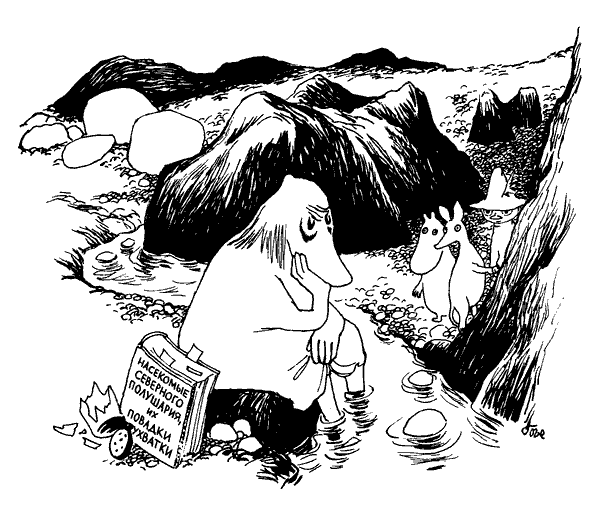
\includegraphics[width=349pt,height=297pt]{5-3.png}
\caption{}
\label{5-3}
\end{figure}

``Saluton,'' diris Mumintrolo kaj aperis de malantaŭ angulo de roko.

``Uf, kiel mi ektimis,'' diris la hemulo. ``Jen vi denove. Mi kredis ke vi estas ŝtonlavango. Ĉi-matene estis tute terure.''

``Kio?'' demandis Snif.

``La ŝtonlavango, kompreneble,'' respondis la hemulo. ``Tute terure. Ŝtonoj grandaj kiel domoj saltadis ĉie kaj rompis mian plej grandan vitran skatolon. Ankaŭ mi saltis. Rigardu la ŝvelaĵon sur mia kapo! Nur rigardu ĝin!''

``Mi bedaŭras, ke ni hazarde ĵetis kelkajn ŝtonojn suben, preterpasante,'' diris Snufmumriko. ``Estas malfacile rezigni, se ili estas tre grandaj kaj rondaj{\ldots}''

``Ĉu vi volas diri, ke ĝi estis via ŝtonlavango?'' malrapide demandis la hemulo. ``Mi devus diveni tion. Kompreneble. Efektive mi neniam trovis vin tre simpatiaj, kaj post tio ĉi estas necerte ĉu mi volas plu koni vin.''

Kaj li turnis sin for verŝante akvon sur siajn lacajn piedojn. Post kelka tempo li diris: ``Ĉu vi ankoraŭ ne foriris?''

``Ni baldaŭ ekiros,'' respondis Snufmumriko. ``Ni nur ŝatus scii, ĉu vi rimarkis ion strangan pri la koloro de la ĉielo.''

``Koloro de la ĉielo?'' la hemulo surprizite ripetis.

``Jes, la ruĝa koloro.''

``Aŭskultu,'' diris la hemulo. ``La ĉielo povas esti kvadratita se ĝi volas, en ordo laŭ mi. Mi maloftege rigardas ĝin. Kio zorgigas min estas ke mia bela rivereto senakviĝas. Se tio ĉi daŭros, mi ne plu povos plaŭdi per la piedoj.''

``Sed estas granda danĝera kometo,'' ekis Mumintrolo. Tiam la hemulo stariĝis, kolektis siajn aferojn kaj vadis ĝis la transa flanko.

``Venu, ni iru,'' diris Snufmumriko. ``Sendube li preferas esti sola.''

La tero iĝis pli agrabla por surtreti, ĝi estis kovrita de likenoj kaj muskoj kaj jen kaj jen kreskis kelkaj floroj. La arbaro alproksimiĝis.

Estis varmege.

``En kiu direkto vi loĝas?'' demandis Snufmumriko. ``Ĉar nun ni devos iri laŭ rekta vojo por veni tien antaŭ la kometo.''

Mumintrolo rigardis la kompason.

``Ĝi tute freneziĝis,'' li diris. ``Ĝi nur turniĝas en rondo. Ĉu vi pensas ke ĝi timas la kometon?''

``Tio eblas,'' diris Snufmumriko. ``Ni devos iri intue. Mi ĉiuokaze neniam kredis je kompasoj. Ili nur detruas la naturan senton pri direktoj.''

``Ĝuste nun mi havas naturan senton pri manĝo,'' informis Snif. ``Kial ni jam delonge ne manĝas?''

``Ĉar la manĝo elĉerpiĝis,'' diris Snufmumriko. ``Trinku fruktsukon kaj provu pensi pri io agrabla.''

Post iom ili venis al lageto. Ĝia akvo malaltiĝis al malprofunda flako kiu fiodoris, kaj ĉe la bordoj algoj malfreŝis, verdaj kaj ŝlimaj. Ĝi ne plu estis ĉarma lago por banoj.

``Eble ĝia fundo truiĝis,'' diris Snif. ``Kaj nun ĉiu akvo elfluas.''

``Ankaŭ la rivereto de la hemulo malaltiĝis,'' diris Mumintrolo.

Snif rigardis en la fruktsuka botelo.

``Ankaŭ ĉi tie malaltiĝis!'' li kriis.

``Ej,'' diris Mumintrolo. ``Vi mem trinkis el ĝi. Ne estu azeno.''

``Vi estas azeno!'' kriis Snif, ĉar li laciĝis kaj timis kaj malsatis, kaj ĝuste tiam ili aŭdis iun alvoki helpon. Iu kriis en la arbaro. Estis tre laŭtaj kaj ŝiraj krioj, kiuj levis la nukajn harojn de la tuta triopo. Mumintrolo ekkuris kiel kanonkuglo.

``Atendu!'' kriis Snif. ``Mi ne povas sekvi! Ho! Aj!'' La savŝnuro streĉiĝis ĉirkaŭ lia ventro, li falis survizaĝen kaj blekante estis tirata plu laŭ la tero. Sed la aliaj ne haltis, ĝis ili kuris ambaŭflanke de arbo kaj falis teren.

``Forigu la morhan ŝnuron!'' kolere diris Mumintrolo.

``Vi sakris!'' diris Snif.

``Ĉu gravas?'' reciproke kriis la trolo. ``Estas Snorkfraŭlino, kiu alvokas helpon! Mi scias, ke estas ŝi!''

``Nun vi ambaŭ trankviliĝu,'' diris Snufmumriko. Li eligis sian tranĉilon kaj distranĉis la ŝnuron.

Denove Mumintrolo ekkuris tiel rapide kiel li povis per siaj mallongaj kruroj. Post kelka distanco li renkontis la snorkon, kiu bluiĝis pro teruro kaj kriis: ``Terura arbedo manĝas mian fratinon!''

Kaj li tute pravis.

Venena arbedo de la danĝera genro Angosturo kaptis la voston de Snorkfraŭlino kaj malrapide tiris ŝin al si per siaj vivaj brakoj, dum ŝi, tre kompreneble, estis violkolora pro timego kaj kriis pli laŭte ol iu snorkfraŭlino iam ajn kriis.

``Mi venas! Mi venas!'' vokis Mumintrolo.

``Prenu ĉi tiun pro sekuro,'' diris Snufmumriko kaj donis al li sian tranĉilon (tiun kun korktirilo kaj ŝraŭbilo). ``Kaj provu kolerigi ĝin. La angosturoj tre facile ofendiĝas.''

\begin{figure}[htbp]
\centering
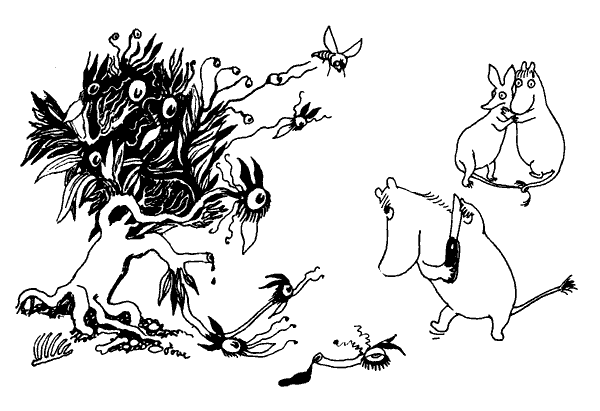
\includegraphics[width=400pt,height=274pt]{5-4.png}
\caption{}
\label{5-4}
\end{figure}

``Ter-rampanto! Lavbroso!'' vokis Mumintrolo. La angosturo ne reagis.

``Pispot-broso!'' kriis la trolo. ``Aĉa ratvost-pesto! Vi ŝajnas koŝmaro post tagmanĝo el memmortinta porko!''

Tiam la angosturo turnis ĉiujn siajn verdajn okulojn al li kaj lasis Snorkfraŭlinon. Unu el la longaj brakoj etendiĝis kiel serpento kaj volviĝis ĉirkaŭ la nazo de Mumintrolo.

``Rezistu!'' kriis Snufmumriko.

``Pedikaĉo!'' blekis la trolo, kaj trinĉ tranĉ li distranĉis la brakon de la angosturo. La spektantoj hurais. Li saltis tien-reen kun kolere svingata vosto, jen kaj jen li faris atakon kontraŭ la angosturo aŭ elpensis novan insulton.

``Kiel multe vi scias!'' admire vokis Snif. ``Tiom da fivortoj!''

La batalo iĝis pli kaj pli furioza. La angosturo tremis pro ekscito, kaj

Mumintrolo estis tute ruĝvizaĝa pro kolero kaj peno. Fine oni vidis nenion krom kirlaĵo el brakoj, vostoj kaj kruroj.

Snorkfraŭlino trovis grandan ŝtonon kaj ĵetis ĝin al la venena arbedo.

Sed ŝi ne tre lerte celis, do ĝi trafis la ventron de Mumintrolo.

``Ho, hororo!'' ŝi kriis. ``Mi mortigis lin!''

``Kiel kutime de fraŭlinoj,'' diris Snif.

Sed Mumintrolo estis pli viva ol iam ajn kaj daŭrigis sian triumfan batalon ĝis nura arbostumpo restis de la angosturo (li lasis ĝin konservi la plej malgrandajn brakojn). Poste li faldis la tranĉilon dirante: ``Nu bone. Jen ĉio.''

``Ho, kiel kuraĝa vi estas,'' flustris Snorkfraŭlino.

``Ej, ĉi tiajn aferojn mi faras preskaŭ ĉiutage,'' pretere diris Mumintrolo.

``Kiel strange,'' diris Snif. \emph{Mi} ja neniam vidis{\ldots} ``Kaj poste li kriis, ĉar Snufmumriko piedbatis al li la kruron.''

``Kio estis tio?'' ekkriis Snorkfraŭlino kaj saltetis, ĉar ŝi ankoraŭ restis iom ekscitita.

``Ne timu,'' diris Mumintrolo. ``Nun mi estas ĉi tie por protekti vin. Jen vi ricevos donaceton!''

Kaj li donis al ŝi la oran piedringon.

``Ho,'' diris Snorkfraŭlino kaj tute flaviĝis pro ĝojo. ``Mi tiel terure serĉadis ĝin! Kia ĝojo!''

Ŝi tuj surmetis ĝin kaj turnadis sin por vidi kiel bela ŝi estas.

\begin{figure}[htbp]
\centering
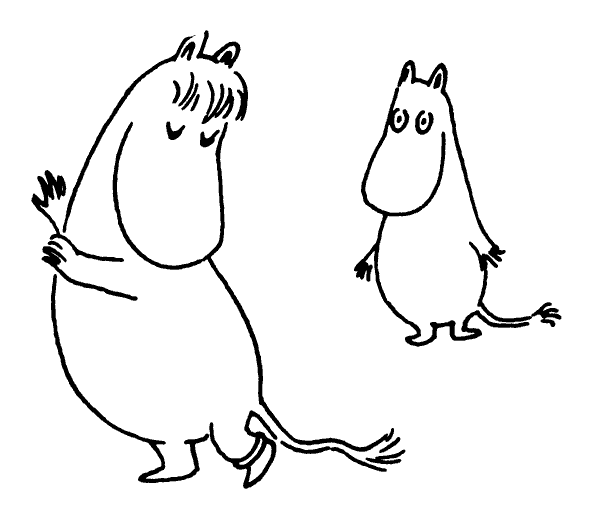
\includegraphics[width=200pt,height=176pt]{5-5.png}
\caption{}
\label{5-5}
\end{figure}

``Ŝi plendadas pri tiu ringo de pluraj tagoj,'' diris la snorko. ``Ĉiufoje kiam mi provis paroli pri la kometo ŝi parolis nur pri sia piedringo. Ĉu \emph{vi} interesiĝas pri la kometo?''

``Jes,'' respondis Snufmumriko.

``Nu, dank' al Dio,'' kontente diris la snorko. ``Do ni tuj aranĝu kunvenon. Bonvolu sidiĝi.''

Ili sidiĝis.

``Mi elektas min prezidanto kaj sekretario,'' pluis la snorko. ``Ĉu alia propono?''

Neniu havis alian proponon, kaj la snorko trifoje klakis per sia krajono al la tero.

``Ĉu estis pikformiko?'' demandis lia fratino.

``Silentu, vi ĝenas la kunvenon,'' diris la snorko. ``Kion ni scias? Jes. Ke ĝi okazos vendrede la sepan de aŭgusto je la oka kvardek du vespere. Eventuale kvar sekundojn pli malfrue.''

``La pika formiko?'' distrite diris Mumintrolo. Li kontemplis la fruntharojn de Snorkfraŭlino. Panjo ne havis fruntharojn. Li neniam antaŭe vidis fruntharojn.

``Kial neniam iu aŭskultas kion mi diras?'' malespere diris la snorko.

``Mi ne scias,'' diris Snif. ``Ĉu tiel estas de ĉiam?''

``Nun vi ĉiuj fermu la buŝon kaj aŭskultu kion diras la snorko,'' diris Snufmumriko. ``Li volas ke ni elpensu ĉu troviĝas maniero saviĝi.''

``Ni iru hejmen,'' diris Mumintrolo. ``Kaj vi akompanos nin, ĉu ne?''

``Tiun demandon ni traktu pli profunde en la sekva kunveno,'' respondis la snorko.

``Kie vi loĝas?'' demandis Snorkfraŭlino.

``Mi loĝas en belega valo kun Paĉjo kaj Panjo,'' diris Mumintrolo. ``Paĉjo mem konstruis nian domon kaj ĝi estas blua. Ĝuste antaŭ ol ekiri de hejme mi pendigis pendolilon por vi en la ĝardeno{\ldots}''

``Ej, tiam vi neniam vidis ŝin,'' vokis Snif. ``Prefere rakontu pri mia groto. Aŭskultu! Snorkfraŭlino! Ĉu vi scias ke mi havas sekreton kiu komenciĝas per K kaj finiĝas per O? Kaj ke ĝi estas treege fidema!''

``Ĉu vi ne povas zorgi pri la afero,'' petegis la snorko refoje klakante per sia krajono. ``Unue, ĉu eblas supozi ke ni atingos tiun valon antaŭ la kometo, kaj due, ĉu ni havos pli grandan ŝancon savi nin tie ol aliloke?''

``Ĝis nun ĉio prosperis,'' opiniis Snif.

``Panjo certe aranĝos tion,'' diris Mumintrolo. ``Vi devus vidi, kiel belan groton ni havas!''

``Mi havas,'' diris Snif.

``Kaj en la groto mi havas amason da perloj, kiujn mi mem kaptis,'' pluis Mumintrolo.

``Perlojn!'' ekkriis Snorkfraŭlino. ``Ĉu eblas fari piedringojn el ili?''

``\emph{Certe} eblas!'' vokis la trolo. ``Nazringojn kaj orelringojn kaj ventrozonojn kaj diademojn{\ldots}''

``Jen pli posta demando,'' diris la snorko kaj furioze batadis per sia krajono. ``Ĉu vi volas savi vin aŭ ĉu ne?''

``Nun refoje vi rompis la pinton de la krajono,'' diris lia fratino. ``Eble ni povus savi nin en tiu groto. Ĉu iu deziras vespermanĝon?''

``Kompreneble ni savu nin en la groto!'' diris Mumintrolo. ``Kiel saĝa vi estas!''

``En mia groto!'' vokis Snif. ``Ni rulos ŝtonojn antaŭ la enirejon kaj ŝtopos ĉiujn fendojn en la plafono kaj alportos amason da manĝo kaj etan lanternon. Kiel ekscite!''

``Tamen certe alia kunveno estos bezonata,'' kontraŭis la snorko. ``Pensu pri labordivido, ekzemple.''

``Kompreneble vi faru vian kunvenon,'' diris Snorkfraŭlino. ``Sed nun mi ŝatus iom da brulligno. Kaj supakvo. Kaj floroj surtable.''

``Kiu koloro?'' demandis Mumintrolo. Snorkfraŭlino rigardis sin mem kaj vidis, ke ŝi daŭre estas flava.

``Viola,'' ŝi diris, ''ŝajnas al mi ke violkoloraj floroj plej konvenus al mi. ''

Mumintrolo kuris en la arbaron. La snorko kaj Snif trenis sin for por akiri lignon kaj akvon por la supo. Snufmumriko ekbruligis sian pipon.

Li kuŝiĝis surdorse kaj rigardis supren en la ruĝan ĉielon.

``Tiu ideo pri la groto ne estis malbona,'' li diris. ``Ĉu vi timas la kometon?''

``Ne,'' diris Snorkfraŭlino. ``Se mi nur ne devas vidi ĝin kaj klopodas pensi pri io alia.''

\begin{figure}[htbp]
\centering
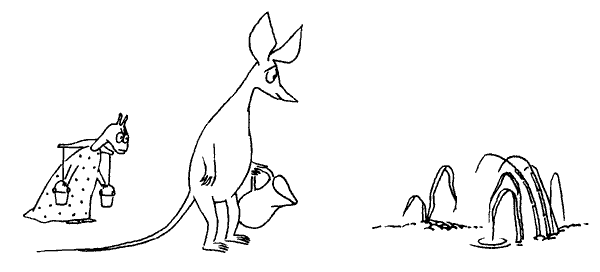
\includegraphics[width=350pt,height=158pt]{5-6.png}
\caption{}
\label{5-6}
\end{figure}

Snif trovis neniun akvon. Li flare trovis marĉon, sed tie restis nur iom da ŝlimo surfunde, kaj ĉiuj kompatindaj akvolilioj jam mortis. Fine li reiris kun pendantaj oreloj kaj diris: ``Mi pensas ke ĉiu akvo en la tuta mondo elĉerpiĝis.''

Kion ajn la fiŝoj diros pri tio. Nun restas nur fruktsuko.

``Do ni faros fruktsupon,'' diris Snorkfraŭlino. ``Jen ni solvis tiun aferon.''

``Ni certe ne solvis ĝin,'' kontraŭis ŝia frato. ``Ja devas esti ia kaŭzo ke ĉiu akvo malaperas{\ldots}''

Li sidiĝis apud la brulligno kiun li akiris. Ĉiuj ŝtipetoj estis precize same longaj, li mezuris ilin.

``Ia kaŭzo,'' malgaje ripetis la snorko.

\begin{figure}[htbp]
\centering
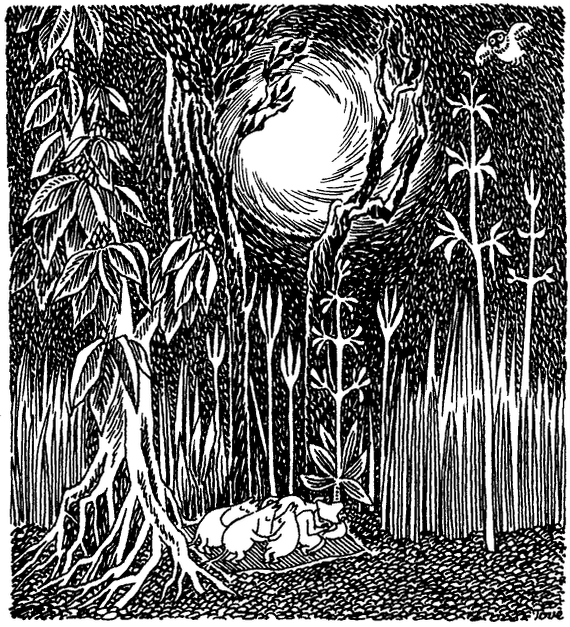
\includegraphics[width=425pt,height=467pt]{5-7.png}
\caption{}
\label{5-7}
\end{figure}

``Mi pensas ke kulpas la kometo,'' diris Snufmumriko.

Ili rigardis al la ĉielo. Krepusko komenciĝis, kaj la vespera ĉielo estis malhele ruĝa. Inter la piceoj brilis eta ruĝa fajrero kiu similis stelon. Sed ĝi ne estis stelo. Ĝi ne scintilis, ĝi ne radiis. Ĝi brulis.

Tute senmova, ĉar ĝi havis la voston malantaŭ si.

``Jen ĝi,'' diris la snorko.

La nazo de Snorkfraŭlino malrapide verdiĝis.

Mumintrolo alkuris kun bukedo kiun li klopodis fari kiel eble plej violkolora. Snorkfraŭlino rigardis ĝin.

``Mi preskaŭ pensas ke flavaj estus pli bonaj,'' ŝi diris. ``Kiel vi vidas mi verdiĝis.''

``Ĉu mi alportu novan?'' demandis Mumintrolo.

``Ne,'' ŝi diris. ``Sed pendigu ion por kaŝi tiun kometon, alie mi ne povos kuiri supon.''

Mumintrolo pendigis plejdon antaŭ la kometo. Tiam Snorkfraŭlino retrankviliĝis kaj kuiris fruktsukan supon kun manpleno da herboj en sia eta kaserolo. Poste ŝi disdonis krakpanon, ĉar la snorkoj havis nenion alian.

Post la vespermanĝo ili kuŝiĝis dense sur la dormomato el herbo, kiun Snorkfraŭlino plektis. La fajro malrapide estingiĝis kaj la nokto alvenis.

Sed super la silenta dormanta arbaro lumis la kometo, varmega kaj misaŭgura.

\chapter*[Ĉapitro 6]{Ĉapitro 6}
\addcontentsline{toc}{chapter}{Ĉapitro 6}


\begin{figure}[htbp]
\centering
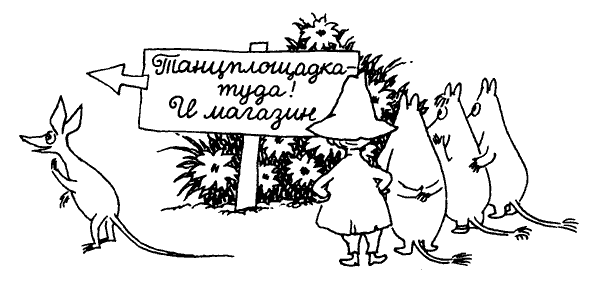
\includegraphics[width=450pt,height=214pt]{6-1.png}
\caption{}
\label{6-1}
\end{figure}

La tutan postan tagon ili marŝis tra la arbaro, rekte en la direkto al Muminvalo. Snufmumriko muzikis al ili por iom gajigi la aferon. Iam ĉirkaŭ la kvina horo ili venis al vojeto kun granda afiŝo. ``\emph{`Dancejo. Ĉi tien. Butiko'},'' diris la afiŝo.

``Ho! Mi volas danci!'' vokis Snorkfraŭlino kunfrapante la snorkmanojn.

``Ni ne havas tempon danci nun kiam la tero pereos,'' diris la snorko.

``Sed se ni entute dancu, necesas fari tion nun,'' ekkriis Snorkfraŭlino. ``Karulo! Ĝi ja pereos nur post du tagoj!''

``Eble oni povus akiri limonadon en tia butiko,'' diris Snif.

``Kaj la vojo iras preskaŭ en nia direkto,'' diris Mumintrolo.

``Oni ja povus nur \emph{rigardi} tiun dancejon,'' opiniis Snufmumriko. ``Preterpasante{\ldots}''

\begin{figure}[htbp]
\centering
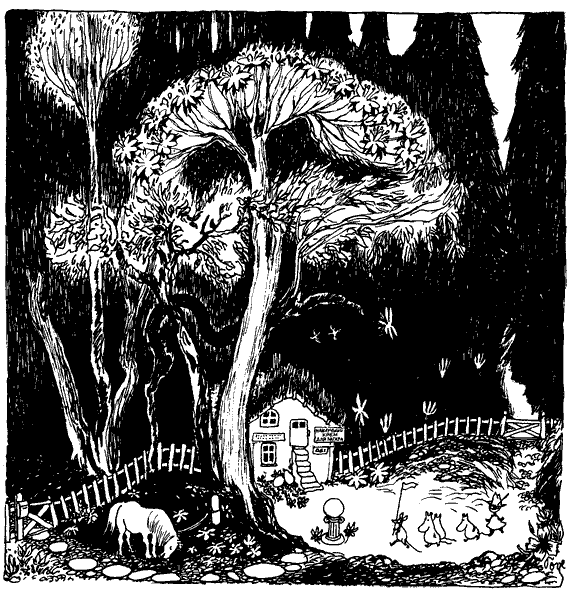
\includegraphics[width=445pt,height=462pt]{6-2.png}
\caption{}
\label{6-2}
\end{figure}

La snorko suspiris. Kaj poste ili deflankiĝis sur la vojeton. Ĝi estis vojo gaja kiu serpentis tien-reen, ĝi faris maŝojn kaj saltojn ĉiudirekten kaj foj-foje ĝi nodis sin mem pro nura petolo. Oni ne laciĝas marŝi sur tia vojo, kaj supozeble oni alvenas pli rapide per ĝi ol per vojo rekta kaj malgaja.

``Mi sentas kvazaŭ ni venus hejmen post nur momento,'' diris Mumintrolo.

``Rakontu iomete pri la valo,'' petis Snorkfraŭlino.

``Ĝi estas valo kie oni sentas sin tute sekura,'' rakontis la trolo. ``Oni ĝojas vekiĝante kaj estas agrable endormiĝi vespere.''Troviĝas arbo por grimpado, kie mi konstruos domon, kaj tute sekreta loko kiun mi montros al vi. Panjo metis konkojn ĉirkaŭ ĉiuj florbedoj, kaj sur la verando ĉiam estas sunbrilo. Tie bonodoras. Kaj ni havas propran ponton, kiun Paĉjo konstruis, kaj eblas iri per ĉarumo trans ĝin. Krome mi eltrovis la maron, peco de la maro estas nia propra{\ldots}

``Antaŭe vi nur paroladis pri kiel bele estas en ĉiuj aliaj lokoj, kie vi ne estis,'' diris Snif.

``Sed tio ja estis antaŭe,'' respondis Mumintrolo.

La vojo faris novan kurbon kaj jen estis la butiko, kaj ĝi estis eĉ tre bona butiko. Ĉirkaŭ ĝi staris ĉiaspecaj floroj en bonordaj vicoj, kaj sur fosto kuŝis arĝenta globo kiu spegulis la tutan arbaron kaj la blankan domon kun herba tegmento. Jen kaj jen pendis tabuloj kiuj rakontis, ke eblas akiri lavpulvoron kaj glicirizon kaj Unuarangan Sunoleon.

Mumintrolo supreniris laŭ la ŝtuparo kaj malfermis la pordon, kaj tiam sonorileto en la domo sonis. Ili eniris la butikon, nur Snorkfraŭlino restis ekstere por speguliĝi en la arĝenta globo. Trans la vendotablo sidis maljunulino kun brilaj musaj okuletoj kaj blanka hararo.

``Aha,'' ŝi diris. ``Tiom da infanetoj. Kaj kion vi do deziras?''

``Limonadon,'' diris Snif. ``Prefere ruĝan.''

``Ĉu troviĝas kajeroj kun linioj aŭ kvadratoj?'' demandis la snorko, ĉar li intencis noti ĉion farendan se oni kolizias kun kometo.

``Certe troviĝas,'' respondis la maljuna virino. ``Ĉu blua kajero?''

``Prefere iu alia koloro,'' diris la snorko, ĉar bluajn kajerojn uzas nur tre malgrandaj snorkoj.

``Eble mi bezonus novan pantalonon,'' diris Snufmumriko. ``Sed ĝi ne aspektu \emph{tro} nove. Mi bonfartas nur en tia kiu havas mian propran formon.''

\begin{figure}[htbp]
\centering
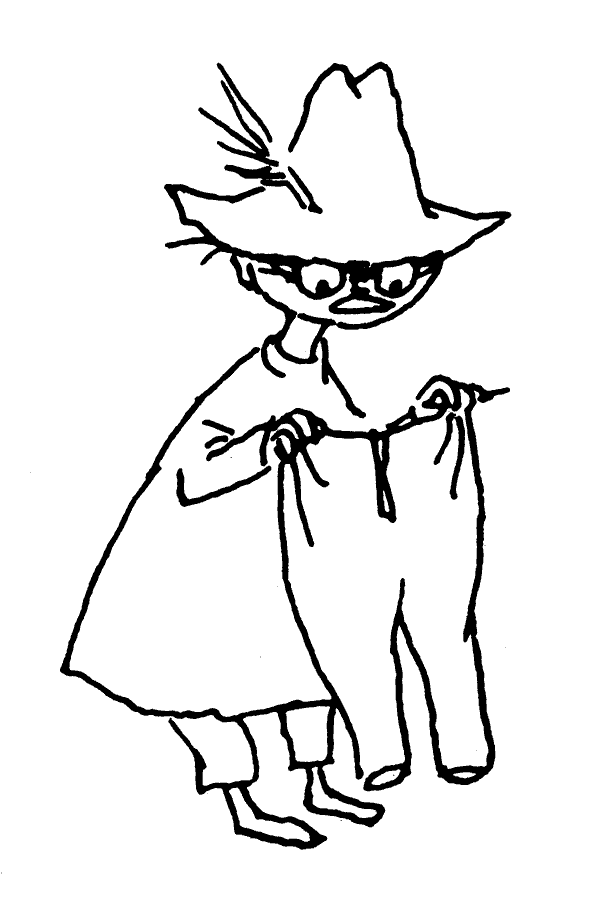
\includegraphics[width=100pt,height=153pt]{6-3.png}
\caption{}
\label{6-3}
\end{figure}

``Ĝuste tiel,'' diris la virino kaj surgrimpis ŝtupetaron por dehoki pantalonon el la plafono.

``Ĝi aspektas ege nove,'' Snufmumriko maltrankvile diris. ``Ĉu ne troviĝas pli malnova?''

``Tiu sendube estas la plej malnova pantalono kiun mi havas,'' deklaris la virino. ``Sed morgaŭ ĝi ja estos eĉ pli malnova,'' ŝi aldonis esperplene kaj rigardis Snufmumrikon super la okulvitroj.

``Nu bone,'' li diris. ``Mi povus iri trans la domangulo por provi ĝin. Sed mi demandas min ĉu ĝi havas mian formon.'' Kaj li malaperis en la ĝardenon.
\sectionbreak
La snorko notadis en sia nova kajero, kiu estis verda.

``Nu, kion deziras vi, eta trolo?'' demandis la maljunulino.

``Diademon,'' Mumintrolo serioze respondis.

``Diademon!'' diris la virino kun surpriziĝo. ``Por kio vi uzos ĝin?''

``Li donacos ĝin al Snorkfraŭlino,'' kriis Snif kiu sidis meze sur la planko trinkante ruĝan limonadon tra suĉilo.

``Li iĝis tute ridinda de kiam li renkontis ŝin.''

``Tute ne estas ridinde doni juvelojn al damo,'' diris la eta maljunulino. ``Vi estas tro malgranda por kompreni, sed efektive juvelo estas la sola ĝusta donaco por damo.''

``Ho, ĉu vere,'' diris Snif kaŝante la nazon en la limonadglaso.

La virino rigardis supren-suben laŭ ĉiuj siaj bretoj, sed tie troviĝis neniu diademo.

``Eble sub la vendotablo,'' proponis Mumintrolo.

La virino serĉis.

``Ne, ankaŭ tie ne,'' ŝi malgaje diris. ``Imagu, mi havas eĉ ne unu solan diademon. Sed eble konvenus paro da etaj snorkogantoj?''

``Mi ne vere scias,'' diris Mumintrolo kun malgaja mieno. Tiumomente la porda sonorilo sonoris kaj Snorkfraŭlino eniris la butikon.

``Bonan tagon,'' ŝi diris. ``Kian ege belan spegulon vi havas en la ĝardeno, sinjorino. De kiam mi perdis mian spegulon mi povas speguli min nur en akvoflakoj, kaj la vizaĝo iĝas iel stranga en ili.''

La virino okulumis al Mumintrolo. Ŝi prenis ion de breto kaj rapide enmanigis ĝin al li. Mumintrolo rigardis; ĝi estis eta ronda spegulo kun arĝenta rando kaj dorsflanke troviĝis ruĝa rozo farita el rubenoj. Li rigardis la maljunulinon ridante. Snorkfraŭlino nenion rimarkis.

``Vi hazarde ne havas medalojn,'' sinjorino, ŝi demandis.

``Kion?'' demandis la virino.

``Medalojn,'' diris Snorkfraŭlino. ``Belajn stelojn, kiujn sinjoroj ŝatas porti ĉirkaŭ la kolo.''

``Ho, jes ja,'' ekkriis la virino. ''Medaloj tio estas, ja. ''

Kaj ŝi rigardis supren-suben laŭ siaj bretoj kaj sub la vendotablo kaj ĉie en la butiko.

``Ĉu vi havas neniun entute,'' demandis Snorkfraŭlino kaj ekhavis larmojn en la okuloj.

La virino aspektis malfeliĉa, sed tiam ŝi ekhavis ideon kaj suriris la ŝtupetaron ĝis la plej supra breto. Ŝi eligis la skatolon kun kristarbaj ornamoj kaj singarde elprenis grandan belan stelon por la arbopinto.

\begin{figure}[htbp]
\centering
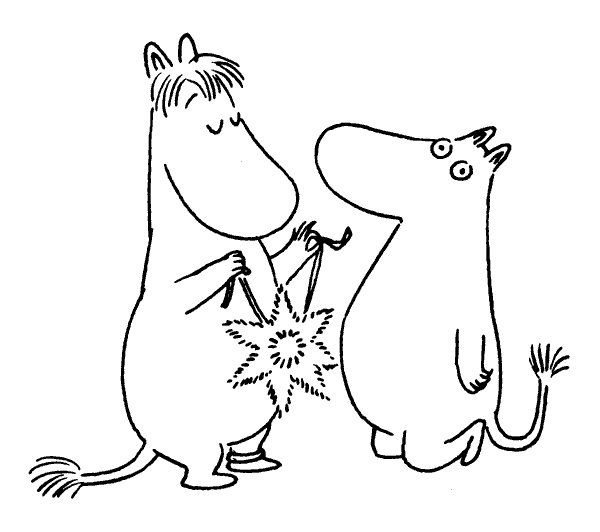
\includegraphics[width=211pt,height=186pt]{6-4.png}
\caption{}
\label{6-4}
\end{figure}

``Imagu, kia bonŝanco,'' ŝi diris. ``Jen tamen mi havas medalon!''

``Ho, kiel bela,'' flustris Snorkfraŭlino. Ŝi turnis sin al

Mumintrolo dirante: ``Ĝi estas por vi. Ĉar vi savis min de la venena arbedo.''

Mumintrolo mutiĝis kaj emociiĝis. Li genuis kaj ŝi pendigis la medalon ĉirkaŭ lian kolon. Ĝi lumis per unika brilo.

``Vi devus vidi kiel bela vi estas,'' ŝi diris.

Tiam Mumintrolo montris la spegulon, kiun li tenis kaŝita malantaŭ la dorso.

``Ĝi estas por vi,'' li diris. ``Vi povas speguli min.''

Dum ili spegulis unu la alian la porda sonorilo sonis kaj envenis Snufmumriko.

``Mi pensas ke tiu pantalono prefere iom pli malnoviĝu,'' li diris. ``Ĝi ne havas mian formon.''

``Mi bedaŭras,'' diris la virino. ``Sed novan ĉapelon vi sendube bezonus?''

Snufmumriko tiris sian malnovan ĉapelon pli suben sur la orelojn kun tima mieno.

``Koran dankon,'' li diris. ``Sed mi ĝuste rememoris kiom danĝeras akiri tro da posedaĵoj.''

La snorko senĉese sidis notante en sia kajero. Nun li stariĝis kaj diris: ``Unu grava afero pri kometoj estas ne tro longe resti elektante en butikoj. Snif! Tuj eltrinku la limonadon!''

\begin{figure}[htbp]
\centering
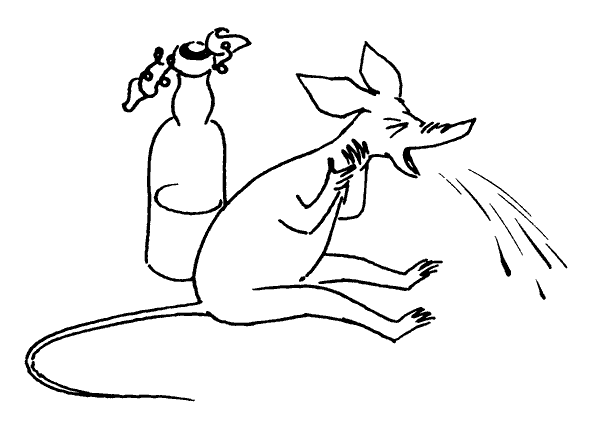
\includegraphics[width=249pt,height=176pt]{6-5.png}
\caption{}
\label{6-5}
\end{figure}

Snif verŝis en sin la tutan botelon kaj misglutis ĝin. Aŭdiĝis strangaj sonoj kaj jen li elsputis la tuton sur la maton.

``Mi vomis!'' li riproĉe ekkriis.

``Tiel li ĉiam faras,'' klarigis Mumintrolo. ``Nun ni ja baldaŭ foriros, ĉu?''

``Kiom kostas ĉio?'' demandis la snorko.

La eta maljunulino komencis kalkuli, kaj dum ŝi kalkulis, Mumintrolo ekmemoris ke li ne havas monon. Per la brovoj li demandis la aliajn kaj vidis laŭ iliaj nazoj ke ankaŭ ili estas senaj. Kurteno!

``Estos 40 penioj por la kajero kaj 34 penioj por la limonado,'' diris la virino. ``La stelo kostas 3 markojn kaj la spegulo 5 ĉar estas rubenoj dorsflanke. La tuto estos 8 markoj kaj 74 penioj.''

Neniu diris ion. Snorkfraŭlino surtabligis la speguleton kun profunda suspiro, kaj Mumintrolo komencis malnodi la ŝnuron de sia medalo. Snif rigardis la maton malsekan de limonado. Kaj la snorko demandis sin ĉu kajero pli aŭ malpli valoras post kiam oni skribis en ĝi.

La eta maljunulino rigardis ilin super la okulvitroj.

``Nu, miaj infanetoj,'' ŝi diris. ``Krome ja estas tiu malnova pantalono, kiun Snufmumriko ne deziris. Ĝi valoras precize 8 markojn.''

Unu afero forstrekas la alian, do efektive vi ŝuldas entute nenion.

``Ĉu tio povas esti ĝusta?'' scivolis Mumintrolo.

``Certe tio estas ĝusta,'' respondis la virino. ``Mi ja konservos la pantalonon.''

La snorko klopodis kalkuli enkape sed tio ne prosperis.

Do li notis ĝin ĉi tiel en sia kajero:

kajero	40 penioj

limonado (esputita)	34 penioj

medalo	3 markjoj

spegulo (kun rubenoj)	5 markoj

Sume 8 markoj kaj 74 penioj

Pantalono 8 markoj

8=8

krom 74 penioj

``Sed tio ja ĝustas,'' la snorko surprizite diris.

``Tamen restas 74 penioj,'' kontraŭis Snif. ``Ni devus havi tiujn, ĉu ne?''

``Ne estu pedanta,'' diris Snufmumriko. ``Ni diru ke tio egalas.''

Ili riverencis al la eta maljunulino. En la pordo Snorkfraŭlino demandis:

``Ĉu la dancejo estas malproksima?''

``Tute ne,'' respondis la virino. ``Iom pli antaŭe. Sed la danco komenciĝos nur je la lunleviĝo.''
\sectionbreak
Meze de arbaro Mumintrolo haltis kaj diris: ``Tiu herba tegmento ne aspektis tre forta. Eble ŝi ŝatus kuniri por kaŝiĝi en nia groto?''

``En mia groto,'' diris Snif. ``Ĉu mi iru demandi?''

``Faru tion,'' diris Snufmumriko.

Snif forkuris kaj ili sidiĝis vojrande por atendi.

``Ĉu vi scias danci tiun novan, kio-ajn-ĝi-nomiĝas?'' demandis Snorkfraŭlino.

``Ne,'' respondis Mumintrolo. ``Valso plaĉas al mi.''

``Ni ne havas tempon danci,'' diris la snorko. ``Rigardu la ĉielon.''

Ili rigardis (sed Snorkfraŭlino ne).

``Ĝi pligrandiĝis,'' diris Snufmumriko. ``Hieraŭ ĝi estis kiel formika ovo. Nun ĝi aspektas kiel oranĝo. Mi preskaŭ pensas{\ldots}''

``Sed tangon vi sendube scias,'' interrompis Snorkfraŭlino. ``Unu paŝeto flanken kaj du malantaŭen.''

``Tio ja sonas facile,'' konsentis Mumintrolo.

``Kara kokina fratino,'' diris la snorko. ``Ĉu vi neniam povas resti ĉe la afero!?''

``Ni komencis paroli pri danco,'' diris Snorkfraŭlino. ``Kaj poste vi subite daŭrigis parolante pri kometoj. Mi ankoraŭ parolas pri danco.''

Ambaŭ malrapide komencis ŝanĝi koloron. Ĝuste tiam Snif rekuris.

``Ŝi ne volas,'' li vokis. ``Ŝi savos sin en la kelo kun konfitaĵoj. Sed ŝi sendis dankojn kaj salutojn kaj po unu stangbombonon al ĉiu el ni.''

``Ĉu vi ne hazarde elpetis ilin,'' demandis Mumintrolo.

``Neniam en mia vivo!'' incitite diris Snif. ``Ŝi opiniis ke ni devus ricevi ilin ĉar ŝi ŝuldis al ni 74 peniojn. Mi diris nur, ke ŝi tute pravas.''

Do ili marŝis plu kaj la vojo marŝis kun ili. La malhela suno subiris inter piceoj kaj enlitiĝis sub la horizonto. Anstataŭe la luno leviĝis, sed ĝi estis strange palverda kaj senbrila.

La kometo lumis pli kaj pli forte. Ĝi estis preskaŭ same granda kiel la plenluno kaj lumigis la tutan arbaron per sia ruĝa, malrealeca lumo.

La dancejo situis en eta maldensejo. Ĝi estis ornamita per kronoj el lampiroj, kaj arbarrande granda akrido agordis sian violonon. La maldensejo estis plena de vizitantoj kiuj atendis ke la dancado komenciĝu. Etaj lagofantomoj kuraĝis elveni el la sekiĝintaj marĉoj kaj el la arbara lageto. Sur la dancejo estis svarmo el etaj knitoj, kaj sub la betuloj klaĉadis amaso da arbo-spiritoj (arbospirito estas eta damo kun belega hararo kiu vivas en la arbotrunko. Nokte ŝi eliras por balanciĝi en la frondaro. Ŝi kutime ne troviĝas en pinglo-arboj).

Snorkfraŭlino elprenis sian speguleton por kombi la fruntharojn kaj esplori, ĉu la floro sidas ĝuste malantaŭ ŝia orelo. Mumintrolo alĝustigis sian medalon. Ili neniam antaŭe vizitis tiel grandan balon.

\begin{figure}[htbp]
\centering
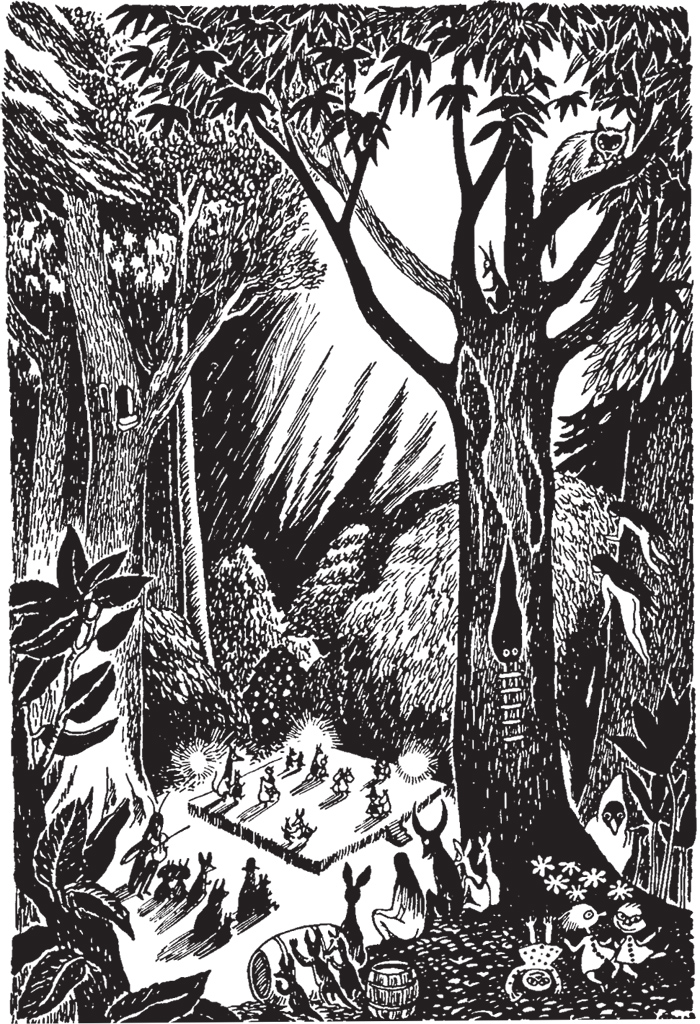
\includegraphics[width=450pt,height=658pt]{6-6.png}
\caption{}
\label{6-6}
\end{figure}

``Ĉu vi pensas ke mi ofendos la akridon, se mi iomete ludos per mia buŝharmoniko,'' flustris Snufmumriko.

``Ludu vi ambaŭ,'' diris la snorko. ``Instruu al li tiun kanton \emph{`Ĉiuj bestetoj bantigas la voston'.}''

``Ĝi konvenos,'' diris Snufmumriko. Kaj li venigis kun si la akridon malantaŭ arbedon por instrui al li la novan kanton.

Post kelka tempo aŭdiĝis etaj tonoj trans la arbedo, unu post alia, kaj jen pliaj, triloj kaj melodietoj. Knitetoj kaj arbospiritoj kaj lagofantomoj ĉesis babili kaj iris sur la herbejon por aŭskulti.

``Tio sonas bone,'' ili diris. ``Certe estas bone danci je tio.''

``Panjo,'' diris juna kniteto kaj montris al Mumintrolo. ``Tie staras generalo.''

La tuta familio venis admiri lian medalon.

``Kiel belan lanugon vi havas,'' ili diris al Snorkfraŭlino.

La arbospiritoj rajtis laŭvice speguliĝi en ŝia spegulo kun rubena rozo dorsflanke kaj ĉiu lagofantomo desegnis malsekan personan markon en la kajero de la snorko.

Sed nun aŭdiĝis la kanto `Ĉiuj bestetoj bantigas la voston' trans la arbedo, eĉ ne unu sola tono perdiĝis, kaj jen aperis Snufmumriko kaj la akrido ludante plenforte. Estiĝis granda pelmelo kaj svarmado kiam ĉiuj paroj elserĉis unu la alian. Post kelka tempo ĉiu trovis tiun, kun kiu li plej preferis danci, kaj ĉiuj turniĝis en rondo sur la dancejo.

``Sed vi ja dancas tre bone,'' diris Snorkfraŭlino. ``Kiu danco estas tio?''

\begin{figure}[htbp]
\centering
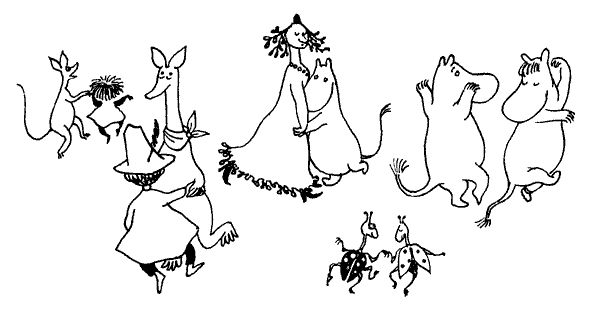
\includegraphics[width=350pt,height=182pt]{6-7.png}
\caption{}
\label{6-7}
\end{figure}

``Mia propra,'' respondis Mumintrolo. ``Mi ĵus eltrovis ĝin!''

La snorko elektis lagvirineton kun perkoherboj en la haroj kaj trovis iom malfacile sekvi la takton. Snif turniĝis kun la plej malgranda kniteto kaj sentis sin tre granda. Estis klare ke la knito admiris lin.

La kuloj dancis sialoke kaj el ĉiuj anguloj de la arbaro novaj gastoj alplandis, alrampis kaj alsaltis por rigardi. Neniu sola pensis pri la kometo kiu sola kaj arda flugis antaŭen tra la nigra nokta spaco.

Proksimume je noktomezo oni alrulis grandan barelon da pomvino, kaj ĉiu ricevis etan tason el betulŝelo el kiu trinki. La lampiroj kolektiĝis en bulon meze de la dancejo kaj ĉirkaŭe sidis ĉiuj aliaj manĝante buterpanojn kaj trinkante vinon.

``Nun ni rakontu historiojn,'' diris Snif. ``Ĉu vi ne scias rakonton, eta knito?''

``Neee,'' diris la knito kaj terure embarasiĝis. ``Eble unu{\ldots}''

``Nu, do rakontu ĝin,'' diris Snif.

``Estis iam arbara rato nomita Pimp,'' murmuris la knito kaj timide rigardis inter la manoj.

``Nu, kaj kio poste?'' diris Snif kuraĝige.

``La rakonto finiĝis nun,'' flustris la knito kaj subenrampis por kaŝiĝi en la muskoj. Ĉiuj ridis plenforte, kaj la lagofantomoj batadis tamburon per siaj vostoj.

\begin{figure}[htbp]
\centering
\includegraphics[width=100pt,height=116pt]{6-8.png}
\caption{}
\label{6-8}
\end{figure}

``Ludu ion al kio eblas fajfi!'' vokis Mumintrolo.

``Do ni ludu la Paŝto-paŝanto-kanton,'' diris Snufmumriko.

``Sed ĝi estas tiel malĝojiga,'' kontraŭis Snorkfraŭlino.

``Tamen ludu ĝin,'' diris Mumintrolo. ``Ĝi estas bona fajfokanto.''

La mumriko ludis kaj la trolo fajfis kaj ĉiuj aliaj kunkantis en la rekantaĵo:

\emph{Vi paŝta paŝanto}

\emph{jen fajfu kaj kantu}

\emph{en nokta malvarm'.}

\emph{Vi lacas ĉi fojon}

\emph{kaj perdis la vojon}

\emph{al hejma la ĉarm'.}

Snorkfraŭlino suspiris.

``Nun mi iĝis melankolia,'' ŝi diris. ``Tio ja estas precize kiel pri ni. Ni estas lacaj kaj perdis la vojon hejmen!''

``Vi estas laca ĉar vi tro multe dancis,'' diris la snorko kaj malplenigis sian tason.

``Kompreneble ni trovos la vojon hejmen,'' vokis Mumintrolo. ``Ne estu melankolia! Ni hejmenvenos kaj Panjo havos pretan vespermanĝon kaj diros `imagu ke prosperis al vi' kaj ni diros `vi ne scias kion ni trapasis!'''

``Kaj mi ricevos piedringon el perloj,'' flustris Snorkfraŭlino. ``El unu perlo ni faros kravatpinglon por vi.''

``Jes,'' diris Mumintrolo. ``Kvankam ja sufiĉe malofte mi portas kravaton.''

``Unu perlon mi pendigos ĉirkaŭ la kolon de mia sekreto,'' diris Snif. ``Mi havas sekreton, kiu komenciĝas per K kaj finiĝas per O kaj kiu akompanas min ĉie! Ĝi sopiris al mi dum la tuta tempo nun kiam mi forestis{\ldots}''

``Ĉu ĝi eble finiĝas per to?'' demandis la snorko.

``Mi ne diras!'' vokis Snif. ``Kaj vi ne rajtas diveni!''

Nun Snufmumriko ludis unu kanton post alia, dormemigajn krepuskajn kantojn kaj ekirajn kantojn. Unu post la alia knitetoj kaj lagofantomoj komencis retiriĝi en la arbaron. La arbospiritoj malaperis kaj Snorkfraŭlino endormiĝis kun sia spegulo enmane.

Fine la kantoj silentiĝis kaj sur la herbejo estis tute kviete. La lampiroj estingiĝis, kaj tre, tre malrapide alproksimiĝis la mateno.

\chapter*[Ĉapitro 7]{Ĉapitro 7}
\addcontentsline{toc}{chapter}{Ĉapitro 7}


La kvinan de aŭgusto birdoj ne plu kantis. La suno lumis tiel malforte ke ĝi apenaŭ estis videbla. Sed super la arbaro la kometo staris granda kiel rado de veturilo, kaj ĉirkaŭ ĝi estis ringo el fajro.

Snufmumriko ne emis muziki. Li paŝis solece cerbumante. Ankaŭ la aliaj estis silentaj. Nur Snif de temp' al tempo ĝemetis kaj plendis pri kapdoloro. Estis terure varmege.

Tiam la arbaro malfermiĝis en dezertan pejzaĝon el longaj sablodunoj. Senfinaj molaj montetoj el sablo kaj jen kaj jen tufoj el mara aveno. Mumintrolo haltis flarante en la aero.

``Mi ne sentas marodoron,'' li diris. ``Malbonodoras{\ldots}''

``Sendube estas dezerto,'' diris Snif malgaje. ``Dezerto kie niaj ostoj blankiĝos kaj eĉ neniam estos trovitaj. Mi havas kapdoloron!''

Estis peze paŝi sur la sablo. Ili plumarŝis, super unu altaĵo kaj suben laŭ alia.

``Jen rigardu,'' diris la snorko. ``La hatifnatoj migras.''

Fore sur la dunoj moviĝis longa procesio el hatifnatoj. Ili rigide okulfiksis la horizonton kaj maltrankvile flirtigis la manojn.

\begin{figure}[htbp]
\centering
\includegraphics[width=449pt,height=223pt]{7-1.png}
\caption{}
\label{7-1}
\end{figure}

``Ili marŝas orienten,'' diris la snorko. ``Eble plej sekure estus sekvi ilin. Ili sentas, vi scias.''

``Sed ni loĝas okcidente,'' diris Mumintrolo. ``Paĉjo kaj Panjo loĝas okcidente.''

Kaj li pluiris laŭ rekta linio kontraŭ Muminvalon.

``Nun mi krome soifas,'' plendis Snif.

Sed neniu respondis.

La sablodunoj malaltiĝis. La tero estis kovrita de maraj fukoj kiuj brilis ruĝe en la kometa lumo. Troviĝis silikoj kaj konkoj. Troviĝis pecoj da betulŝelo kaj ligno kaj korko, troviĝis ĉio kio devas troviĝi sur mara strando. Sed la maro ne plu troviĝis.

Ili staris unu apud la alia nur gapante. Kie devus esti la maro kun siaj molaj bluaj ondoj kaj balanciĝantaj mevoj nun troviĝis nur malfermita abismo. Vaporis el ĝi, io bolis tie sube, kaj odoris strange kaj akre.

Sub ili la strando apikis suben en verdajn, ŝlimajn fendegojn.

\begin{figure}[htbp]
\centering
\includegraphics[width=448pt,height=371pt]{7-2.png}
\caption{}
\label{7-2}
\end{figure}

``La maro estas for,'' diris Snorkfraŭlino duonvoĉe. ``Kial la maro malaperis?!''

``Mi ne scias,'' murmuris Mumintrolo.

``Bone do, ke ni ne estas fiŝoj,'' diris Snif, klopodante esti brava.

Sed Snufmumriko sidiĝis kun la kapo en la manoj kaj vokis: ``La bela maro! Tute for! Plu neniu velado, neniu naĝado, neniuj grandaj ezokoj! Neniuj ŝtormegoj, neniu travidebla glacio! Neniam plu la luno povos speguli sin! Kaj la strando ne plu estas strando, ĝi estas nenio ajn!''

Mumintrolo sidiĝis apud lin kaj diris:

``Ĝi revenos. Ĉio revenos post kiam la kometo foriros. Ĉu vi ne kredas ke jes?''

Sed Snufmumriko ne respondis.

``Kiel ni trairu?'' subite demandis la snorko. ``En du tagoj ni ne havas tempon ĉirkaŭiri tiun truon.''

Neniu ion diris.

``Ni devas kunveni,'' pluis la snorko. ``Mi proponas min kiel prezidanton kaj sekretarion. Ĉu vi havas proponojn?''

``Flugi,'' diris Snif.

``Paŝi,'' murmuris Mumintrolo.

``Ne estu stultaj,'' diris la snorko. ``Ni ne havas tempon esti stultaj. Viaj proponoj estas unuanime malakceptataj. Proponu ion alian.''

``Proponu mem!'' kriis Mumintrolo kolere. ``Troviĝas neniu maniero! Skribu en via aĉa kajero ke ni ĉiuj iĝos kaĉo kiam la kometo venos ĉar eĉ Snufmumriko ne kredas ke ni elturniĝos!''

Iĝis tute silente.

Tiam Snufmumriko stariĝis kaj diris: ``Ni trairos per stilzoj. Por tio la tempo sendube sufiĉos.''

``Jes ja!'' vokis Mumintrolo. ``Jen bona ideo! Stilzoj, kompreneble! Rapidu! Ni devas trovi stilzojn, ni savos nin, ni venos hejmen!''

Ĉiuj diskuris por serĉi.

Nenie eblas trovi tiel multe kiel sur mara strando. Mumintrolo trovis okcidentan balizon disrompitan. Snorkfraŭlino trovis tenilon de balailo kaj remilon. Snufmumriko trovis fiŝvergon kaj flagstangon. Snif trovis lupolan apogilon kaj difektitan ŝtupetaron. Sed la snorko iris la tutan vojon reen ĝis la arbaro kaj akiris du mallarĝajn trunkojn de piceoj precize same longaj.

Poste ili ĉiuj renkontiĝis denove kaj klopodis lerni paŝi per stilzoj.

Snufmumriko stabile iris tien-reen per siaj stilzoj montrante al la aliaj kiel oni faru.

\begin{figure}[htbp]
\centering
\includegraphics[width=430pt,height=238pt]{7-3.png}
\caption{}
\label{7-3}
\end{figure}

``Pli longajn paŝojn!'' li vokis. ``Estu tute trankvilaj. Ne pensu. Sentu! Ne rigardu suben, ĉar tiam vi perdos la ekvilibron.''

``Mi havas kapturnon! Mi vomos!'' kriis Snif.

``Aŭskultu, Snif,'' diris Snufmumriko. ``Estas tre eble, ke troviĝas \emph{perditaj trezoroj} sur la mara fundo.''

Kaj Snif tuj ĉesis malbonfarti.

``Rigardu min,'' vokis Snorkfraŭlino. ``Mi kapablas! Mi kapablas! Mi tute ne pensas, mi nur sentas!''

``Tion ni scias,'' diris ŝia frato.

Post unu horo diris Snufmumriko: ``Nun ŝajnas al mi ke vi ĉiuj kapablas. Estas tempo ekiri.''

``Ankoraŭ ne! Mi sendube devas iom pli ekzerci min,'' petis Snif kaj ĵetis rapidan rigardon suben en la maran fundon.

``Ni ne havas tempon,'' diris la mumriko. ``Nun memoru eviti ŝlimon kaj fendojn. Sekvu min.''

Unu post la alia, kun la stilzoj sub la brakoj, ili grimpis suben en la ruĝa krepusko. Ili perdis piedapogon kaj glitis sur la marherboj kaj apenaŭ povis vidi unu la alian pro akvovaporo.

``Vi memoras ke ĉi tio okazas je via risko, ĉu ne?'' demandis Snif.

``Certe,'' respondis Mumintrolo. ``Mi scias. Vi povas esti tute trankvila.''

Nun la morta mara fundo etendiĝis antaŭ ili. Ĝi aspektis vere mizera.

Ĉiuj belaj kronoj el fuko, kiuj iam balanciĝadis en travidebla akvo, kuŝis plataj kaj nigraj, kaj fiŝoj senpove baraktis en la malmultaj flakoj restantaj. Terure malbone odoris. Ĉie meduzoj kaj fiŝetoj kuŝis spirkaptante, kaj Snorkfraŭlino kuris tien-reen por porti ilin ĝis la akvotruoj.

``Tiel do, tiel do,'' ŝi diris. ``Nun vi tuj fartos bone denove{\ldots}''

``Mi ege bedaŭras,'' diris Mumintrolo. ``Sed mi pensas ke ni ne havos tempon savi ĉiujn.''

``Tamen kelkajn,'' diris Snorkfraŭlino suspirante. Ŝi suriris siajn stilzojn kaj sekvis la ceterajn. Ĉi-malsupre la kometo impresis multe pli granda, kaj ĝi ŝajnis flirti kaj flagri tra la akvovaporo. Kvazaŭ long-kruraj insektetoj ili marŝis pli kaj pli fore suben en la profundaĵojn de la maro.

\begin{figure}[htbp]
\centering
\includegraphics[width=449pt,height=658pt]{7-4.png}
\caption{}
\label{7-4}
\end{figure}

Jen kaj jen el la sablo altiĝis enormaj malhelaj montoj, kies pintoj iam estis insuletoj kaj ŝeroj kie ekskursaj boatoj albordiĝis kaj knitetoj plaŭde banis sin.

``Mi neniam plu kuraĝos naĝi en profunda akvo,'' diris Snif tremante. ``Nur imagi, ke ĉio ĉi kuŝas sub la ventro!''

Li rigardis suben en fendegon kie ankoraŭ akvo restis kaj sekreta vivo svarmis.

``Tamen ĝi estas bela. Terura kaj bela,'' diris Snufmumriko. ``Kaj scii, ke neniu iam estis ĉi tie antaŭ ni{\ldots}''

``Jen ĝi estas!'' subite kriis Snif. ``La trezorkesto! Vi diris ke ĉi tie troviĝas perditaj trezoroj{\ldots}''

Li lasis la stilzojn kaj komencis furioze elfosi la keston el la sablo.

``Helpu min!'' li kriis. ``Ĝi estas ŝlosita{\ldots} Ĝi fiksiĝis{\ldots}''

``Ni ne povos kunporti ĝin, ĝi estas tro granda,'' diris la snorko. ``Snif, mi petas, rapidu! Vi trovos multe pli belajn aferojn antaŭ ol ni alvenos.'' Kaj la besteto Snif plupaŝis kun la nazo ĉifita pro malespero.

La rokoj iĝis pli altaj kaj sovaĝaj, kaj la grundo estis plena de fendegoj. La stilzoj senĉese fiksiĝis en la fendoj, kaj ili iris pli kaj pli malrapide. Jen kaj jen iu el ili falis surkapen. Ili jam ĉesis interparoli kaj nur marŝis, marŝadis. Kaj subite sinkinta ŝipo kuŝis antaŭ ili. La kompatinda ŝipo aspektis ege melankolia. La masto estis disrompita kaj la frakasitaj flankoj plenaj de mituloj kaj marherboj. La rigon forportis maraj fluoj. Sed la prua figuro restis. Ĝi gapis rekte preter ili kaj malĝoje ridetis en soleco.

``Ĉu vi pensas ke ili saviĝis?'' flustris Snorkfraŭlino.

``Kompreneble,'' respondis Mumintrolo. ``Ili ja havis savboatojn. Venu, ni foriru. Ĝi aspektas vere tro malĝojiga.''

``Atendu iomete,'' vokis Snif kaj saltis suben de la stilzoj. ``Mi vidas ion glimantan! Ion el oro!'' Li enrampis sub la vrako kaj komencis fosi inter la marherboj.

\begin{figure}[htbp]
\centering
\includegraphics[width=150pt,height=159pt]{7-5.png}
\caption{}
\label{7-5}
\end{figure}

``Ponardo!'' li kriis. ``Ĝi estas el oro kaj havas juvelojn sur la tenilo!''

Snorkfraŭlino klinis sin antaŭen por rigardi kaj perdis la ekvilibron.

Ŝi baskulis antaŭen sur la stilzoj, poste ŝi baskulis dorsen, ŝi kriis diskante kaj jen ŝi flugis arke en la nigran internon de la vrako.

Mumintrolo alkuris por savi ŝin.

Li grimpis supren laŭ la rusta ankroĉeno, glitis sur felo el marherboj sur la ferdeko kaj rigardis suben en la mallumon de la holdo.

``Kie vi estas?!'' li kriis.

``Jen!'' pepis Snorkfraŭlino.

``Ĉu vi vundiĝis?'' demandis la trolo.

``Ne, sed mi timas,'' ŝi diris.

Mumintrolo saltis en la holdon. Akvo atingis ĝis lia ventro, kaj odoris mucide kaj malagrable.

``Snif kaj liaj ĉiamaj juveloj,'' li diris.

``Tamen mi komprenas lin,'' kontraŭis Snorkfraŭlino. ``Mi amas juvelojn kaj oron kaj perlojn kaj diamantojn! Eble troviĝas kelkaj ĉi tie! Ĉu ni{\ldots}?''

``Estas tro mallume,'' diris Mumintrolo. ``Kaj eble troviĝas danĝero ĉi tie.''

``Jes,'' obeeme diris Snorkfraŭlino. ``Do levu min, mi petas.''

Kaj Mumintrolo levis ŝin sur la randon de la holda truo.

``Kiel prosperas al vi?'' vokis Snufmumriko.

``Mi refoje estas savita,'' gaje respondis Snorkfraŭlino kaj elprenis sian speguleton por esplori ĉu ĝi frakasiĝis. Sed dank' al Dio, la vitro estis en ordo kaj ĉiuj rozaj rubenoj restis dorsflanke. En la spegulo Snorkfraŭlino vidis sian propran malsekan frunthararon, ŝi vidis la nigran truon, ŝi vidis la okulojn de Mumintrolo tie sube kaj malantaŭ li, plej fore en la mallumo ŝi vidis ion alian --- ion kio moviĝis. Kio malrapide rampis pli kaj pli proksimen al Mumintrolo{\ldots}

``Atentu!'' ŝi kriis. ``Estas io malantaŭ vi!''

Mumintrolo turnis sin.

Kaj jen venis la sepio. La plej danĝera monstro de la maro, giganta sepio, malrapide alglitis kontraŭ li el la mallumo.

Mumintrolo klopodis grimpi, sed la tabuloj estis tro glitaj. Fojon post fojo li glitis malantaŭen kaj plaŭde refalis en la akvon. Supre Snorkfraŭlino sidis kriante, ankoraŭ kun la spegulo enmane.

Kaj la sepio alproksimiĝis.

\begin{figure}[htbp]
\centering
\includegraphics[width=449pt,height=364pt]{7-6.png}
\caption{}
\label{7-6}
\end{figure}

Subite ĝi haltis palpebrumante. La spegulo kaptis la ardan diskon de la kometo per sia vitro kaj ĵetis grandan blindigan rebrilon rekte en la vizaĝon de la sepio. Ĝi ektimis. Dum sia tuta vivo ĝi vivadis en mallumo plej sube en la plej profunda maro. Nun la mallumo estis for. La maro estis for. Kaj plej terure; ekhavi abomenan, ruĝan lumon rekte en la okulojn. La sepio suspiris kaj ĵetis ĉiujn siajn brakojn ĉirkaŭ la kapon plej interne de la holdo.

``Snorkfraŭlino, vi savis mian vivon,'' diris Mumintrolo. ``Kaj en kia inteligenta maniero!''

``Tio okazis pro hazardo,'' ŝi respondis. ``Sed mi dezirus savi vin de sepio unufoje ĉiutage!''

``Nu, bone,'' diris Mumintrolo. ``Nun vi eble tamen deziras tro multe. Venu. Mi volas foriri de ĉi tie.''

Dum la tuta tago ili marŝis tra la soleca mara pejzaĝo, pli kaj pli profunde suben. Jen troviĝis enormaj marfundaj konkoj, kiuj tute ne similis tiujn, kiujn oni povas kolekti surstrande. Ili estis ornamitaj per dornoj kaj turboj kaj havis intensajn belajn kolorojn.

\begin{figure}[htbp]
\centering
\includegraphics[width=324pt,height=206pt]{7-7.png}
\caption{}
\label{7-7}
\end{figure}

``Eblus loĝi en ili,'' diris Snorkfraŭlino. ``Ĉu vi aŭdas ilin susuri? Ĉu iu sidas flustrante en ili?''

``Tio estas la maro,'' diris Snufmumriko. ``La konko memoras la maron.'' Li ekemis muziki kaj elpoŝigis la buŝharmonikon. Sed eĉ ne unu sono elvenis el ĝi, la akvovaporo forpelis ĉiujn tonojn.

``Jen aĉa afero,'' diris Snufmumriko afliktite.

``Paĉjo sendube riparos ĝin kiam ni venos hejmen,'' diris Mumintrolo. ``Li povas ripari ĉion ajn, se li nur iam komencas.''

``Nun ni estas proksime al la plej granda mara profundo,'' diris Snufmumriko. ``Paŝu singarde{\ldots}''

Jen ne plu troviĝis marherboj. La fundo de la maro krute deklivis antaŭ ili, kovrita de griza ŝlimo. Estis absolute silente kaj tre solene. Kaj jen, subite, ne plu troviĝis fundo. Ĝi malaperis en abismo el ombroj kaj akvovaporo.

\begin{figure}[htbp]
\centering
\includegraphics[width=350pt,height=413pt]{7-8.png}
\caption{}
\label{7-8}
\end{figure}

Neniu iris ĝis la rando por rigardi. Ili silente preteriris. Nur Snorkfraŭlino turnis sin kaj iomete suspiris, ĉar ĝuste ĉe la krutaĵo kuŝis la plej granda kaj bela konko de la maro. Ĝi estis tre blanka kaj lumis tra la krepusko. La maro kantis en ĝi.

``Ne zorgu pri ĝi,'' diris Mumintrolo. ``Ĉi tie estas danĝere. Tie sube troviĝas monstroj kiujn neniu iam vidis. Ili vivas tie sube en la ŝlimo{\ldots}''

Nun vesperiĝis. Ili tenis sin kiel eble plej proksime unu al la alia kaj aŭskultis la malrealecan silenton. Ĉio estis mola kaj malseka kaj strange silenta. Mankis ĉiuj amikaj sonetoj kiuj alvenas vespere sur la tero, de folioj movataj de la nokta vento, de birda pepo, de paŝoj kiuj rapidas hejmen. Ne eblis fari fajron, kaj ili timis dormi inter ĉiuj nekonataj danĝeroj, kiuj ĉi-sube povus insidi. Fine ili grimpis sur altan rokon, kie ŝajnis iom pli sekure, kaj manĝis tion kio restis el la krakpano de la snorkoj.

Mumintrolo prenis la unuan vaĉon kaj decidis preni ankaŭ tiun de Snorkfraŭlino. Dum la ceteraj kuŝiĝis dense unu ĉe la alia kaj endormiĝis, li sidis gapante al la morta mara fundo. Ĝi estis ruĝa pro la kometa lumo, sed ĉiuj ombroj estis velure nigraj.

Mumintrolo rigardis la malgajan pejzaĝon kaj pensis pri tio, kiel la tero devas timi vidante la brilan fajroglobon alproksimiĝi. Li pensis pri tio, kiom li ege amis ĉion, la arbaron kaj maron, la pluvon kaj venton, la sunbrilon kaj herbojn kaj muskojn, kaj kiel maleblus al li vivi sen ĉio ĉi.

Sed poste li pensis: `Panjo sendube scias kiel savi ĉion.'

\begin{figure}[htbp]
\centering
\includegraphics[width=200pt,height=138pt]{7-9.png}
\caption{}
\label{7-9}
\end{figure}

\chapter*[Ĉapitro 8]{Ĉapitro 8}
\addcontentsline{toc}{chapter}{Ĉapitro 8}


Snif vekiĝis kaj diris: ``Morgaŭ ĝi venos.''

Ĉiuj rigardis la kometon (eĉ Snorkfraŭlino, sed tra la fruntharoj). Ĝi timige grandiĝis. Ĉirkaŭ si ĝi havis kronon el tremantaj flamoj. La akvovaporo malaperis, kaj eblis vidi foren super la mara fundo.

``Bonan matenon!'' diris Snufmumriko kaj tiris la ĉapelon suben sur la orelojn. ``Nun ni pluiru!''

Je matenmanĝa horo ili renkontis skruton kiu iris bicikle kun sia ido en sako surdorse. Sur la pakaĵtenilo ĝi havis sian valizon, kaj amaso da pakoj kaj skatoloj pendis sur la stirilo.

\begin{figure}[htbp]
\centering
\includegraphics[width=364pt,height=180pt]{8-1.png}
\caption{}
\label{8-1}
\end{figure}

La skruto estis tute ruĝvizaĝa kaj gapis al ili sen saluti.

``Saluton,'' vokis Mumintrolo. ``Ĉu vi ne rekonas min? Ĉu vi transloĝiĝos?''

La skruto elseliĝis de la biciklo kaj rapide diris:

``Ĉiuj en Muminvalo jam foriris. Ĉu vi pensas ke ni intencas resti por atendi la kometon?!''

``Kiu diris ke la kometo falos en Muminvalon?'' demandis la snorko.

``La moskorato,'' respondis la skruto.

``Nu, tamen Paĉjo kaj Panjo,'' vokis Mumintrolo. ``Ili ja restas! Ili atendas min!''

``Jesjesjes,'' diris senpacience la skruto. ``Ili sidas en la verando. Sed tio ne koncernas min! Cetere vi ne havas tempon atingi tien{\ldots}''

Kaj la skruto plu biciklis kun hirtaj haroj.

Ili restis kelkan tempon rigardante post li.

``Valizo!'' diris Snufmumriko. ``Pakoj kaj skatoloj! En ĉi tiu varmego. Venu, ni pluiru.''

Iom pli fore ili vidis plurcent hatifnatojn survoje orienten. Sur la tuta fundo de la maro svarmis fuĝantoj. Etuloj kaj knitoj ĉiuspecaj, musaj familioj kaj muskaj troloj kaj arbaranoj, kaj ĉiuj survojis for de Muminvalo. La plej multaj venis piede, kelkaj el la pli ekscititaj kuris, sed la plej grandaj familioj akiris ĉarojn aŭ eĉ veturilon, kaj iuj kunportis sian tutan domon. Ĉiuj ĵetis timajn rigardojn alĉielen, kaj preskaŭ neniu havis tempon diri pli ol `saluton'.

``Kiel strange,'' diris malgaje Mumintrolo. ``Mi konas tiel multajn el ili, kaj ni jam delonge ne renkontis unu la alian. Kaj ĝuste nun troviĝas tiom por priparoli!''

``Ili timas,'' diris Snufmumriko.

``Ej,'' diris Mumintrolo. ``Hejme nenio povas esti danĝera!''

\begin{figure}[htbp]
\centering
\includegraphics[width=417pt,height=138pt]{8-2.png}
\caption{}
\label{8-2}
\end{figure}

``Kredeble ni estas ege kuraĝaj!'' vokis Snif gestante per sia ponardo tiel ke la juveloj glimis.

``Mi pensas, ke ni ne estas tre kuraĝaj,'' cerbumis Mumintrolo. ``La afero estas nur, ke ni jam kutimiĝis al tiu kometo. Preskaŭ interkonatiĝis kun ĝi. Ni estis la unuaj kiuj sciis ion pri ĝi, kaj ni vidis ĝin kreski kaj grandiĝi. Imagu, kiel sola ĝi devas esti{\ldots}''

``Jes,'' diris Snufmumriko. ``Imagu, kiel sola oni estus, se oni timigus ĉiujn.''

Snorkfraŭlino enŝovis sian manon en tiun de Mumintrolo.

``Ĉiuokaze,'' ŝi diris. ``Dum vi ne timos, ankaŭ mi promesas ne timi.''
\sectionbreak
Kaj finfine ili atingis la alian bordon. Ili saltis suben de la stilzoj kaj rulis sin sur la sablo, ili kuris en la arbaron, ili kriis kaj ridis kaj brakumis unu la alian.

``Ni preskaŭ venis hejmen!'' vokis Mumintrolo. ``Rapidu! Rapidu! Paĉjo kaj Panjo sidas atendante en la verando!''

Sed la vojo hejmen estis multe pli longa ol ili pensis.

En la arbaro ili renkontis hemulon kiu kverelis al si mem kun poŝtmarkalbumo enmane.

``Bruo kaj kurado,'' diris la hemulo. ``Bruo kaj kriado kaj eĉ ne unu sola povas klarigi, pri kio temas!''

``Saluton,'' diris Mumintrolo. ``Ĉu vi estas parenco de la hemulo kiu ŝatis noktan papilion?''

``Li estas mia kuzo ĉe la patra flanko,'' respondis la hemulo kun malbone kaŝita antipatio. ``Jen granda azeno. Ni ne plu estas parencoj, mi finis la rilaton.''

``Kial?'' demandis Snif.

``Li estis tro unuflanka,'' diris la hemulo. ``Nenio krom insektoj kaj insektoj kaj insektoj. La tero povus fendiĝi sub li, kaj li ne zorgus pri tio.''

``Sed ĝuste tion ĝi faros,'' klarigis la snorko. ``Pli precize morgaŭ je la oka kvardek du.''

``Kion?'' diris la hemulo. ``Do, terura bruado. Mi ordigis miajn poŝtmarkojn dum tuta semajno kaj esploris ĉiun akvomarkon, kaj kio okazas? Oni foriras kun la pordo. Oni forŝiras la seĝon. Oni fermas la tutan domon! Kaj jen mi sidas kun miaj poŝtmarkoj en plena pelmelo kaj neniu sola povas klarigi pri kio temas!''

\begin{figure}[htbp]
\centering
\includegraphics[width=301pt,height=160pt]{8-3.png}
\caption{}
\label{8-3}
\end{figure}

``Kara hemulo,'' diris Snufmumriko tre malrapide kaj klare. ``Temas pri kometo kiu morgaŭ kolizios kun la tero.''

``Kolizios,'' ripetis la hemulo. ``Ĉu tio iel rilatas al kolektado?''

``Ne, tute ne,'' diris Snufmumriko. ``Tio rilatas al sovaĝa stelo kun vosto. Kaj kiam ĝi alvenos ĉi tien, restos malmulte el viaj poŝtmarkoj.''

``Gardu min,'' diris la hemulo kaj kunigis siajn jupojn (ĉar hemuloj estas vestitaj per jupo, neniu scias kial. Eble ili neniam ekhavis la ideon surmeti pantalonon).

``Kion mi faru,'' la hemulo do pluis.

``Vi venu kun ni,'' diris Snorkfraŭlino. ``Vi povos kaŝi kaj vin mem kaj viajn poŝtmarkojn en nia bela groto.''

``Mia bela groto,'' diris Snif.
\sectionbreak
Tiel do okazis, ke la hemulo kuniris en la marŝo kontraŭ Muminvalo. Li estis tre ĝena akompananto, sed tio estis neevitebla. Unufoje ili devis reiri plurajn kilometrojn por serĉi mispresaĵon kiun li perdis, kaj dufoje li ekkverelis kun la snorko pri io kion neniu el ili bone sciis (ili asertis ke tio estis diskuto, sed ĝi sonis kiel kverelo).

Snif iris unuope kaj estis nekutime silenta. Li pensis pri la katido. Ĉu la patrino de Mumintrolo memoris elmeti lakton al ĝi? Imagu, se la katido ne komprenos ke ĝi ŝatu Snif'on, kaj anstataŭe ekŝatos la patrinon? Ĉu ĝi frotos sin al li aŭ nur foriros kun la vosto ĉielen?

Neniam eblas esti certa pri sia kato. Plej sekure estas nur subkomprenigi, ke oni havas ion kio ege multe amas onin. Snif tre fieris, ke dum la tuta vojaĝo li ne diris eĉ unu vorton pri katido.

``Aŭdu,'' subite diris Snufmumriko kaj elbuŝigis la pipon. ``Komencas blovi{\ldots}''

Ili haltis por aŭskulti. Fore en la arbaro aŭdiĝis siblado kiu rapide laŭtiĝis en malfortan ululon. Sed la arboj ne moviĝis.

``Rigardu!'' kriis la snorko.

\begin{figure}[htbp]
\centering
\includegraphics[width=400pt,height=58pt]{8-4.png}
\caption{}
\label{8-4}
\end{figure}

Alte super la arbopintoj granda nubo alflugis, nubo kiu altiĝis kaj malaltiĝis kaj ombris la ruĝan ĉielon. Kaj subite ĝi plonĝis rekte suben en la arbaron. Estis akridoj, milionoj da grandaj verdaj akridoj kiuj tuj komencis manĝi la arbaron. Ili manĝis kraketante, ili senŝeligis unu arbon post la alia, ili ronĝis kaj mordis kaj ŝiris, ili svarmis kaj saltis kaj krablis.

Snorkfraŭlino surgrimpis grandan ŝtonon kaj staris kriante.

``Karulino, ili estas nur akridoj,'' diris la snorko. ``Ja vi jam renkontis akridon --- tiun kiu ludis violonon ĉe la balo{\ldots}''

``Sed ĉi tiuj svarmas!'' kriis Snorkfraŭlino. ``Unu akrido ne povas svarmi! Ĝi simple ne povas tion!''

``Ĉu vi pensas ke ili krome manĝas poŝtmarkojn?'' demandis la hemulo.

Li staris tenante sian poŝtmarkalbumon enbrake.

``La bela arbaro!'' vokis Mumintrolo. ``Rigardu, kiel ĝi aspektas!''

\begin{figure}[htbp]
\centering
\includegraphics[width=293pt,height=110pt]{8-5.png}
\caption{}
\label{8-5}
\end{figure}

Ĉiu arbo estis nuda kaj senŝeligita. La tero estis tute nuda. La sola restanta estis la floro malantaŭ la orelo de Snorkfraŭlino. Kaj nun la enorma nubo el malsataj akridoj ekflugis kaj malaperis okcidenten. La arbaro resilentiĝis. La snorko sidis notante en sia kajero. ``Katastrofo numero unu,'' li skribis. ``Ĉu vi scias ke kometo ĉiam kunportas katastrofojn?''

``Kio estas tio?'' demandis Snif.

``Akridosvarmoj, pesto kaj tertremo,'' rakontis la snorko. ``Inundoj, ciklonoj kaj tiaĵoj.''

``Bruado, alivorte,'' murmuris la hemulo. ``Neniam oni rajtas esti en paco.''

Ili plupaŝis tra la manĝita arbaro.

`Ke ili nur ne formanĝu ankaŭ la ĝardenon,' pensis Mumintrolo. `Panjo iĝus tute ekster si. Kaj la tabakbedo de Paĉjo{\ldots}'

``Kara mumriko,'' li diris. ``Ludu ion. Ne gravas ĉu ĝi estas malgaja.''

``La buŝarmoniko difektiĝis,'' diris Snufmumriko. ``Nur unu-du tonoj revenis.''

``Nu, do ludu tiujn,'' petis la trolo.

Tiam Snufmumriko ludis la Paŝto-paŝanto-kanton:

\emph{--- paŝt--- ŝant---}

\emph{--- fajf--- kant---}

--- \emph{nokt--- varm'.}

\emph{Vi lacas --- ---}

\emph{kaj perdis --- ---}

--- \emph{hejm--- ĉarm'.}

``Tio sonis terure,'' diris la hemulo.

Kaj lace ili plu serĉis la vojon hejmen. Je la vesperiĝo komencis blovi.

Unue ĝi estis nur ordinara kolera vento. Sed ĝi senĉese fortiĝis de kvin al ses bofortoj. Baldaŭ la vento atingis sep, kaj post iom jam estis ŝtormo. Ili estis meze de granda marĉo, kiam la ŝtormo atakis ilin.

\begin{figure}[htbp]
\centering
\includegraphics[width=350pt,height=143pt]{8-6.png}
\caption{}
\label{8-6}
\end{figure}

``Katastrofo numero du!'' vokis la snorko gestante per sia kajero. ``Nun estos ciklono!''

Kaj jen lia kajero forbloviĝis de li alte ĉielen kun ĉiuj indikoj kion fari por saviĝi de kometo.

``Ni bloviĝos hejmen!'' diris Mumintrolo. ``Dank' al Dio ke ĝi blovas en la ĝusta direkto!''

La ŝtormo siblante ŝovis ilin trans la marĉon. Ĝi provis forŝiri la ĉapelon de Snufmumriko, ĝi faligis Snif'on kaj levis la medalon de

Mumintrolo rekte ĉielen.

``Mi timas!'' vokis Snorkfraŭlino. ``Tenu mian manon{\ldots}''

Mumintrolo firme kaptis ŝian manon. `Se mi nur havus grandan balonon,' li pensis. `Ni flugus hejmen{\ldots} rekte ĝis Paĉjo kaj Panjo{\ldots}'

Kaj tiam la hemulo kriis pli terure ol nebulsireno. La ŝtormo forprenis de li lian poŝtmarkalbumon, kaj tiu nun disflugis en la mondon kun ĉiuj mispresaĵoj, kvaropoj kaj akvomarkoj, ĝi flirtis kiel birdo kaj iĝis pli kaj pli malgranda{\ldots} La hemulo postkuris. Liaj jupoj leviĝis de la ŝtormo kaj flirtis kaj batis. Kiel granda kajto la hemulo flugaĉis antaŭen super la tero ĝis li fiksiĝis al arbedo. Tie li ŝovis la robon super la kapon kaj forlasis ĉiun esperon.

\begin{figure}[htbp]
\centering
\includegraphics[width=200pt,height=79pt]{8-7.png}
\caption{}
\label{8-7}
\end{figure}

Post kelka tempo li sentis, ke iu tiras lian manikon.

``Ne ĝenu min,'' hurlis la hemulo. ``Mi estas hemulo kiu perdis sian poŝtmarkalbumon!''

``Mi scias,'' diris Mumintrolo. ``Mi ege bedaŭras. Sed ni devas prunti vian robon. Ni faros balonon el ĝi. Ni devas hejmeniri. La kometo alvenos! Bonvolu demeti la robon{\ldots}''

``Ne ĝenu min!'' histerie kriis la hemulo. ``Kaj ne parolu pri kometoj! Mi malamas kometojn!''

Nun la ŝtormo atingis dek bofortojn. De horizonte alproksimiĝis nigra spiralforma nubo. Ĝi kirliĝis pli kaj pli proksimen.

``Demetu la robon!'' kriis Snufmumriko. Neniu aŭdis kion la hemulo respondis, kaj tio eble estis bona, ĉar li diris ion terure malbelan. En la sekva momento ili tiris la robon trans lian kapon. Ĝi estis grandega robo ornamita per falbalo kiun la hemulo heredis de onklino. Necesis nur kunnodi ĝin ĉe la kolo kaj nodi la manikojn, kaj ĝi transformiĝis en perfektan balonon.

Nun venis la nigra nubo, ĝi estis tute proksima.

\begin{figure}[htbp]
\centering
\includegraphics[width=350pt,height=255pt]{8-8.png}
\caption{}
\label{8-8}
\end{figure}

``Fikstenu kaj ne lasu la prenon!'' kriis Snufmumriko. ``Nun ni flugos post via poŝtmarkalbumo!''

Ĉiuj firme kaptis la falbalon de la hemulrobo kaj la ŝtormo eniris ĝin kaj levis ĝin, kaj nun la nigra nubo jam estis super la marĉo kaj hurlante kaj muĝante postsekvis ilin. La tero malaperis sub iliaj piedoj kaj ĉio iĝis tute malluma. Kaj ili flugis foren, foren okcidenten, rekte en la krepuskon kaj nokton.
\sectionbreak
Baldaŭ antaŭ noktomezo la ciklono perdis sian spiron kaj nodis sin mem. La balono malsubite sinkis en arbaron kaj restis pendanta de alta arbo. Dumlonge neniu ion diris. Ili kaŭris inter la branĉoj kaj rigardis en la ruĝan mallumon de la arbaro aŭdante la ciklonon malaperi, pli kaj pli malproksimen. Fine ĝi estis nur mallaŭta hurlo, kaj poste tute silentiĝis.

Tiam Snufmumriko demandis: ``Kiel estas al vi?''

``Kredeble mi estas ĉi tie,'' respondis la plej malgranda ombro. ``Se entute tio estas mi, aŭ ia kompatinda rubaĵo kiun la ŝtormo alportis. Mi \emph{diris} ke ĉi tio okazas je via risko!''

``Tio sendube estas vi,'' kolere diris la hemulo. ``Oni ne tiel facile eskapas de vi. Kaj nun mi scivolas, ĉu troviĝas eblo rericevi la robon.''

``Bonvolu, kaj dankon pro la prunto,'' diris la snorko.

``Kie estas Snorkfraŭlino?'' vokis Mumintrolo.

``Jen,'' ŝi respondis el la mallumo. ``Mi daŭre havas la spegulon.''

``Kaj mi --- mian ĉapelon!'' diris Snufmumriko ridante. ``Kaj la buŝharmonikon. Kaj la \emph{plumon} sur mia ĉapelo!''

La hemulo tiris la robon transkape.

``Vi ŝajnas esti je brila humoro,'' li diris. ``Mi malamas ĉifitajn falbalojn.''

Poste neniu el ili havis forton diri ion plian. Ili ekdormis sur la branĉoj de la granda arbo. Kaj ili estis tiel lacaj, ke ili vekiĝis nur je tagmezo en la sekva tago.

\chapter*[Ĉapitro 9]{Ĉapitro 9}
\addcontentsline{toc}{chapter}{Ĉapitro 9}


Vendrede la sepan de aŭgusto estis neniu vento kaj terure varmege. Neniu sciis kiu horo estis, ili havis nur ĝeneralan senton ke estis tro malfrue.

La kometo iĝis enorma, kaj oni klare vidis ke ĝi celas Muminvalon. La flamoj ĉirkaŭ ĝi estis blankaj kaj brilis timige forte.

Mumintrolo malgrimpis el la arbo antaŭ la ceteraj. Li singarde rigardis ĉirkaŭ si kaj flaris. Kaj poste li vokis:

``Ĉi tie ja estas verde! Jen ĉie troviĝas folioj kaj floroj! La arbaro ne estis formanĝita, ĝi aspektis kiel arbaro devas aspekti. Kaj iel ĝi aspektis kvazaŭ ne estus malproksime hejmen.''

Hodiaŭ ĉiu rampulo kaj eĉ la plej malgranda formiko kaŝiĝis kiel eble plej profunde en la tero, kaj la birdoj sidis senmove sur la arboj atendante.

``Nu, kara fratino,'' diris la snorko. ``ĉu vi ne deziras floron malantaŭ la orelo hodiaŭ?''

``Estas afable ke vi pensas pri tio,'' ŝi respondis. ``Sed mi ne emas. Mi timas.''

Snif iris pensante pri sia katido. Ĉu ĝi sidos sur la veranda ŝtuparo?

Ĉu ĝi diros ion al li aŭ nur ronronos? Imagu, se ĝi estus tiel malgranda ke ĝi eĉ ne rekonus lin! Li pli kaj pli maltrankviliĝis kaj malcertiĝis, kaj fine li komencis ĝemeti.

``Ĉio sendube prosperos, karulo,'' diris Snufmumriko. ``Sed klopodu paŝi iomete pli rapide. Ĉar nun urĝas{\ldots}''

``Ja urĝas!'' ekkriis la hemulo. ``Ĉiuj rapidas. Ĉiuj bruas! Neniam estas kvieto surtere!'' Li paŝis serĉante sian poŝtmarkalbumon ĉie, kaj lia vizaĝo estis ĉifita pro malĝojo. Estis terure varmege kaj restis al ili nenio por manĝi aŭ trinki. Ili nur paŝis, paŝadis.

`Kiel stranga oni povas iĝi, se oni sopiras je io,' pensis Mumintrolo. `Absolute ŝajnas al mi, ke mi flaras agrablan odoron de ĵus bakitaj bulkoj.' Li suspiris kaj plupaŝis. Post iom li haltis kaj flaris per levita nazo. Kaj jen li komencis kuri.

La arboj maldensiĝis. La odoro de ĵus bakitaj bulkoj intensiĝis. Kaj subite Muminvalo etendiĝis antaŭ li kun sia blua mumindomo, same trankvila kaj ĉiutaga kiel kiam li ekiris de hejme. Kaj endome lia patrino bakadis spickukojn en kvieto kaj paco.

``Ni estas hejme! Ni estas hejme!'' kriis Mumintrolo. ``Mi ja sciis, ke prosperos al ni. Venu vidi!''

``Jen la ponto pri kiu vi parolis,'' diris Snorkfraŭlino. ``Kaj tio sendube estas la arbo por grimpado. Kia bona domo kaj kia bela verando!''

Snif rigardis la verandan ŝtuparon. Sed neniu katido sidis tie atendante.
\sectionbreak
Kuireje la patrino de Mumintrolo dekoraciis altan kukon per rozkolora batkremo. Ĉirkaŭ ĝi estis skribite per belaj maŝoj el ĉokolado: ``Al mia amata Mumintrolo'', kaj plej supre ĝi havis stelon el sukero.

Panjo malrapide fajfetis dum ŝi jen kaj jen rigardis eksteren tra la fenestro. Muminpatro vagis de unu ĉambro al la alia, zorgante kaj barante al ŝi la vojon.

\begin{figure}[htbp]
\centering
\includegraphics[width=400pt,height=245pt]{9-1.png}
\caption{}
\label{9-1}
\end{figure}

``Kial ili ne venas,'' li diris. ``Estos la unua kaj duono.''

``Ili sendube venos,'' diris la patrino. ``Ne maltrankvilu. Levu la kukon iom, mi petas, por ke mi enŝovu la subkukan paperon. Snif rajtos leki la pladon, tion li ŝatas{\ldots}''

La patro suspiris kaj levis la kukon.

``Ni devus neniam permesi al ili foriri,'' li diris. ``Sed ni ja ne komprenis{\ldots}''

Tiumomente la moskorato envenis kaj sidiĝis sur la ŝtipujo.

``Nu, kiel iras la kometo,'' demandis la patrino.

``Ĝi iras tiel rapide kiel ĝi povas,'' bruske respondis la moskorato. ``Vere taŭga momento por baki kukojn.''

Ĉu vi bonvolus gustumi spickukon?'' demandis la patrino de Mumintrolo.

``Nu, bone,'' diris la moskorato. ``Eble unu, atendante.''

Manĝinte tri spickukojn li diris:

``Ŝajnas ke via filo alkuras trans la ponton, sinjorino. En tre miksita kompanio.''

``Mumintrolo?!'' vokis la patrino, lasante la kukotrulon en la rubakvujon. ``Kaj tion vi rakontas nur nun!'' Ŝi kuris eldomen kaj la patro postkuris ŝin.

Jen li venis! Kaj jen venis Snif{\ldots} Kaj poste amaso da figuroj kiujn nek la patro nek la patrino antaŭe vidis.

``Kiom mi atendis!'' vokis la patrino. ``Venu en miajn brakojn!''

Kiel vi estas maldikaj kaj malpuraj! Nu, kia ĝojo{\ldots} Ĉu tio estas reala?

``Panjo! Paĉjo!'' kriis Mumintrolo. ``Mi estis en batalo! Mi batalis kontraŭ venena arbedo kaj mi venkis. Trinĉ, tranĉ, kaj jen ĝiaj brakoj forflugis kaj fine restis nur la stumpo!''

``Ke vi kuraĝis!'' ekkriis la panjo. ``Kaj kiu do estas tiu?''

``Jen Snorkfraŭlino,'' respondis Mumintrolo. ``Ŝi estas tiu, kiun mi savis de la venena arbedo. Kaj jen la snorko. Jen Snufmumriko, kiu estas mia plej bona amiko. Kaj jen la hemulo kiu kolektas poŝtmarkojn.''

Ĉiuj manpremis reciproke.

``Tre interese,'' diris la patro de Mumintrolo. ``Kolekti poŝtmarkojn estas tre nobla hobio.''

``Ĝi tute ne estas hobio, ĝi estas mia profesio,'' elsnufis la hemulo, ĉar li malbone dormis.

\begin{figure}[htbp]
\centering
\includegraphics[width=250pt,height=146pt]{9-2.png}
\caption{}
\label{9-2}
\end{figure}

``Ĉu vere,'' diris la patro. ``Do vi eble ŝatus rigardi poŝtmarkalbumon kiu albloviĝis ĉi tien hieraŭ?''

``Kion!?'' kriis la hemulo.

``Jes ja,'' diris Muminpanjo. ``Mi metis la paston por fermenti, kaj matene ĝi estis plena de etaj malagrablaj glumarkoj.''

``Glumarkoj,'' ripetis la hemulo paliĝante. ``Ĉu ili restas? Kie ili troviĝas?! Je ĉiuj malhemaj hemuloj, vi tamen ne forĵetis ilin, ĉu?!''

``Jen la tuto pendas por sekiĝi,'' diris la patrino montrante al la lavŝnuro inter la siringoj.

La hemulo ĵetis unu solan rigardon al sia ruĝa poŝtmarkalbumo kaj kriis pro ĝojo. Li forstumblis tiel rapide kiel li povis en siaj difektitaj falbaloj.

``Iuj estas ege feliĉaj,'' Snif amare diris. Neniu katido venis saluti lin. Kun akuza mieno li montris al la subtaso kun lakto, kiu staris sur la veranda ŝtuparo. La lakto ŝajnas acida, li diris.

``Tio estas pro la varmego,'' klarigis la patrino. ``Nenio konserviĝas en ĉi tiu varmego. Sed ĝi tiel malofte venas por trinki{\ldots} Kara infano, nun ni iom matenmanĝu. Venu saluti la moskoraton.''

Sed Snif restis en la ĝardeno. Li rampis sub la arbedojn por logi la katidon. Li serĉis en la lignejo. Ĉie li serĉis vokante, sed la katido ne venis.

Tiam Snif reiris al la verando, kie la ceteraj matenmanĝis parolante pri la kometo.

``La moskorato diris ke ĝi falos en la legomĝardenon ĉivespere,'' diris la patrino de Mumintrolo. ``Kaj ĝuste kiam tiu malbela griza polvo finfine forbloviĝis de la legomoj{\ldots} Nu ja. Do mi tute ne zorgis sarkadi{\ldots} Imagu, ke la universo efektive estas nigra! Ĉu ne vi estas tiu, kiu eksciis tion?''

``Jes ja,'' diris Snif iom pli gaje. ``Mi eksciis ĉion por vi. Kaj vi povas kaŝiĝi en mia groto kiam la kometo venos!''

``Atendu iomete,'' vokis la snorko. ``Ni devas havi kunvenon pri la afero! Kunvenegon! Oni ja ne povas tutsimple tiel decidi.''

``Kial ne,'' diris Snorkfraŭlino. ``Ne \emph{eblas} ja decidi malrapide. Ni transloĝiĝos en la groton kaj kunportos ĉiujn niajn valoraĵojn!''

``Jes! Ĉu vi vidis mian ponardon?'' kriis Snif.

``Ĉu ni ne povus manĝi la festan vespermanĝon en la groto?'' vokis Mumintrolo. ``Ni faru el tio ekskurson!''

Ĉiuj kriis samtempe kaj gestis permane, kaj Snif elverŝis la tutan laktoglason sur la tablotukon.

La moskorato ekstaris dirante: ``Vi iĝas pli kaj pli ĝenaj. Kaj ĉiu ĉi parolado estas nenecesa, ĉar vi ĉiuokaze fariĝos kaĉo. Nun mi kuŝiĝos sur la hamako por \emph{pensi}. Adiaŭ ĝis iam, se ni neniam plu revidos nin.''

\begin{figure}[htbp]
\centering
\includegraphics[width=200pt,height=179pt]{9-3.png}
\caption{}
\label{9-3}
\end{figure}

Poste li foriris. Iomete silentiĝis, kaj la patro de Mumintrolo profunde suspiris.

``Mi ne komprenas kial tiu moskorato tiel malgajigas min,'' li diris. ``Estas la tria horo{\ldots} Eble ni devus paki? Kiom da spaco troviĝas en la groto?'' La patro rigardis la snorkon kaj demandis: ``Ĉu vi povus organizi tiun transloĝadon por ni?''

La snorko ruĝiĝis pro ĝojo.

``Mi klopodos,'' li serioze diris. ``Sed unue bonvolu doni al mi kajeron kun kvadratoj aŭ linioj kaj skribilon kaj mezurilon kaj planon de la groto en birda perspektivo kun ĉiuj mezuroj zorge indikitaj. Kaj poste mi bezonas liston de ĉiuj viaj posedaĵoj. Desegnu tri stelojn ĉe tio kion vi plej ŝatas kaj du stelojn ĉe tio kio nur plaĉas al vi kaj unu ĉe tio sen kio vi eble povus vivi.''

``Mian liston vi tuj ricevas,'' diris Snufmumriko ridante. ``Tri steloj ĉe buŝharmoniko!''
\sectionbreak
Poste komenciĝis la granda pakado. La moskorato kuŝis sur la hamako rigardante, kaj la hemulo sidis sub la siringoj ordigante poŝtmarkojn.

La patrino de Mumintrolo kuris tien-reen serĉante ŝnurojn kaj pakpaperon, ŝi malplenigis la tutan kelon je konfitaĵoj kaj forigis la kurtenojn. Ĉiuj komodaj tirkestoj estis eltiritaj sur la plankon kaj la litaĵoj kuŝis eksterdome surtere.

La patro stakis valizojn kaj pakojn kaj sakojn kaj korbojn kaj skatolojn sur la ĉarumon, kaj la snorko organizadis kun la tuta veranda tablo plena de listoj kaj kalkuloj. Li estis perfekte feliĉa.

``Kion ni faru pri la konkoj ĉirkaŭ la florbedo?'' demandis Snorkfraŭlino.

``Ni kunportu ilin,'' diris la patrino de Mumintrolo. ``Ili havas tri stelojn. Kara Snif, ĉu vi povus porti ĉi tiun altan kukon ĝis la groto? Ni ne kuraĝas meti ĝin sur la ĉarumon{\ldots}''

``Aŭskultu,'' diris la patro, ``ni ne povas elfosi ĉiujn rozojn. Ne restas tempo.''

``Do prenu nur la flavajn,'' diris la patrino. ``Sed ni devas kunporti ilin.'' Kaj poste ŝi kuris por elterigi rafanetojn, almenaŭ la plej grandajn. La patro veturigis unu ĉarumplenon post alia ĝis la sablostrando, kie Mumintrolo kaj Snufmumriko enportis la aferojn en la groton. Estis pli malfacile ol ĉe elmigrado el la lando, ĉar ili havis tiel malmulte da tempo.

\begin{figure}[htbp]
\centering
\includegraphics[width=400pt,height=170pt]{9-4.png}
\caption{}
\label{9-4}
\end{figure}

Nun la varmego estis premega, kaj la morta strando kuŝis en terura malhelruĝa lumo. La patro klopodis ne rigardi la timigan pejzaĝon. Li nur veturigis sian ĉarumon tienreen kaj demandis sin kiel li sukcesis akiri tiom da nenecesaj aĵoj de sia junaĝo. De temp' al tempo li rigardis la horloĝon.

`Jen la lasta ŝarĝo,' li pensis. `Kaj neniam ŝi rajtos kunporti ĉiujn ŝrankobutonojn kaj kamenklapŝnurojn{\ldots}' Poste li reiris al Muminvalo la lastan fojon.
\sectionbreak
Hejme la patrino estis okupita elŝovi la bankuvon surteren. Snif staris apude tenante la subtason kun lakto enmane.

``Vi ne aŭskultas min,'' li diris. ``Mi jam trifoje demandis kie ĝi troviĝas!''

``Kio do,'' la patrino konfuzite demandis.

``Mia katido!'' vokis Snif. ``Kie estas mia katideto kiu tiel ege sopiris je mi? Ni ja devas savi ĝin!''

``Nu jes,'' diris la patrino lasante la bankuvon. ``Via sekreta katido{\ldots} Komprenu, mi apenaŭ vidis ĝian voston kelkfoje, ĝi alvenas nur nokte por trinki lakton.''

``Ĉu ĝi do komencis ŝati vin?'' demandis Snif.

``Ne,'' diris la patrino. ``Ĝi estas tre sendependa. Vi vidos ke ĝi helpos sin. Katoj ĉiam elturniĝas{\ldots}''

Ĝuste tiam la patro de Mumintrolo alvenis kun la klaktintanta ĉarumo.

``Jen la lasta ŝarĝo!'' li vokis. ``Tuj estos la sesa kaj duono, kaj ni devos ŝtopi la plafonon de la groto{\ldots} Je kukolo, kion ni faru pri la bankuvo?!''

``Ĝi estas tute nova,'' klarigis la patrino. ``Vi scias kiel plaĉe estas bani sin kaj krome{\ldots}''

``Bone bone,'' diris la patro. ``Ensaltu kaj mi veturigos vin al la groto. Kie estas la hemulo?''

``Li kalkulas siajn poŝtmarkojn,'' diris Snorkfraŭlino, kiu tenis la familian fotoalbumon en la brakoj. Kiel Mumintrolo povis esti tiel dikega kiel infano?

``Hemulo!'' kriis la patro. ``Saltu en la bankuvon, ĉar jam temp' está! La kometo alvenas!''

La hemulo prenis sian albumon en la brakoj kaj obeeme saltis en la bankuvon, kaj jen la patro de Mumintrolo ekiris.

Snif estis la lasta foriranto el Muminvalo. Dum la tuta vojo traarbare li vokadis la katidon. Kaj finfine li ekvidis ĝin. Ĝi sidis sur muskoj lavante sin.

``Saluton,'' flustris Snif. ``Kiel vi fartas?''

La kato ĉesis lavi sin kaj rigardis lin. Snif singarde alproksimiĝis etendante la manon. Ĝi moviĝis iom for.

``Mi sopiris je vi,'' diris Snif, denove etendante la manon. La katido faris salteton ekster atingo. Ĉiufoje kiam li provis karesi ĝin, ĝi cedis sed ne foriris.

``La kometo alvenas,'' diris Snif. ``Venu kun ni al la groto, alie vi estos kaĉo.''

``Ej,'' respondis la katido kaj oscedis.

``Ĉu vi promesas veni?'' Snif severe demandis. ``Vi devas promesi.'' Kaj ĝi daŭrigis lavi sin.

Snif metis la subtason kun lakto sur la muskojn kaj restis dum kelka tempo rigardante la katidon. Poste li kuris pluen al la sablostrando.

Tie la bankuvo ĝuste estis hisata sur la monton.

\begin{figure}[htbp]
\centering
\includegraphics[width=250pt,height=147pt]{9-5.png}
\caption{}
\label{9-5}
\end{figure}

``Tenu kaj tiru!'' kriis la patro de Mumintrolo. ``Ĝi trafos miajn piedfingrojn! Ne lasu la ŝnuron!''

``Ĝi glitas! La sapujo senĉese fiksiĝas!'' kriis lia filo.

La patrino sidis surstrande viŝante al si la frunton.

``Kia transloĝiĝo,'' ŝi suspiris.

``Kion ili faras,'' demandis Snif.

``Ĝi estas tro granda,'' klarigis la patrino. ``Ne eblis enigi ĝin en la groton. La snorko volis kunveni pri la afero, sed ne restas tempo por tio. Nun ili suprenigos ĝin por ŝtopi la plafonon. Oj oj!''

``Mi renkontis mian katidon,'' diris Snif. ``Kaj ĝi promesis veni en la groton antaŭ la oka.''

``Bone,'' diris la patrino. ``Tre ĝojige. Nun mi iros prepari la litojn en la groto.''

Montriĝis ke la bankuvo kovris la plafonan truon krom nur kvar centimetroj. Ili estis vere bonŝancaj. Baldaŭ la tuta pakaĵo troviĝis en la groto, kaj la patrino pendigis plejdon antaŭ la enirejo.

``Ĉu vi pensas ke tiu eltenos?'' demandis Mumintrolo.

``Ni preparos la plejdon,'' diris Snufmumriko kaj elpoŝigis boteleton. ``Rigardu! Mia subtera sunoleo! Ĝi eltenas ĉiun ajn varmegon.''

``Ĉu ĝi lasas makulojn?'' demandis la patrino. Subite ŝi ĵetis la manojn al la vizaĝo kaj vokis: ``Kie estas la moskorato?''

``Li ne volis kuniri,'' diris la patro. ``Li asertis ke ekskursoj estas nenecesaj. Do mi postlasis lin. Mi permesis al li konservi la hamakon.''

``Nu nu,'' suspiris la patrino de Mumintrolo kaj daŭrigis kuiri vespermanĝon per sia primuso. Estis kvin minutoj antaŭ la sepa.
\sectionbreak
Kiam ili atingis la fromaĝon, io gratis ekster la groto kaj barba nazo aperis sub la plejdo.

``Ho, ĉu vi tamen alvenis,'' diris Mumintrolo.

``Iĝis tiel varmege sur tiu hamako,'' respondis la moskorato. ``Do mi pensis ke eble estas malpli varme en la groto.''

Li digne trotis en angulon kaj sidiĝis.

``Ĉu vi vidis mian katon survoje?'' demandis Snif.

``Ne,'' diris la moskorato.

La patro de Mumintrolo elpoŝigis sian horloĝon kaj diris: ``Nu bone, do ni estas pretaj. Estas la oka horo.''

\begin{figure}[htbp]
\centering
\includegraphics[width=449pt,height=346pt]{9-6.png}
\caption{}
\label{9-6}
\end{figure}

``Do restas tempo ankaŭ por la deserto,'' diris la patrino. ``Snif, kien vi metis la altan kukon?''

``Tie iuloke,'' diris Snif montrante al la angulo de la moskorato.

``Kie do?'' demandis la patrino. ``Mi ne povas vidi ĝin. Ĉu vi vidis altan kukon, moskorato?''

``Nek katojn nek kukojn,'' kolere respondis la moskorato. ``Mi ne vidas ilin, ne gustumas ilin nek rekonas ilin. Mi pensas.''

La hemulo ridis kaj pluis glui poŝtmarkojn en sian albumon.

``Vi ege pravas,'' li murmuris. ``Bruado. Nenio krom bruado.''

``Sed kie ĝi do troviĝas!?'' ekkriis Muminpanjo konsternite. ``Kara Snif, tamen ne eblas ke vi formanĝis la tutan kukon survoje?''

``Ĝi estis tro granda,'' diris Snif neglekte.

``Do vi tamen manĝis el ĝi!'' kriis Mumintrolo.

``Nur la pintan stelon, kaj ĝi estis malmola kiel morho!'' rekriis Snif kaj enrampis sub la matracon. Li ne plu volis vidi ilin. Estis skribite `Al mia amata Mumintrolo' sur la kuko, kaj tute ne `al mia amata Snif'. Kaj la katido ne alvenis kvankam estis post la oka.

``Oj oj tamen,'' diris la patrino de Mumintrolo kaj sidiĝis sur seĝon ĉar ŝi estis sufiĉe laca. ``Kia mizero pri ĉio.''

Snorkfraŭlino akre rigardis la moskoraton.

``Foje ekstaru,'' ŝi diris.

``Mi restos sidanta kie mi sidas,'' respondis la moskorato.

``Vi sidas sur la kuko de Mumintrolo,'' diris Snorkfraŭlino. Tiam la moskorato tre rapide stariĝis kaj ho, kiel li aspektis postaĵe! Kaj ho, kiel la eksalta kuko aspektis!

``Almenaŭ tio estis nenecesa,'' vokis Mumintrolo. ``La alta kuko je mia honoro!''

``Nun mi restos ŝmirita dum mia tuta vivo!'' kriis la moskorato. ``Mi malpetas ĉi tiajn aferojn! La kulpo estas via!''

``Trankviliĝu, trankviliĝu ĉiuj,'' diris la patrino. ``Estas la sama alta kuko kvankam ĝi ekhavis novan formon{\ldots}'' Sed neniu aŭskultis ŝin.

Snufmumriko komencis ridi. Kaj Snif, pensante ke oni ridas pri li, reaperis el sub la matraco kaj kriis: ``Mi fajfas je viaj aĉaj kukoj! Kiuj estas nur por Mumintrolo kaj tute ne por mi! Kaj neniu pensas, ke ankaŭ katoj ŝatas kremon! Kaj nun mi iras alporti mian katidon, ĉar ĝi ĉiuokaze estas la sola, kiu zorgas pri mi!'' Kaj jen li elkuris el sub la plejdo kaj malaperis.

\begin{figure}[htbp]
\centering
\includegraphics[width=450pt,height=141pt]{9-7.png}
\caption{}
\label{9-7}
\end{figure}

``Kiel terure!'' ekkriis la patrino de Mumintrolo. ``Kompreneble ĝi devus teksti ankaŭ `al mia amata Snif'{\ldots} Kiel mi povis!''

``Nun vi devos donaci al li ion tre belan,'' serioze diris la patro.

Muminpanjo kapjesis. Ŝi decidis ke Snif ricevu la smeraldojn de avino. Ili povus iĝi tre bela kolĉeno por la katido{\ldots}

Snufmumriko levis la plejdon kaj rigardis eksteren el la groto.

``Eble mi devus postsekvi lin,'' li diris.

``Atendu iomete,'' diris la patrino. ``Li eble preferas esti sola dum kelka tempo. Sendube li baldaŭ revenos.''

``Nu, kio okazos?'' demandis la moskorato. ``Ĉu entute neniu interesiĝas pri mia aspekto?''

``Ne,'' diris Mumintrolo sincere. ``Ni havas tiom da aliaj aferoj por pripensi, ke tio ŝajnas al ni tute nenecesa!''
\sectionbreak
Snif tiel malĝojis kaj koleris ke li ne memoris timi ĝis veninte meze en la arbaron. La arboj aspektis kvazaŭ eltonditaj el ruĝa papero. La arbaro estis tute senmova, kaj troviĝis neniuj ombroj, la tero estis varmega kaj kraketis sub liaj paŝoj. La sola afero konsola al Snif estis, ke la ceteraj tute certe estis impresitaj kaj havis malbonan konsciencon.

Kun batanta koro li iris eĉ pli foren en la arbaron pensante pri tio, kiel malbone ili kondutis. Nun ili kaŝiĝis en lia groto manĝante sian aĉan kukon. Kaj li, Snif, estas la sola sur la tuta tero kiu ne kaŝiĝis kvankam li timas. Li fajfas pri ili. Li fajfas pri ĉiuj kaj ĉio. Ankaŭ pri kometoj. Pri katoj. Pri absolute ĉio.

Kaj tiam la katido venis fronte al li kun la vosto supren.

``Saluton,'' diris Snif malvarme kaj preteriris ĝin.

Post kelka tempo li sentis ion molan kiu frotiĝis al lia kruro.

``Ho, ĉu jen vi,'' li diris. ``Vi promesis veni sed ne venis. Mi fajfas pri vi.''

``Hej, hej!'' diris la katido. ``Sentu kiel mola mi estas.''

Snif ne respondis. Ĝi komencis ronroni. La ronronado de la katido estis la sola sono aŭdebla en la muta arbaro. Snif rigardis ĉirkaŭ si kaj liaj kruroj ektremis. Troviĝis neniu vojo, nur muskoj. Li tute ne sciis en kiu direkto troviĝas la groto.
\sectionbreak
Neniu emis manĝi deserton, kaj tio ne ŝuldiĝis al la fakto ke ĝi estis plena de haroj. La moskorato sidis en bovlo kun varma akvo, kaj minutoj pasis.

\begin{figure}[htbp]
\centering
\includegraphics[width=250pt,height=174pt]{9-8.png}
\caption{}
\label{9-8}
\end{figure}

``Kioma horo estas?'' demandis Mumintrolo.

``Dudek kvin minutoj post la oka,'' respondis lia patro.

``Mi devas iri serĉi lin,'' diris Mumintrolo. ``Donu al mi la horloĝon por ke mi povu esti akurata.''

``Ne! Li ne rajtas foriri!'' vokis Snorkfraŭlino.

Sed la patrino diris: ``Tio sendube necesas. Rapidu kiel eble plej multe!''

Mumintrolo elglitis el sub la plejdo. La aero estis varmega kiel fajro super la malplena strando. Li kuris kaj kuris senĉese vokante al Snif.

Neniam antaŭe li sentis sin tiel sola. De temp' al tempo li rigardis la horloĝon. Ĝi estis tridek unu post la oka, li havis ankoraŭ dek unu minutojn.

Mumintrolo ĵetis sin en la ruĝan arbaron. Li kuris sep paŝojn kaj poste vokis al Snif, denove sep paŝojn kaj vokis{\ldots}

\begin{figure}[htbp]
\centering
\includegraphics[width=400pt,height=156pt]{9-9.png}
\caption{}
\label{9-9}
\end{figure}

Kaj tiam de malproksime venis malforta krio. Mumintrolo metis la manojn albuŝe kaj kriis plenforte: ``\emph{Snif!!!}''

Kaj la besteto Snif refoje respondis, multe pli proksime.

Ili eĉ ne diris ``saluton'' kiam ili renkontiĝis. Ili nur kuris. Post ili saltetis la katido. Kaj super ili falegis la kometo pli kaj pli proksimen al la terurita, atendanta Muminvalo.

\begin{figure}[htbp]
\centering
\includegraphics[width=450pt,height=658pt]{9-10.png}
\caption{}
\label{9-10}
\end{figure}

Ankoraŭ ses minutojn{\ldots} Estis peze kuri sur la sablo, tio iris same malrapide kiel en koŝmaro. La varmega aero brulis la okulojn kaj la gorĝo tute sekiĝis{\ldots} kaj jen finfine estis la monto kaj ankaŭ ĝi estis ruĝa, kaj jen staris Panjo kriante ion kaj gestante permane, kaj ili grimpis kaj grimpis{\ldots} Nun restis nur tri minutoj! Kaj subite estis malpli varme, ili venis en la groton kaj tie brulis la petrollampo kvazaŭ nenio okazus.

``Permesu al mi prezenti mian katon,'' diris Snif per tremanta voĉo.

Kaj la patrino de Mumintrolo tre rapide diris: ``Kia bela kateto! Mi havas donacon por vi{\ldots} Mi intencis doni al vi la smeraldojn de avino kiel bonvenigan donacon, sed mi forgesis tion en la pelmelo{\ldots} Eble vi povos fari kolĉenon por la kato el ili{\ldots}''

``La smeraldoj!'' vokis Snif. ``La familia heredo! Por la kato! Ho, kiel mirinde. Ho, kiel feliĉa mi estas!''

Kaj en tiu sama sekundo la kometo alvenis al la tero, arda kaj vestita per fajro, kaj la petrollampo falis flanken sur la sablon kaj estingiĝis. Estis precize kvardek du minutoj kaj kvar sekundoj post la oka.

Sub la plejdo preparita per subtera sunoleo lumis blindiga ruĝa lumo, sed la groto estis en nigra mallumo.

Ili firme tenis unu la alian plej fore en la plej interna angulo aŭdante hajladon el meteorŝtonoj klakadi kontraŭ la bankuvon super la plafono. La moskorato fiksiĝis en la lavujo. La hemulo kuŝis surventre super sia poŝtmarkalbumo por ke ĝi ne refoje forbloviĝu de li.

\begin{figure}[htbp]
\centering
\includegraphics[width=450pt,height=290pt]{9-11.png}
\caption{}
\label{9-11}
\end{figure}

La tuta monto skuiĝis kaj tremis ĉirkaŭ ili, kaj la kometo hurlis kvazaŭ ĝi estus terurita, aŭ eble la tero hurlis.

Ili tre longe kuŝis senmovaj tenante unu la alian. Ekstere ruliĝis eĥo de frakasitaj montoj kaj tero disrompita. La tempo iĝis terure longa kaj ĉiu estis tute sola kun si mem.

\begin{figure}[htbp]
\centering
\includegraphics[width=449pt,height=677pt]{9-12.png}
\caption{}
\label{9-12}
\end{figure}

Post kiam pasis multaj eternoj la mondo estis absolute silenta. Ili aŭskultis kaj aŭskultis sed ekstere efektive estis silente.

``Panjo,'' flustris Mumintrolo. ``Ĉu nun la tero pereis?''

``Nun ĉio jam pasis,'' respondis lia patrino. ``Supozeble ni pereis, tamen ĉiuokaze ĉio jam pasis.''

``Pasis la paseo per pereo,'' diris la patro provante amuzi.

La snorko ridis, kaj poste ili denove silentis. La patrino trovis la petrollampon kaj igis ĝin bruli. Tiam ili vidis la katidon lavi sin sur la sablo.

``Estis tiel terure,'' diris Snorkfraŭlino. ``Mi neniam plu volas rigardi horloĝon!''

``Nun ni enlitiĝu,'' diris la patrino. ``Ni ne plu parolu pri la kometo, nek pensu pri ĝi. Kaj neniu rajtas rigardi, kio okazis ekstere. Morgaŭ estos tempo por tio.''

Post kiam ili enlitiĝis kaj tiris kovrilon super la nazon, Snufmumriko elprenis sian buŝharmonikon. Kaj rimarkante ke ĉiuj tonoj jam revenis, kaj la grandaj kaj la etaj, li ludis lulkanton. Ĝi estis kanto kiun la patrino konis, do ŝi kunkantis, tre mallaŭte.

Dormu idetoj dum nigras ĉiel'

Flugas kometoj al duba la cel'

Sonĝ en pac'dum frostas la spac'

Poste vekiĝ al nova maten'

Ŝfidoj paŝiĝs sur freŝ teren'

Iom post iom iĝis tute kviete en la groto. Snif post iom vekiĝis kaj sentis ion molan al sia vizaĝo. Tio estis la katido. Li metis la brakon ĉirkaŭ ĝin kaj ili samtempe endormiĝis.

\begin{figure}[htbp]
\centering
\includegraphics[width=198pt,height=134pt]{9-13.png}
\caption{}
\label{9-13}
\end{figure}

\chapter*[Ĉapitro 10]{Ĉapitro 10}
\addcontentsline{toc}{chapter}{Ĉapitro 10}


\begin{figure}[htbp]
\centering
\includegraphics[width=253pt,height=125pt]{10-1.png}
\caption{}
\label{10-1}
\end{figure}

Mumintrolo vekiĝis ne sciante kie li estas. La groto estis plena de malforta duonlumo kaj odoris je petrolo. Tiam li rememoris ĉion kaj eksidis. La aliaj ankoraŭ dormis. La trolo plandis ĝis la pordo. Malrapide li levis la plejdon kaj rigardis eksteren. La ruĝa lumo estis for. La ĉielo havis entute neniun koloron kaj regis absoluta silento. Mumintrolo elrampis kaj sidiĝis sur la roko. Li levis meteorŝtonon kiun la kometo forĵetis kaj rigardis ĝin. Ĝi estis nigra kaj dorna kaj pezega. Li rigardis la longan sablostrandon kaj la malplenan maron. Ĉio estis same senkolora kaj silenta.

Mumintrolo atendis terurajn truojn en la tero, ian draman ŝanĝon. Li ne sciis kion kredi kaj iomete timis.

``Saluton,'' diris Snufmumriko. Li elvenis el la groto, sidiĝis apud

Mumintrolon kaj ekbruligis sian pipon.

``Saluton al vi,'' respondis la trolo. ``Ĉu ĉi tiel devas aspekti post la pereo de l' mondo? Nur malpleno, ĉio?''

``Ni ne pereis,'' diris Snufmumriko. ``Mi pensas ke la kometo nur tuŝetis nin per sia vosto. Poste ĝi pluflugis reen en la spacon.''

``Ĉu vi volas diri, ke ĉio restas?'' demandis Mumintrolo malcerte.

Snufmumriko montris per sia pipo.

``Rigardu tie fore,'' li diris. ``La maro.''

Jam iomete lumiĝis, kaj plej fore ĉe la horizonto io moviĝis, io vivis.

``Ĉu vi ne vidas, --- la maro revenos,'' diris Snufmumriko.

Ili sidis silente atendante dum la ĉiela lumo plifortiĝis. La matena suno leviĝis, kaj ĝi aspektis precize kiel kutime.

Nun la maro venis ruliĝante kontraŭ siaj iamaj bordoj, ĝi pli kaj pli bluiĝis dum la suno altiĝis. La ondoj glitis en siajn kutimajn profundojn kaj verdiĝis kiam ili trovis ripozon ĉe la fundo. Ĉiuj naĝantaj, serpentantaj kaj krablantaj bestetoj kiujn savis la ŝlimo gaje elsagis en la travideblan akvon. La fukoj kaj perkoherboj leviĝis kaj komencis kreski supren al la suno. Kaj jen flugis ŝterno for super la maron kriante ke jen refoje nova mateno!

``La maro revenas!'' vokis la patro de Mumintrolo.

\begin{figure}[htbp]
\centering
\includegraphics[width=450pt,height=115pt]{10-2.png}
\caption{}
\label{10-2}
\end{figure}

Ili ĉiuj vekiĝis kaj elvenis el la groto kaj interesiĝis. Nur la hemulo ne surpriziĝis, ke la tero restas. Li portis sian poŝtmarkalbumon sur la strandon por definitive ordigi ĝin kaj metis meteorŝtonojn sur la angulojn pro sekureco. La ceteraj sidiĝis sur la roko en longa vico turnante la nazojn al la suno.

``Kiel nomiĝas via kato?'' demandis Snorkfraŭlino.

``Tio estas sekreto,'' respondis Snif. La katido kuŝis ronronante sur liaj genuoj kaj rigardis la sunon.

``Nun,'' diris la patrino de Mumintrolo, ``nun mi proponas ke ni formanĝu la altan kukon hejme en la verando. Ĉu ni ne iru hejmen? Ĉu vi pensas ke la arbaro kaj la ĝardeno kaj la domo restas?''

``Mi pensas, ke ĉio restas,'' diris Mumintrolo. ``Venu, ni iru rigardi!''

%
%	MultiMarkdown default footer
%


% Back Matter
\if@mainmatter
	we're in main
	\backmatter
\fi


% Bibliography

\ifx\bibliocommand\undefined
\else
	\bibliographystyle{\bibliostyle}
	\bibliocommand
\fi



% Glossary
\printglossaries


% Index
\printindex


\end{document}
